\documentclass[11pt]{scrbook}
\usepackage[utf8]{inputenc}
\usepackage[english, german]{babel}
\usepackage{mhchem}
\renewcommand{\baselinestretch}{1.05}
\usepackage{amsmath,amsthm,verbatim,amssymb,amsfonts,amscd, graphicx}
\usepackage[]{mathtools}
% \topmargin0.0cm
% \headheight0.0cm
% \headsep0.0cm
% \oddsidemargin0.0cm
% \textheight23.0cm
% \textwidth16.5cm
% \footskip1.0cm
% \setlength\parindent{0pt}
\theoremstyle{plain}
\newtheorem*{beispiel}{Beispiel}
\newtheorem*{lemma}{Lemma}
\newtheorem*{postulat}{Postulat}
\newtheorem*{satz}{Satz}
\newtheorem*{definition}{Definition}

\newtheoremstyle{mytheoremstyle} % name
    {\topsep}                    % Space above
    {\topsep}                    % Space below
    {\itshape}                   % Body font
    {}                           % Indent amount
    {\bfseries}                   % Theorem head font
    {}                          % Punctuation after theorem head
    {.0em}                       % Space after theorem head
    {\thmnote{#3}#1 \\}  % Theorem head spec (can be left empty, meaning ‘normal’)
\theoremstyle{mytheoremstyle}
\newtheorem*{theorem*}{}

\renewcommand*{\proofname}{Beweis}
\newcommand{\R}{\mathbb{R}}
\newcommand{\Q}{\mathbb{Q}}
\newcommand{\C}{\mathbb{C}}
\newcommand{\N}{\mathbb{N}}
\renewcommand{\i}{\mathrm{i}}
\newcommand{\e}{\mathrm{e}}
\newcommand{\norm}[1]{\left\Vert #1 \right\Vert}
\newcommand{\abs}[1]{\left| #1 \right|}
\newcommand{\diam}{\mathrm{diam}}
\newcommand{\dd}[2]{\frac{d{#1}}{d{#2}}}
\newcommand{\pd}[2]{\frac{\partial #1 }{\partial #2}}
\newcommand{\trace}{\operatorname{tr}}
\newcommand{\oo}{\infty}
\newcommand{\sign}{\operatorname{sign}}
\newcommand{\Forall}{\quad\forall\,}
\newcommand{\GK}{\text{GK}}
\renewcommand{\d}[1]{\,d#1\,}
\usepackage{braket}
\usepackage{centernot}
\usepackage{tikz}
\usetikzlibrary{matrix}

% \renewcommand{\labelitemi}{$\blacktriangleright$}
% \renewcommand{\labelitemii}{$\vartriangleright$}
% \renewcommand{\labelitemiii}{$\bowtie$}
% \renewcommand{\labelitemiv}{$\star$}
\newcommand{\sumint}{\ooalign{$\textstyle\sum$\cr\hidewidth$\displaystyle\int$\hidewidth\cr}}

\usepackage{enumerate}
\usepackage[pdf]{pstricks}
\usepackage{epsfig}
\usepackage{pst-grad} % For gradients
\usepackage{pst-plot} % For axes
\usepackage{siunitx}
\usepackage{varwidth}
\newenvironment{centerall}
{\begin{center}\begin{varwidth}{\textwidth}}
{\end{varwidth}\end{center}}

% \usepackage{MnSymbol}
\begin{document}
\section{Einf\"uhrung}
\emph{Schwabl Kapitel 1.1} \\
\begin{description}
  \item Makroskopische Systeme aus $N \gg 1$ Teilchen.
  \item Mikrozustand und mikroskopische Gesetze
    \begin{itemize}
      \item Klassische Physik: 
        \[\text{Punkt } (\vec{r}, \vec{p}) \in \text{ Phasenraum} \simeq \R^{6N} \]
        \[ m_1 \ddot{\vec{r}} = \vec{F}_1 \]
      \item Quantenmechanik: 
        \[ \text{Wellenfunktion } \Psi (\vec{r},t) \in \mathcal {L}_2 (\R^{3N}) \]
        \[ i \hbar \pd{\Psi}{t}= H \Psi \]. 
    \end{itemize}
    
  \item Makrozustand und Makroskopische Gesetze
    \begin{itemize}
      \item Temperatur $T$, Volumen $V$, Druck $P$, ...
      \item $P V=nk_BT, \quad U=RI$
    \end{itemize}
  \item Mikroskopische Gesetze $\implies $ makroskopische Gesetze.
  \item Makrozustand $\iff $ Zeitmittelung
    \begin{itemize}
      \item Klassische Physik: \[ \bar{A}(t)= \frac{1}{\Delta t} \int_{t}^{\Delta t +t}
        dt'\, A(\vec{r}(t'),\vec{p}(t'))\] 
      \item Quantenmechanik: \[ \bar{B}(t) = \frac{1}{\Delta t} \int_{t}^{\Delta t+t}
        dt' \Braket{\Psi(t) | \hat{B} | \Psi (t)}\] 
    \end{itemize}
  \item Mikroskopische Zeitskala $\ll\, \Delta t \, \ll$ makroskopische Zeitskala
  \item Statistische Mittelung
    \begin{itemize}
      \item Klassische Physik \[ \bar{A} = \int_{}^{} d^3r\, d^3p\,
        A(\vec{r}, \vec{p}) P(\vec{r}, \vec{p}), \quad
        \text{ Wahrscheinlichkeitsdichte } P(\vec{r}, \vec{p}) \] 
      \item Quantenmechanik: \[ \bar{B}= \trace(\hat{B} \hat{\rho})
          \text{ Dichteoperator } \hat{\rho} \]   
    \end{itemize}
  \item Statistische Physik
    \begin{itemize}
      \item Bestimmung von $P$ und $\hat{\rho}$
      \item Berechnung der Ensemblemittelung
      \item Anwendung auf physikalische Probleme
    \end{itemize}
  \item Reduktionismus \[ \text{System } = \left\{ \text{Einzelteile} \right\} \] 
    %TODO: make this a flow diagram
  \item Elementarteilchenphysik $\to $ Festk\"orperphysik, Chemie $\to $
    Biologie $\to $ Medizin $\to $ Psychologie $\to $ Soziologie
  \item ``\emph{More is different}'' P.W. Anderson
    %TODO: add pictures of snowflakes
    
\end{description}
\section{Wahrscheinlichkeitstheorie}
\emph{Schwabl Kapitel 1.2, 1.5.1} \\
\begin{description}
  \item [Einige Definitionen]

  \item [Zufallsvariable $x$] Wert von $x$ h\"angt von einem Zufallsereignis ab
    Beispiel Messung: $x= X_{\text{exakt}} + \text{ Messfehler }$

  \item[H\"aufigkeit] 
    $N$ identische Versuche, $N_x = \text{ Anzahl der Werte } x \implies \frac{N_x}{N}$

  \item[Empirische Wahrscheinlichkeit]
    $P_x = \lim\limits_{N \to \infty } \frac{N_x}{N}$.
    \[ \sum_{x}{} P_x = 1 , \quad 1 \ge P_x \ge 0 \quad \] 

  \item[Wahrscheinlichkeitsdichte] 
    $w(x) \quad x \in \R$. \[ w(x)\Delta x = \text{ Wahrscheinlichkeit f\"ur einen
      Wert } \in [x, x+\Delta x]  \] 
      \[ \int_{}^{}dx\, w(x)=1, \quad w(x)\ge 0 \] 
      Beziehung mit diskreter Warscheinlichkeit: 
      \[ w(x) = \sum_{i}{}P_i \delta ( x-x_i) \] 

  \item[Mittelwert/Erwartungswert]
    \[ \Braket{f(x)} = \sum_{x}{} f(x) P_x \text{ beziehungsweise } \int_{}^{}
      dx\, w(x) f(x)\] 

  \item [Schwankungsquadrat] \[ \Delta X^2 = \Braket{(x-\Braket{X})^2}
    = \Braket{X^2}- \Braket{X}^2 \quad \Delta x \Delta p \ge \hbar/2\] 
\end{description}
\subsection{Zentraler Grenzwertsatz}
Es gibt $N$ unabh\"angige aber identische Zufallsvariablen $x_i, \, i=1 , \dotsc , N$.
\[ P(x_1,\dotsc,x_N)= P(x_1) P(x_2) \ldots P(x_N)  \]
Au\ss{}erdem existieren $\Braket{x},\Delta x$ von  $P(x)$.
\[ \text{Mittelwert } Y= \frac{1}{N}\sum_{i=1}^{N}x_i  \text{ ist eine
Zufallsvariable mit Wahrscheinlichkeit } Q_N(Y) \] 
\[ Q_N(Y) \xrightarrow{N\to \infty}\frac{1}{\sqrt{2 \pi} \sigma}
\exp{(-\frac{(Y-a)^2}{2 \sigma^2})}\] 
\[ a=\Braket{x}, \quad \sigma= \frac{\Delta x}{ \sqrt{N}} \] 


\begin{figure}[htpb]
  \centering
  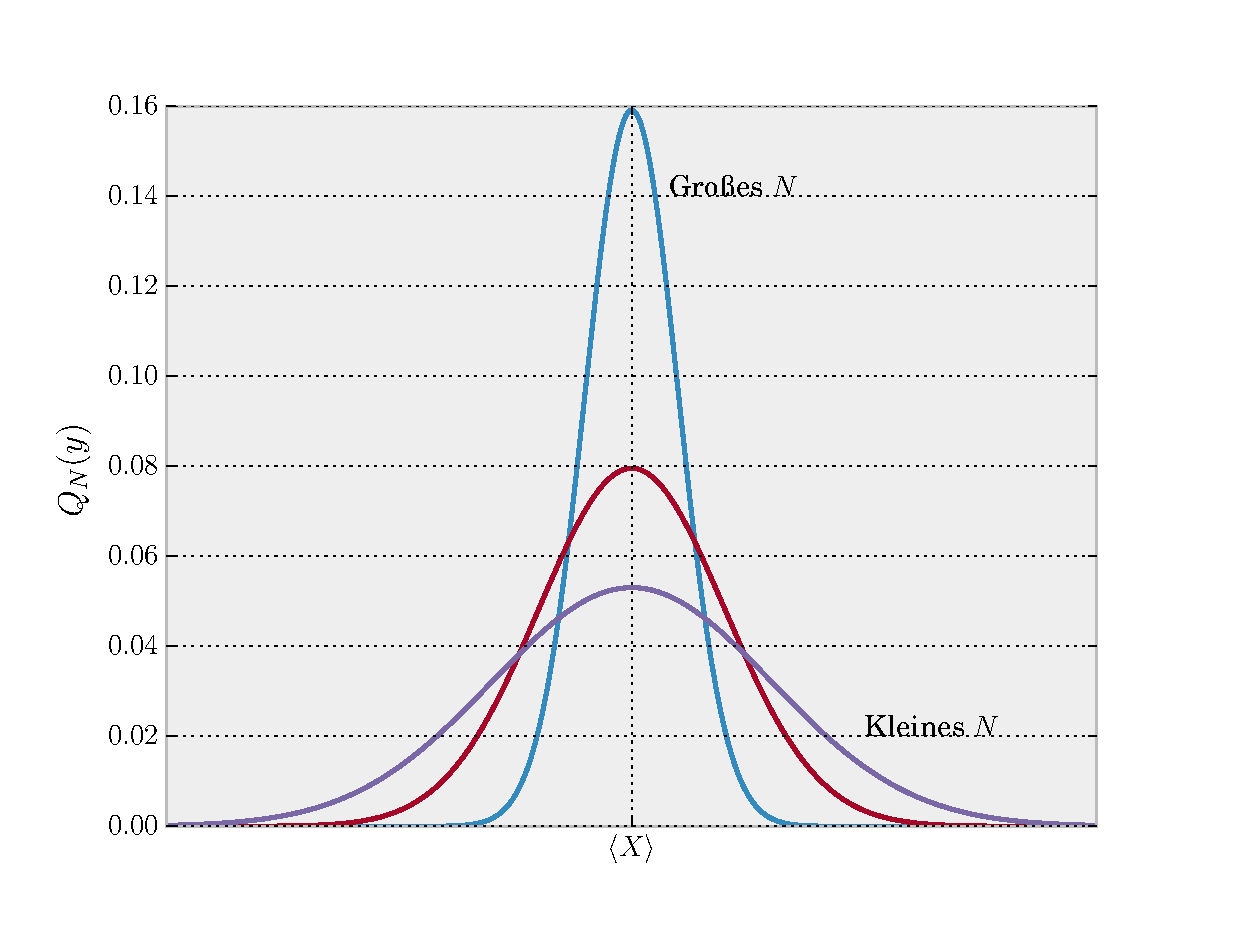
\includegraphics[width=0.8\textwidth]{./figures/first.eps}
  \caption{Normalverteilung, $Y=\Braket{X} \pm \frac{\Delta X}{\sqrt{N}} $}
  \label{fig:first}
\end{figure}
\section{Klassische Physik}
\begin{description}
  \item[N Teilchen ] Mikrozustand $(q,P) \in  \text{ Phasenraum } \simeq \R^{6n}$
  \item[Kanonische Gleichungen] \[ \dot{q}_j = \pd{H}{P_j} \quad \dot{P}_j = \pd{H}
    {\dot{q}_j}, \quad j=1,...,3N \] 
  \item[Anfangsbedingung] \[ (q_0, P_0)= (q_0(t_0), P(t_0)) \implies \text{ Bahn }
    (q(t | q_0, P_0), P(t| q_0, P_0)) \] 
  \item[Kanonische Transformation ] \[ (q(t), P(t)) \iff (q(t'), P(t')) \] 
  \item[Ziel] \[ \bar{A}= \int_{}^{} d^{3N}q\, d^{3N}p\, A(q,P) P_G(q,P) \] 
    Gleichgewichtsverteilung $P_G(q,P)= $?
  \item[Unscharfe Angangsbedingung] \[ P(q,P,t_0)= P_0 (q,P) \] 
    Scharfe Anfangsbedingung: $P_0(q,P) = \delta(q-q_0) \delta (P-P_0)$.
    Differentialgleichung f\"ur $P(q,P,t)$: Liouville-Gleichung.
    \[ P(t)= P(q,P,t)\, d^{3N}q\, d^{3N}p=P(t') = P(q,P,t')\, d^{3N}q'\, d^{3N}p' \] 
  \item[Liouville-Satz] \[ d^{3N}q\, d^{3N}p = d^{3N}q'\, d^{3N}p' \quad \left[
    \text{ Jacobi-Matrix } \frac{d^{3N}q'\, d^{3N}p'}{d^{3N}q\, d^{3N}p}= 1 \right] \] 
    \[ \implies P(q(t), P(t), t)= P(q(t'), P(t'), t'), \quad
    \text{ Erhalungsgr\"o\ss{}e } \frac{dP}{dt}=0 \] 
  \item[Kettenregel] \[ \frac{d P(q(t), P(t),t)}{dt}= \pd{P}{t} + \left\{ H,P \right\} \] 
  \item[Liouville-Gleichung] \[ \pd{P}{t}= \left\{ P,H \right\} \] 
    Bedingungen f\"ur $P_G(q,P)$ (im Gleichgewicht)
    \begin{itemize}
      \item $\left\{ P_G, H \right\}=0$
      \item $P_G \ge 0$
      \item $\int_{}^{}d^{3N}q\, d^{3N}p\, P_G (q,P)=1$.
    \end{itemize}
    Superpositionsprinzip: L\"osungen $P_1,P_2 \implies P=a_1 P_1+ a_2 P_2 $
    mit $a_1,a_2 \ge 0, \quad a_1+a_2 =1$. \\
    Makrozustand: $T,V,P,... \quad  \implies P_0 \text{ oder } P_g$?\\
\end{description}
\section{Quantenmechanik}

\emph{Schwabl Kapitel 1.4,1.5.2}\\
$N $ Teilchen, Mikrozustand $\Ket{\Psi} \in \mathcal{H} \simeq \mathcal{L}_2(\R^{3N})$
\begin{align*}
  i \hbar \frac{d}{dt} \Ket{\Psi(t)} = H \Ket{\Psi(t)} \\
  \text{Anfangsbedingung } \Ket{\Psi_0} \to \Ket{\Psi(t)} \quad \text{(eindeutig)} \\
  \text{Erwartungswert } A(t)= \Braket{\Psi(t) | \hat{A} | \Psi(t)} =\Braket{\hat{A}}\\
\end{align*}
Ziel: \[ \text{Statistische Mittelung } \quad \Braket{\hat{A}} = \trace(\hat{A}\hat{\rho}_G), \quad \hat{\rho}_G=? \] 
\subsubsection*{Definition}
Statistischer Operator, Dichteoperator, Dichtematrix, ...
\begin{align*}
  \hat{\rho} & : \mathcal{H} \to  \mathcal{H}, \text{ linear } \\
  \hat{\rho} & = \hat{\rho}^+\dagger \\
  \text{positiv-semidefinit } & \Braket{\varphi | \hat{\rho}| \varphi} \ge 0 \,\forall\,\Ket{\varphi} \in \mathcal{ H} \\
  \trace \hat{\rho } & =1  &
  \text{Spektrale Zerlegung } & \begin{split}
  \hat{\rho} &=  \sum_{n}^{} p_n \Ket{n}\Bra{n} \\ &= \int_{}^{} d \lambda \Ket{\lambda}\Bra{\lambda} w(\lambda) 
  \end{split}
   \\
  \text{Dichteoperator } & \implies \begin{matrix} p_n \ge 0 \\ \sum_{n}^{} p_n =1 \\
p_n \in \R \end{matrix} 
&
\begin{matrix} 
  w(\lambda )\ge 0 \\ \int_{}^{} d \lambda w( \lambda )=1 \\ w(\lambda) \in \R 
\end{matrix} \\
  \Braket{\hat{A}}= \sum_{n}^{}p_n \Braket{n|\hat{A}|n}.
\end{align*}
\begin{description}
  \item[Reiner Zustand]: \[ p_{n_0}=1,\, p_n =0 \,\forall\, n \neq n_0, \quad  \hat{\rho}= \Ket{n_0}\Bra{n_0} \implies \hat{\rho}^2=\hat{\rho} \]  
  \item[Gemisch]: $p_n \neq 0 $ f\"ur 2 oder mehr $n$.
    \begin{itemize}
      \item Verschr\"ankte Zust\"ande
      \item Statistisches Gemisch
    \end{itemize}
  \item[Spektrale Zerlegung] \begin{align*}
    \hat{A} &= \sum_{\alpha}^{}a_ \alpha \Ket{\alpha}\Bra{\alpha} \\
    \Braket{A}&= \sum_{n}^{}p_n \sum_{\alpha}^{}a_ \alpha \abs{\Braket{n|\alpha}}^2
    = \sum_{n}^{}\sum_{\alpha}^{} \underset{\text{Stat. Zufall}}{p_n} \underset{\text{Q.M. Zufall}}{\abs{\Braket{n|\alpha}}^2} a_ \alpha
  \end{align*}
  % TODO: Fig 4
  \[ \text{Gemisch: 2 Quellen: } I_1, \theta_1, \quad I_2, \theta_2 \implies 
  I'= I_1 ( \cos{\theta_1})^2 + I_2 (\cos{\theta_2})^2 \] 
  \[ p_1 = \frac{I_1}{I_1 + I_2}, \quad p_2 = \frac{I_2}{I_1 + I_2} \] 
\end{description}
\subsection*{Von Neumann Gleichung}
\[ i \hbar \frac{d\hat{\rho}}{dt} = \left[ H, \hat{\rho} \right] \] 
\begin{itemize}
  \item Anfangsbedingung $\hat{\rho}_0 \to  \hat{\rho}(t)$
  \item Gleichgewicht: \[ \frac{d \hat{\rho}}{dt}=0 \implies  \left[ H, \hat{\rho} \right]=0  \] 
  \item Superpositionsprinzip $\rho= a_1 \rho_1 + a_2 \rho_2 \text{ mit }
    a_1, a_2 \ge 0, \text{ und } a_1+a_2 =1 $
  \item Im Gleichgewicht: \[ \hat{\rho}_G = \sum_{n}^{} p_n \Ket{E_n}\Bra{E_n}
    = \int_{}^{} dE\, w(E)\Ket{E}\Bra{E} \quad \text{ mit }
    H \Ket{E}= E \Ket{E}\] 
  \item Isoliertes System: \[ p_n = \frac{1}{Z_n} \text{ f\"ur } E_n = E_0,
    \quad Z_n= \text{ Entartung des Niveaus } E_0 \] 
    % TODO: Fig 5
  \item Geschlossenes System: \[ p_n = \frac{1}{Z} e^{-\beta E_n} \text{ mit } 
    \beta= \frac{1}{k_B T}, \quad Z=\sum_{n}^{} e^{-\beta E_n} \] 
\end{itemize}

\subsection*{Entropie und Ensemble}
\emph{Schwabl Kapitel 2.1-2.5}\\
\begin{description}
  \item[Definition] Entropie (Quantenstatistik) \\
    \[ S =-k_B \trace(\hat{\rho} \ln{\hat{\rho}}) \quad k_B = k = 
      \text{ Boltzmann-Konstante }
    \approx \SI{1,38e-23}{\joule\per\kelvin} \] 
  \item[Eigenschaften] 
    \begin{align*}
      \hat{\rho} = \sum_{n}^{} p_n \Ket{n}\Bra{n} && p_n \ge 0 && \sum_{n}^{} p_n = 1 \\
      S(\left\{ p_n \right\}) = -k_B \sum_{n}^{} p_n \ln{p_n}
    \end{align*}
    Hinweise: \begin{align*}
      \trace \hat{A} = \sum_{n}^{} \Braket{n | \hat{A}|n} && f(\hat{\rho})= 
      \sum_{n}^{} f( p_n) \Ket{n}\Bra{n} \\
      e^{\hat{A}}= \sum_{n=0}^{ \oo } \frac{1}{n!}\hat{A}^n
    \end{align*}

    Die Entropie ist also \"uber die Diagonalemente der Dichtematrix in
    diagonalisierter Form berechenbar. Dies ist wohldefiniert, da jede
    Dichtematrix diagonalisiert werden kann.

    Extrema mit Nebenbedingung $\sum_{n}^{} p_n = 1$
    \begin{itemize}
      \item Minimum $S=0$ f\"ur einen reinen Zustand ($p_{n_0}=1, p_n =0
        \quad\forall\, n \neq n_0$)
      \item Maximum $S= k_B \ln{M}$ f\"ur $p_n = \frac{1}{M} \quad\forall\, 1,...,M$.
    \end{itemize}
    Die Entropie ist maximal f\"ur Unkenntnis \"uber den Zustand des Systems
    (Auch ma\ss{} f\"ur Unordnung).
  \item[Extensivit\"at] \[ \mathcal{H}= \mathcal{H}_A \otimes \mathcal{H}_B,
  \quad \hat{\rho} = \hat{\rho}_A \otimes  \hat{\rho}_B \] 
  \begin{align*}
    \hat{\rho}_A \to  \hat{\rho}_A \otimes  \hat{I}_B  \\
    \hat{\rho}_{\hat{B}} \to  \hat{I}_A \otimes  \hat{\rho}_B \\
    \implies \left[ \hat{\rho}_A, \hat{\rho}_B  \right]= 0
  \end{align*}
  \begin{align*}
    S & = -k_B \trace( \hat{\rho} \ln{\hat{\rho}})  \\
      & =  -k_B \trace \left[ (\hat{\rho}_A \otimes \hat{\rho_B}) 
  \ln{(\hat{\rho}_A \otimes \hat{\rho}_B)}  \right]  \\
  & = -k_B \trace (\hat{\rho}_A \ln{ \hat{\rho}_A}) - k_B \trace
    (\hat{\rho}_B \ln{ \hat{\rho}_B}) = S_A + S_B
  \end{align*}
  Nebenbedingung

  \[ S \le S_A + S_B \] (z.B. verschr\"ankte Systeme)
\item[Beispiel] System von $N$ Spins $S$ ($\vec{S}^2 =  S(S+1)$). \\
  Hilbert-Raum f\"ur einen Spin $= \mathcal{H}_1 = \C^{2S+1}$.
  Gesamter Hilbert-Raum \[ \mathcal{H} = \bigotimes_{i=1}^{N} \mathcal{H}_i \] 
  \[ \operatorname{dim} \mathcal{H} = (2S+1)^N = M \] 
  \begin{itemize}
    \item Minimum $S=0$ z.B. f\"ur $\Ket{\Psi} = \Ket{ \uparrow, \uparrow, \uparrow, \ldots, \uparrow}$.
    \item Maximum $S= k_B \ln{M}$ f\"ur $\hat{\rho}= \frac{1}{n} \hat{I}=
      k_B n \ln{(2S+1)}$
  \end{itemize}
\item[Gleichgewicht]
  \begin{align*}
    0= \frac{d \rho }{dt} \iff \left[ H, \hat{\rho} \right]=0 \implies 
    \rho = \sum_{m}^{} p_n \Ket{E_n} \Bra{E_n} \\
    \implies E = \Braket{\hat{H}} = \trace (\hat{\rho} \hat{H})
    = \sum_{n}^{} p_n E_n
  \end{align*}
  \begin{align*}
    \rho \Ket{E_n} = p_n \Ket{E_n} \\
    H \Ket{E_n} = E_n \Ket{E_n}
  \end{align*}
\end{description}
\begin{description}
  \item[Definition]  Statistisches Ensemble oder Gesamtheit \\
    Sie ist eine Gewichtete Menge der Mikrozust\"ande, die einen 
    Makrozustand entsprechen.
    \begin{align*}
      \left\{ ( \Ket{N}, p_n) \right\} \equiv \hat{\rho} = \sum_{n}^{} p_n
      \Ket{n} \Bra{n} 
    \end{align*}
\end{description}
\subsection*{Zentrales Postulat der statistischen Physik}
System mit $N\to \infty$ Freiheitsgraden im Gleichgewicht.
\begin{itemize}
  \item $S$ ist maximal f\"ur einen gegebenen Makrozustand. Das erlaubt uns
    eine eindeutige bestimmung des statistischen Operators $\hat{\rho}$.
  \item Statistische Mittelungen der Observablen erf\"ullen die Makroskopischen
    Gesetze der Thermodynamik.
    %
    \begin{align*}
      S = -k_B \trace \hat{\rho}_B = - k_B \Braket{\ln{\hat{\rho}_G}} \\
    \end{align*}
    %    
    \begin{align*}
      \Braket{\hat{\cal{O}}}= \trace (\hat{\rho}_G \mathcal{O}) &&
      U = \Braket{\hat{H}}
    \end{align*}

\end{itemize}
\begin{description}
  \item[Definition] Entropie (Thermodynamik) \\
    Wir betrachten ein System in einem Bad, mit welchem es Energie austauschen
    kann. Eine ideelle Situation, in welcher alle Prozesse die wir betrachten 
    reversibel sind. 
    \begin{align*}
      dS = \frac{\delta Q}{T}
    \end{align*}
    Zustandsfunktion oder Thermodynaische Variable.
    \begin{itemize}
      \item Extensiv
      \item monoton steigend $\pd{S}{E} > 0$
      \item $ \lim_{T \to 0} \frac{S}{N} = 0$.
    \end{itemize}
\end{description}
\begin{description}
  \item[Nebenbedingung] F\"ur bestimmte Modelle statistische Entropie nicht
    gleich der thermodynamischen Entropie, das bedeutet das Modell ist nicht
    physikalisch. Eigentlich hat man in den letzten 100 Jahren in denen man
    Forschung betreibt kein Problem gefunden, das man nicht l\"osen konnte.
    Es gibt verschiedene Situationen in derr Praxis, in denen man die Makrozust\"ande
    beschreibt. 
\end{description}
\subsection*{Mikrokanonisches Ensemble}
Es beschreibt ein isoliertes System.
\begin{description}
  \item[Freie thermodynamische Variablen] $ $ 
    \begin{itemize}
      \item Teilchenzahl $N$
      \item Volumen $V$
      \item Magnetisierung $M$
      \item Energie $E$
    \end{itemize}
  \item[Zustandsfunktion] Druck $P(N,V,E)$
  \item[Maximierung der Entropie] 
    \begin{align*}
      \hat{\rho} & = \subset P_E P_N \ldots \\
      \hat{\rho} & ~ \delta(\hat{H} - E) \delta (\hat{N} - N)
    \end{align*}
\end{description}
\subsection*{Kanonisches Ensemble}
Beschreibt ein geschlossenes System.
\begin{description}
  \item[Freie thermodynamische Variablen] $ $
    \begin{itemize}
      \item Temperatur $T$
      \item $N, V, M$
    \end{itemize}
  \item[Zustandsfunktionen] $E(T, N, V)$
  \item [Maximum der Entropie] 
    F\"ur feste $T, N, V, \ldots$
    \begin{align*}
      \hat{\rho} = \frac{1}{Z} e^{- \beta \hat{H} } \hat{P}_N \ldots && 
      \beta = \frac{1}{k_B T}
    \end{align*}
  \item[Zustandsumme]
    \begin{align*}
      Z= \trace e^{- \beta \hat{H}}
    \end{align*}
\end{description}

\subsection*{Gro\ss{}kanonisches Ensemble}
Beschreibt ein offenes System
\begin{description}
  \item[Freie Thermodynamische Variablen]  $ $
    \begin{itemize}
      \item Chemisches Potential $\mu$
      \item $T, V, \ldots$
    \end{itemize}
  \item[Zustandsfunktionen] $N(T, \mu, V)$
  \item[Maximum der Entropie] f\"ur feste $T, \mu, V$ falls
    \begin{align*}
      \hat{\rho}_G = \frac{1}{Z_{GK}} e^{-\beta(\hat{H}- \mu \hat{N})} P
    \end{align*}
  \item[Gro\ss{}kanonische Zustandssumme] $Z_{GK} 
    \trace e^{-\beta(\hat{H}- \mu \hat{N})} $
\end{description}
\subsection*{Viele weitere Ensembles}
Zu jeder intensiven Variable gibt es eine Extensive Variable(Observable).

\begin{center}
  \begin{tikzpicture}
    \matrix (m) [matrix of math nodes,column sep=6em,
      column 1/.style={anchor=base east},
      column 2/.style={anchor=base west}
    ] 
    {
      \underset{\text{Intensive Variable}}{\text{\"Au\ss{}eres Feld}} & 
      \underset{\text{Extensive Variable}}{\text{Observable}} \\
      y & x \\
      \hat{\rho}_G ~ e^{- \beta y \hat{x}} & \hat{\rho}_G ~ 
      P_x ~ \delta (\hat{x} -x ) \\
      \text{Beispiele} \\
      M & N \\
      P & V \\
      H & M \\
    \text{Magnetfeld} & \text{Magnetisierung} \\};
  \end{tikzpicture}
\end{center}


 \section*{Mikrokanonisches Ensemble}
 Wir betrachten ein isoliertes System. Zum beispiel ein Gas in einem Beh\"alter
 welcher isoliert ist. Energie und Teilchenzahl sind fest. Genauso das Volumen.
 Eine \"Ahnliche Situation w\"are auch ein magnetisches Material. Die isolation
 w\"are hier ein Material welches keine magnetischen Felder durchl\"asst.
 Typisch f\"ur das isolierte System ist, dass die Energie eine kontrollierbare
 Variable ist.

 Es gibt also eine Freie thermodynamische Variable $E$. Die erlaubten 
 Mikrozust\"ande sind die Eigenzust\"ande des Hamilton-Operators $H$ zur
 Energie $E$.
 Das Ziel ist nun die mikrozust\"ande zu beschreiben und die makroskopischen
 Variablen zu berechnen. Man braucht dazu den statistischen Operator.
 \begin{description}
   \item[Diskretes Eigenspektrum] 
     \begin{align*}
       \hat{\rho} = \sum_{n}^{} p_n \Ket{n}\Bra{n} \quad : \quad \mathcal{H} \to 
       \mathcal{H} && p_n =0 \quad\forall\, n \text{ mit } E_n \neq E \\
       \hat{\rho}= \sum_{n=1}^{w(E)} p_n \Ket{n}\Bra{n} &&
       w(E) = \text{ Entartung der Eigenergie } E
     \end{align*}
     Wir verwenden das Postulat der maximierung der Entropie:
     \begin{align*}
       S(E)= -k_B \sum_{n=1}^{w(E)} p_n \ln{p_n}, && 
       \sum_{n=1}^{w(E)} p_n = 1 
     \end{align*}
     \begin{align*}
       0  &= \pd{S}{p_n} - \lambda \pd{}{p_n} 
       \left( \sum_{n=1}^{w(E)} p_m -1 \right)  \\
       & = -k_B \left( \ln{p_n} +1 \right) - \lambda \Forall 1 ,\dotsc, w(E) \\
     \end{align*}

     \begin{align*}
       \text{ Extrema f\"ur }      
       & \implies p_n = e^{-\frac{\lambda}{k_B} - 1} \implies p_n = \frac{1}{w(E)} \\
       & \implies S(E) = k_B \ln{(w(E))} \text{ ist auch ein Maximum }
     \end{align*}

   \item[Dichteoperator im Gleichgewicht]
     \begin{align*}
       \hat{\rho}_G = \sum_{n=1}^{w(E)} \frac{1}{w(E)} \Ket{n}\Bra{n} =
       \frac{1}{w(E)} P_E = \frac{1}{w(E)} \delta(H-E) & \\
     \end{align*}
     \begin{align*}
       \trace \hat{\rho}_G = 1 && \trace P_E = w(E) \\
     \end{align*}

   \item[Kontinuierliches Spektrum]
     \begin{flalign*}
       \hat{\rho} &= \int_{}^{} d\lambda\, \Ket{\lambda}\Bra{\lambda} p(\lambda) \\
       N(E) &= \text{ Anzahl der Zust\"ande mit einer Eigenenergie } \le E
     \end{flalign*}
     Hinweis: F\"ur ein diskretes System von Eigenzust\"anden
     f\"ur ein kontinuerliches Spektrum kann man die Anzahl der Eigenzust\"ande 
     kleiner Als $w$ definieren.
     \begin{align*}
       w(E) &= \frac{dN}{dE} = \text{ Zustandsdichte } \\ & \implies w(E) \Delta E
       = \text{ Anzahl der Eigenzust\"ande in } \left[ E, E+ \Delta E \right] \\
       S(E) &= k_B \ln{(w(E) \Delta E)} \\
       \hat{\rho} &= \frac{1}{w(E)} \delta(H-E) 
     \end{align*}
 \end{description}
 \subsection*{Thermodynamische Variablen}
 Man macht eine Statistische Mittelung
 \begin{align*}
   \Braket{\hat{\cal{O}}} = \trace (\hat{\rho}_G \hat{\cal{O}})
 \end{align*}
 \begin{description}
   \item[Beispiele] 
     \begin{align*}
      \text{Innere Energie: } U= \Braket{H} = E \\
      \text{Magnetisierung: } M_z = \Braket{S_z} \\
     \end{align*}
   \item[Thermodynamischer Limes] ($N \to \infty$)
   \item[Definition] Temperatur
     \begin{align*}
       \frac{1}{T} = \left( \pd{S}{E} \right)_x
     \end{align*}
   \item[Definition] Konjugierte Variablen \\
     Beispiele: 
     \begin{align*}
       x = \begin{Bmatrix} 
         M \xleftrightarrow{\hspace{1cm}}  H \\ 
         N \xleftrightarrow{\hspace{1cm}}  M \\
         V \xleftrightarrow{\hspace{1cm}} P 
     \end{Bmatrix} y
     \end{align*}
     %
     \begin{align*}
       S(E,X) && y = \pm  T \left( \pd{S}{X} \right)_E
     \end{align*}
     %
   \item[Statistische Physik] $ $ \\
     \begin{align*}
       \text{Extensive Observable } \hat{x}, \quad && [\hat{x}, \hat{H}]
       \xrightarrow{ N \gg 1} N^0, n^{-1} \\
       \implies \Braket{\hat{x}} = x && S(E,X) = k_B \ln{ w(E,X)} \\
     \end{align*}
 \end{description}
\subsection*{Beispiel: System von nicht-wechselwirkenden Spins}
\begin{align*}
  N \text{ Spins } s=1, && H = \sum_{i=1}^{ N } H_i = J \sum_{i=1}^{N} S_{iz}^z
  \quad (J>0) \\
\end{align*}

Eigenzust\"ande: 

\begin{align*}
  \text{1 Teilchen } & \begin{cases}
    H_i \Ket{M_j} = J S_{j z}^z \Ket{m_j} = J \hbar^2 m_j^2 \\
    S_{zj} \Ket{m_j} = \hbar m_j \Ket{m_j} &  m _j = -1,0,1 \\
  \end{cases} \\
  \text{$N$ Teilchen } & \begin{cases}
    \text{Dim } \mathcal{H} = 3^N \\ %REALLY? \\
    \Ket{ \left\{ m_j \right\} }= \Ket{m_j} \otimes \Ket{m_j} \otimes  \ldots 
      \otimes  \Ket{m_N} \\
      E(\left\{ M_j \right\})= J \sum_{j=1}^{N}m_j^2 \\
      S_z \Ket{ \left\{ m_j \right\} }= {\sum_{j}^{} m_j } & M=\sum_{j}^{}
      m_j
      \Ket{ \left\{ m_j \right\} }
  \end{cases} \\
  & H\Ket{ \left\{ m_j \right\} } = E (\left\{ m_j \right\}) \Ket{ \left\{ m_j \right\} }
\end{align*}

\begin{description}
  \item[Problem]  Entartung $w(E,M)$ \\
    \begin{align*}
      N_+ & = \text{ Anzahl der Spins mit } m_j = +1 \text{ in } \left\{ m_j \right\}\\
      N_0 & = \text{ Anzahl der Spins mit } m_j = +0 \text{ in } \left\{ m_j \right\}\\
      N_- & = \text{ Anzahl der Spins mit } m_j = -1 \text{ in } \left\{ m_j \right\}\\
    \end{align*}

    \begin{align*}
      \implies \begin{cases}
        E = J (N_+ + N_-) \\
        M = N_+ - N_- \\
        N = N_+ +N_- + N_0 \\
      \end{cases}
      \implies \begin{cases}
        N_+ = \frac{R+M}{L} =  \frac{r+m}{ L}N \\
        N_- = \frac{R-M}{L} = \frac{r - m}{ L} N\\
        N_0 = N-R = (1- r ) N \\
      \end{cases}
    \end{align*}

    \begin{align*}
      \text{Energie pro Spin ist } r= \frac{R}{N}= \frac{E}{NJ} \quad \in [0, 1] \\
      \text{Magnetisierung pro Spin } m = \frac{M}{N} \quad \in [-1, 1]
    \end{align*}

    Problem: $N_+$ unterscheidbare Zust\"ande $m_j= +1$ auf $N$ Spins verteilen.

    \begin{align*}
    & \implies \begin{pmatrix} N \\ N_+ \end{pmatrix} = \frac{N!}{N_+!(N-N_+)!}
      \text{ M\"oglichkeiten }  \\
      \end{align*}

      Danach: $N_-$ unterscheidbare Zust\"ande auf $N-N_+$ Spins mit
      $m_j = -1$ verteilen.
      \begin{align*}
      \implies \begin{pmatrix} N-N_+ \\ N_- \end{pmatrix} \text{ Moeglichkeiten} 
      \end{align*}

      Also insgesamt:
      \begin{align*}
       w(E,M) & = w(N_+, N_-) \\
      & = 
      \begin{pmatrix} N \\ N_+ 
      \end{pmatrix}  
      \begin{pmatrix} N-N_+ \\ N_- 
      \end{pmatrix} \\ & = \frac{N!}{N_+! N_-! N_0!} 
      \end{align*}

      Damit folgt die Entropie:
      \begin{align*}
        \begin{split}
         S(E,M) & = S(N_+, N_-) \\ &= k_B \ln{}\left( 
        \frac{N!}{N_+! N_-! N_0! }\right) 
      \end{split}
    \end{align*}
  Annahme: $N, N_+, N_0, N_- \gg 1$ aber
    
    \begin{align*}
      & \frac{N_+}{N}, \frac{N_-}{N}, \frac{N_0}{N} \text{ fest und endlich } \\
      \iff & m,n \text{ fest und endlich} \\
      \iff & M,E \text{ sind extensiv } (M,E \propto N)
    \end{align*}
    Stirling Formel \begin{align*}
      & \ln{N!} \approx N \ln{N} - N \\
      \implies & S(E, M) = k_B N f(r, m) \\
      f(r, m ) & = - \left[ \frac{r+m}{2} \ln{(r+m)} + \frac{r - m}{2}
    \ln{\frac{(r - m)}{2}} + (1-r) \ln{(1 - r)} \right]
    \end{align*}
  \item[Temperatur]
    \begin{align*}
      \frac{1}{T} = \left( \pd{S}{E}  \right)_M = \frac{k_B}{J} 
      \ln{\left( \frac{2 (1-r)}{ \sqrt{r^2 - m^2}} \right)}
    \end{align*}
  \item[Ohne Magnetisierung] $M=0$ genau dann, wenn $m=0$.
    \begin{align*}
      S(E) = - k N [ r \ln{\frac{r}{2}} + (1-r) \ln{(1-r)}] \\
    \end{align*}
    %
    \begin{align*}
      \frac{1}{T} = \frac{k_B}{ J } \ln{\left( \frac{2 ( 1-r)}{r} \right) }
       \begin{cases}
         > 0 & \text{ falls } 0 < r < \frac{2}{3} \\
         < 0 & \text{ falls }\frac{2}{3} < r < 1 \\
      \end{cases}
    \end{align*}
    \begin{align*}
      \implies  r (T) &= \frac{2}{e^{\beta J }+2 }, \quad  \beta= \frac{1}{k_B T} \\
                E(T)  &= NJ \frac{2}{e^{\beta J}} \frac{2}{e^{\beta J} + 2} \\
                S(T)  &= k N \left[ \frac{2}{e^{\beta J} + 2} \ln{(e^{\beta J} + 2)}
    - \frac{1}{e^{-\beta J} + 2} \ln{ \left( 1+ 2 e^{-\beta J} \right) }\right]
    \end{align*}
  \item[Diskussion] $ $  \\
    Tiefe Temperaturen \begin{align*}
      k_B T \ll J \iff \beta J \longrightarrow \infty \quad \implies \begin{cases}
        E \longrightarrow 0 \\ S \longrightarrow 0
      \end{cases}
    \end{align*}
    Nebenbedingung f\"ur $J < 0$: 
    \begin{align*}
      \implies  \begin{cases}
        E = N J \\
        S = k_B N \ln{(z)}
      \end{cases}
    \end{align*}

    Hohe Temperatur $k_B T \gg J$

    \begin{align*}
      \iff \beta J \longrightarrow  0 \implies 
      \begin{cases}
        E = \frac{2}{3} N J \\
        S = \frac{1}{3} k_B N \ln{(3)}
      \end{cases}
    \end{align*}
\end{description}
\subsection*{Kanonisches Ensemble}
\emph{Schwabl Kapitel 2.6} \\
Schwabl nimmt an, dass man das gesamte System mikrokanonisch behandeln kann.
$\hat{\rho} \propto \delta (\hat{H} -E)$. Das innere Teilsystem 2 ist
viel kleiner als das \"au\ss{}ere Teilsystem 1. Also ist auch die \"anderung
der Energie des Systems 1 $\Delta E_1 \gg \Delta E_2$. Man benutzt dann
das Prinzip der maximierung der Entropie $S$ woraus folgt, dass
%
\begin{align*}
  \hat{\rho}_2 = e^{- \hat{H}_2 / (k_B T_2) }
\end{align*}
%
Quantenmechanik Anmerkung:
%
\begin{align*}
  \mathcal{H} = \mathcal{H}_1 \otimes \mathcal{ H}_2 && \text{ Basis } 
  \left\{ \Ket{n_1} \otimes \Ket{n_2} \right\} \text{ von } H
\end{align*}
%
\begin{align*}
  \trace \hat{A} = \sum_{n}^{} \Braket{n | \hat{ A} | n} = 
  \sum_{n_1}^{} \sum_{n_2}^{} \Braket{n_1 n_2 | \hat{A} | n_1 n_2} 
\end{align*}
%
%
\begin{align*}
  \hat{A}_1 & = \trace_{\mathcal{H}_1} \hat{A} = \sum_{n_2}^{} \Braket{n_2 | \hat{A} | n_2} \\
            & = \sum_{n_2}^{} \sum_{n_1}^{} \sum_{n_1'}^{} 
  \Braket{ n_1 n_2 | \hat{A} | n_1' n_2} \Ket{n_1} \Bra{n_1'}
\end{align*}
%

%

%
\begin{align*}
  \hat{\rho}_1 = \trace_{\mathcal{H}_1} \hat{\rho} \implies S_1 (E_1) = 
  \frac{1}{T_1} = \left( \pd{S_1}{E_1} \right) = \frac{1}{T} .
\end{align*}
%

Wir betrachten ein geschlossenes System im Gleichgewicht mit W\"armebad der 
Temperatur $T$. Was ist der statistische Operator $\hat{\rho}$ ?

\begin{description}
  \item[Definition]  Freie Energie (Thermodynamik, makroskopisch)
    %
    \begin{align*}
      F(T) = U(S(T)) - T S(T)
    \end{align*}
    Legendre-Transformation
    %
    \begin{align*}
      \frac{1}{T} = \left( \pd{S}{E} \right)_X \iff T_X =
      \left( \pd{E}{S} \right)_X \\
      \implies S = - \left( \pd{F}{T} \right)_X
    \end{align*}
    %
  \item[Postulat] Im thermischen Gleichgewicht ist die Entropie maximal. 
    Dies gilt genau dann wenn die freie Energie minimal ist.
    %
  \item[Definition] Funktional der freien Energie In der 
    mikroskopischen statistischen Physik.
    % 0
    \begin{align*}
      F[\hat{\rho}] & = E[\hat{\rho}] - T S [\hat{\rho}] \\
                    & \text{mit } E [\hat{\rho}] = \Braket{\hat{ \mathcal{H}}}
      = \trace (\hat{\rho} \hat{ \mathcal{H}})
    \end{align*}
    %
  \item[Minimierung von ] $F[\hat{\rho}]$ \\
    Variationsrechnung $\delta F= 0 \quad\forall\, \delta \hat{\rho}$
    \begin{enumerate}
      \item %
      \begin{align*}
          \delta F & = F \left( \hat{\rho} + \delta \hat{ \rho} \right) -
          F \left( \hat{\rho} \right) \\ & = \trace (H \delta \hat{\rho}) 
        + k_B T \trace (\delta \hat{\rho} \ln{\hat{\rho}}) + k_B T \trace
        \delta \hat{\rho} \\ & = \trace ( ( H+ k_B T \ln{ \hat{\rho}}) \delta \hat{\rho}) \\
      \end{align*}
      Wir verwenden, dass man kompakte operatoren in der Spur vertauschen kann.
      %
      \begin{align*}
        \trace (\hat{A} \hat{B}) = \trace (\hat{B} \hat{A})  \\
        \trace \hat{\rho} = 1 \implies \trace \delta \hat{\rho} = 0
      \end{align*}
      %
    \item
      %
      \begin{align*}
        \delta F = 0 \quad\forall\, \delta \hat{\rho} \implies 
        H + k_B \ln{\hat{\rho}} = c \iff
        \hat{\rho} = e^{ \frac{\hat{H}}{k_B T} } e^{ \frac{c}{ k_B T}} \\
      \end{align*}
      %
      Die folgenden drei Formeln sollte man sich merken:
      \begin{align*}
        \implies \hat{\rho} = \frac{1}{Z} e^{-\beta \hat{H}} && \beta = \frac{1}{k_B T} \\
      \end{align*}
      %
      \emph{Kanonische Zustandsumme}
      \begin{align*}
         Z = \trace e^{-\beta \hat{H}} 
      \end{align*}
      %
      Minimum von $F[\hat{\rho}] \equiv $ Freie Energie.
      %
      \begin{align*}
        F = -k_B T \ln{Z} 
      \end{align*}
      %
      Bemerkung: $\hat{\rho} = e^{-\beta \hat{H}} P_N$ %TODO
    \end{enumerate}
    Weitere thermodynamische Variablen %
    \begin{align*}
      x = \trace (\hat{\rho} \hat{x}) \text{ z.B. } M,N
    \end{align*}
    %
    %
    \begin{align*}
      \text{Thermodynamik } y = \pm \left( \pd{F}{X}  \right)_T, 
      \text{ z.B } P = - \left( \pd{F}{V} \right)_T, B = 
      \left( \pd{F}{M} \right)_T
    \end{align*}
    %
\end{description}
\subsection*{Statistische Bedeutung der W\"arme}
%
\begin{align*}
  dE & = d \trace \left( \hat{\rho} \hat{H} \right) = 
  \trace\left( d \hat{\rho} \hat{H} \right) + 
  \trace \left( \hat{\rho} d \hat{H} \right)  \\
  dS & = -k_B d \trace \left( \hat{\rho} \ln{ \hat{\rho}} \right) = 
  - k_B \trace \left( d \hat{\rho} \ln{ \hat{\rho}} \right) - k_B \trace d \hat{\rho} \\
   & \underset{\hat{\rho} = \frac{1}{z } e^{- \beta \hat{ H}}}{=} 
  \frac{1}{T} \trace (d\rho \hat{H}) \\
\implies & dE = T dS + \trace \left( \hat{\rho} d \hat{H} \right).
\end{align*}
\emph{1. Hauptsatz der Thermodynamik} 
%
\begin{align*}
  dV = \delta Q + \delta A
\end{align*}
%
\begin{itemize}
  \item Reversibler Prozess
    %
    \begin{align*}
      \delta Q & = T dS = \trace \left( d \hat{\rho} \hat{H} \right) \\
      \delta A & = \trace \left( \hat{\rho} d \hat{H} \right)
      \implies & \text{ \"Anderung der W\"arme $\equiv$ 
    \"Anderung der Wahrscheinlichkeit der Mikrozust\"ande}
    \end{align*}
    %
\end{itemize}
\subsection*{Energiefluktuationen}
Wahrscheinlichkeit f\"ur Mikrozustand mit Energie $E$.
Diskretes Spektrum 
%
\begin{align*}
  P(E) = 
  \begin{cases}
    \frac{1}{Z} e ^{-\beta E} & \text{ Falls Eigenenergie $E$ existiert} \\
    0                         & \text{ Falls Eigenenergie $E$ nicht existiert} \\
  \end{cases}
  \end{align*}
%
Kontinuerliches Spektrum 
%
\begin{align*}
  P(E) & = W(E) \Delta E \\
  W(E) & = w(E) \frac{1}{Z} e^{-\beta E} \\
\end{align*}
%
Definition einiger Gr\"o\ss{}en
\begin{itemize}
  \item Mittelwert 
    %
    \begin{align*}
      \bar{E} = \int_{}^{} \d{E} w(E) E = \Braket{\hat{H}} = U
    \end{align*}
    Nebenbedingung
    %
    \begin{align*}
      \Braket{H} = -\pd{}{\beta} \ln{Z} 
    \end{align*}
  \item Schwankungsquadrat 
    %
    \begin{align*}
      \Delta E ^2 = \int_{}^{} \d{E} W(E) \left( E- \bar{E} \right) ^2 
      = \Braket{\hat{H}^2} - \Braket{\hat{H}} ^2
    \end{align*}
    %
    Nebenbedingung
    %
    \begin{align*}
      \Delta E^2 = - \pd{\bar{E}}{\beta} = - \pd{\Braket{\hat{H}}}{\beta}
    \end{align*}
    %
  \item W\"armekapazit\"at 
    %
    \begin{align*}
      C_x = \left( \frac{dU}{dT} \right)_x = \frac{1}{k_B T^2} \Delta E^2 &&
      \beta = \frac{1}{k_B T}
    \end{align*}
    %
    3. Hauptsatz
    %
    \begin{align*}
      \lim_{T \to  0} C_x = 0 \implies \lim_{T\to  0 } \Delta E^2 = 0 
    \end{align*}
    %
\end{itemize}
\subsection*{Relation mit dem mikrokanonischen Ensemble}
Experiment: $U$ und $C_x$ sind extensiv. Das bedeutete mathematisch, dass
$U$ und $C_x$ proportional zur Teilchenzahl $N$ sind. Das bedeutet auch, dass
der Mittelwert $\bar{E}$ und das Schwankungsquadrat $\Delta E$ proportional 
zur Teilchenzahl sind. Das bedeutet f\"ur die relative Breite:
%
\begin{align*}
  \frac{\Delta E}{\bar{E}} \propto \frac{1}{\sqrt{N}} 
  \xrightarrow{\text{Thermodynamischer Limes}} 0
\end{align*}
%
% zeichnung
%
%
\begin{align*}
  P(\bar{E}) & = W(\bar{E}) \Delta E \xrightarrow{n\to\infty} 1 \\
  \text{ oder } & W(E) \to \delta(E - \bar{E})
\end{align*}
%
\"Aquivalenz der mikrokanonischen und kanonischen Ensembles im
thrmodynamischen Limes $( \frac{\Delta E}{N} \to 0)$.

\subsection*{Beispiel: Spin System}
%
\begin{align*}
  \hat{H} = J \sum_{i=1}^{N} S_{iz}^z - B \sum_{i=1}^{N} S_{iz} 
  = \sum_{i=1}^{N} H_i
\end{align*}
%
%
\begin{align*}
  \hat{\rho} = \frac{1}{z} e^{-\beta \hat{H}}  &&
  \left[ H_j, H_l \right] = 0 \quad\forall\, j,l = 1,\dotsc,N
\end{align*}
%
%
\begin{align*}
  Z = \trace_\mathcal{H} e^{-\beta \hat{H}} = \trace_{\mathcal{H}_1} e ^{-\beta \hat{H}_1} \trace
  e^{-\beta \hat{H}_2} \ldots \trace_{\mathcal{H}_N} e^{-\beta \hat{H}_N}
\end{align*}
%
%
\begin{align*}
  Z_1 = \trace_{\mathcal{H}_1} e^{-\beta \hat{H}_1} = \sum_{m_1=1,0,1}^{}
  \Braket{m_1 | e^{-\beta \hat{H}_1} | m_1} \\ \hat{H}_1 \Ket{m_1} = 
  \left( J m_1^2 - \beta m_1 \right) \Ket{m_1}
\end{align*}
%
%
\begin{align*}
  \implies & Z_1 = 1 + e^{-\beta (J+B)} + e^{-\beta (J-B)} \\
  \implies & Z = \left( 1 + e^{-\beta (J+B)} + e^{-\beta(J-B)} \right)^N
  & = \left( 1+2 e^{-\beta J} \cosh(\beta B) \right)^N
\end{align*}
%
%
\begin{align*}
  Z = \left( 1 + Z e ^{-\beta J} \cosh(\beta B) \right)^N 
\end{align*}
\emph{Freie Energie}
%
\begin{align*}
  F(T, X) = - k_B T \ln{Z (T, X)} && X = V, M \\
\end{align*}
\emph{Freie Enthalpie} 
%
\begin{align*}
  G (T, Y) = -k_B T \ln{Z(T, X)} && y = P, B
\end{align*}
\emph{Legendre Transformation}
%
\begin{align*}
  G(T, B) = F (T, M(T, B)) - M(T,B) B
\end{align*}
%
\begin{align*}
  B = \left( \pd{F}{M} \right)_T && M = - \left( \pd{G}{B} \right)_T
\end{align*}
%
%
\begin{align*}
  \implies G(T,B) = -k_B T N \ln{\left( 1+ 2 e^{- \beta J} \cosh{\beta B} \right)}
\end{align*}
%

\begin{description}
  \item[Magnetisierung] 
    %
    \begin{align*}
      M & = \Braket{S_z} = \frac{1}{Z} \trace (e^{-\beta \hat{H}} \hat{S}_z) \\
        & = \frac{1}{\beta} \pd{\ln{ Z}}{\beta} \\
        & = N \frac{2 e^{-\beta J} \sinh(\beta B)}{1 + 2 e^{-\beta J} \cosh
    (\beta B)}
    \end{align*}
    anmerkung:
    %
    \begin{align*}
      Z = \trace e^{-\beta H} && H = J \sum_{i}^{} \hat{S}_{iz}^z - B \sum_{i}^{}
      S_{iz}
    \end{align*}
    %
    \begin{itemize}
      \item Tiefe Temperatur $k T \ll J, \abs{B}$
        \begin{itemize}
          \item Falls $\abs{B} < J$ so geht $M \to 0$ \\
          \item Falls $\abs{B} < J$ so geht $M \to \tanh(\beta B) \to N \sign(B)$
            Im Grundzustand $ \Ket{m_1 = \sign B}$.
        \end{itemize}
    \item Hohe Temperatur $k T \gg J, \abs{B}$ \\
        %
        \begin{theorem*}[ Curie-Gesetz ]
            \begin{align*}
                M = N \frac{2}{3} \frac{B}{k_B T}
            \end{align*}
        \end{theorem*}

        %
        
    \end{itemize}
\end{description}
\subsection*{Gro\ss{}kanonisches Ensemble}
\emph{Schwabl Kapitel 2.7} \\
Wir haben einen offenen Beh\"alter, in dem sich ein Untersystem befindet.
Man kontrolliert nicht die Teilchenzahl und die Energie, sondern nur die TEmperatur
und das chemische Potential.
Es handelt sich also um ein offenses System im Gleichgewicht mit
\begin{itemize}
  \item Einem W\"armebad bei Temperatur $T$.
  \item Einem Teilchenreservoir mit chemischem Potential $\mu$.
\end{itemize}
\begin{beispiel} Wasserspiegel
    
\end{beispiel}

% insert graphics here
\begin{definition} Gro\ss{}kanonisches Potential der Thermodynamik
    %
    \begin{align*}
      \Phi(T, \mu) = U\left( S (T, \mu), N(T, \mu) \right) - 
      T S(T, \mu)  - \mu N(T, \mu) 
    \end{align*}
    %
    %
    \begin{align*}
      T = \left( \pd{U}{S} \right)_{X, N} && \mu = \left( \pd{ U}{N} \right)_{X, T} \\
      S = - \left( \pd{F}{T} \right)_{X, \mu} && N = -\left( \pd{\Phi}{\mu} \right)_{X, T} \\
    \end{align*}
\end{definition}

%
\begin{postulat}
    Thermodynamisches Gleichgewicht besteht genau dann, wenn
    die Entropie $S$ maximal ist. Oder \"Aquivalent, das gro\ss{}kanonische
    Potential $\Phi$ minimal ist.
\end{postulat}

\begin{definition}
    Funktional des gro\ss{}kanonischen Potentials
    (Statistische Physik)
    %
    \begin{align*}
        \Phi[\hat{\rho}] = E \left[ \hat{\rho} \right] - T S [\hat{\rho}]
        - \mu N[ \hat{\rho}]
    \end{align*}
    %
    wobei %
    \begin{align*}
        N [\hat{\rho}] = \trace (\hat{\rho} \hat{N})
    \end{align*}
    %
\end{definition}
        
Wir minimieren nun $\Phi[\hat{\rho}]$ unter $\hat{\rho}$ mit
$ \trace \hat{\rho} = 1$. Daraus folgt der statistische Operator.
%
\begin{align*}
    \text{Statistischer Operator} && & \hat{\rho} = \frac{1}{Z} 
    e^{- \beta (\hat{H} - \mu \hat{N})} \\
    \text{Zustandsumme } && & Z = \trace e^{-\beta (\hat{H} - \mu \hat{N})}  \\
    \text{Gro\ss{}kanonisches Potential}  && &
    \Phi (T, \mu) = -k_B T \ln{Z} 
\end{align*}
    %
\subsection*{Kanonisch und Gro\ss{}kanonisch}

\begin{itemize}
  \item Kanonisch 
    \begin{align*}
        & \text{Hilbert-Raum f\"ur N-Teilchen} && \mathcal{H}_N. \\
        & \text{Hamilton-Operator } && H_N:\mathcal{H}_N \to \mathcal{H}_N. \\
        & \text{Statistischer Operator} && \hat{\rho}_{K, N} = \frac{1}{Z_K(N)}  
        e^{-\beta \hat{H}_N} : \mathcal{H}_N \to \mathcal{H}_N \\
               & \text{Zustandsumme } && Z_K(N)= \trace_{\mathcal{H}_N} e ^{-\beta \hat{H}_N} \\
    \end{align*}

  \item Gro\ss{}kanonisch
      \begin{align*}
          & \text{Hilbert-Raum f\"ur beliebige Teilchenzahl}  &&
          \mathcal{H} = \bigoplus_{N=0}^{\infty} \mathcal{H}_N \\
          & \text{Projektor } &&  \hat{P}_N : \mathcal{H} \to \mathcal{H}_N \\
          %
          & \text{Hamilton-Operator } &&  \hat{H}: \mathcal{H} \to \mathcal{H}, \quad
          \hat{H}_N = \hat{P}_N \hat{H} \hat{P}_N \\
          %
          & \text{Statistischer-Operator } &&
          \hat{\rho}_{GK} = \frac{1}{Z_{\text{GK}}} e^{-\beta (\hat{H} - 
          \mu \hat{N})}: \mathcal{H}\to \mathcal{H} \\
          %
          & \text{Teilchenzahl-Operator } &&  \hat{N} = \sum_{N=0}^{\infty} N
          \hat{P}_N \text{ oder } \hat{N} \Ket{\Psi} = N \Ket{\Psi}
          \quad\forall\, \Ket{\Psi} \in \mathcal{H}_N \\
          %
          & \text{Zustandsumme } &&  Z_{\text{GK}} = \trace_{\mathcal{H}} 
          e^{- \beta (\hat{H} - \mu \hat{N})}
      \end{align*}
      %
      %
      \begin{align*}
          \hat{\rho}_{N, K}& = \hat{P}_N \hat{\rho}_{\text{GK}} \hat{P}_N
          e^{- \beta \mu N} \frac{Z_{\text{GK}}}{Z_{K,N}} \\
          %
          \hat{\rho}_{\text{GK}} & = \frac{1}{Z_{\text{GK}}} \sum_{N=0}^{\infty}
          Z_K (N) \hat{\rho}_{K, N} e^{\beta \mu N} \\
          Z_{\text{GK}} (\mu)  & = \sum_{N = 0}^{ \infty} e^{\beta \mu N} Z_k(N) 
          = \trace_{\mathcal{H}} \left( e^{-\beta(\hat{H} - \mu \hat{N})}  \right) \\
          & = \sum_{N=0}^{ \infty} \trace_{\mathcal{H}_N} 
          \left( e^{-\beta(\hat{H} - \mu \hat{N})} \right)  \\
          & = \sum_{N=0}^{\infty} 
          \underbrace{\trace_{\mathcal{H}} \left( e^{-\beta \hat{H}_N} \right) e^{\beta \mu N}}_{Z_K(N)}
      \end{align*}
      %
\end{itemize}
\subsection*{Fluktuation der Teilchenzahl}
%
 Wahrscheinlichkeit daf\"ur, dass das System sich in einem Mikrozustand mit 
 $N$ Teilchen befindet.
\begin{align*}
    P(N)  & = 
     \Braket{\hat{P}_N} = \Braket{\delta (\hat{N} - N)} 
  = \frac{1}{Z_{\text{GK}}} \trace_{\mathcal{H}} = \hat{P}_N
  e ^{-\beta (\hat{H} - \mu \hat{N})} \\ & = 
  \frac{Z_K(N)}{Z_{\text{GK}}} e^{\beta M N}
\end{align*}
%
\begin{description}
  \item [Mittlere Teilchenzahl]
  %
  \begin{align*}
    \bar{N} = \Braket{\hat{N}} = \sum_{N=0}^{\infty} N P(N)
  \end{align*}
\item[Nebenbedingung]
  %
  \begin{align*}
    \Braket{\hat{N}} = \frac{1}{\beta} \pd{\ln{\hat{P}}}{\mu}
  \end{align*}
  %
\item[Fluktuationen] 

  \begin{align*}
    \Delta N^2 & = \Braket{\left( \hat{N} - \Braket{\hat{N}} \right)^2} \\ 
               & = \sum_{N = 0 }^{\infty} P(N) (N - \bar{N})^2 \propto \bar{N}
  \end{align*}
  %
  %
  \begin{align*}
    P(N) \xrightarrow{N \gg 1} \delta (N - \bar{N})
  \end{align*}
  %
  Das bedeutet die \"Aquivalenz zwischen kanonischem und gro\ss{}kanonischem
  Ensemble.
\end{description}

\begin{table}[htpb]
  \centering
  \begin{tabular}{p{4.5cm}|p{3cm}|p{3cm}|p{3cm}}
    Ensemble & mikrokanonisch & kanonisch & gro\ss{}kanonisch \\
    \hline 
    Physikalisches System & isoliert & geschlossen & offen \\
    \hline 
    Thermodynamische Variablen & $N, E$ & $T,N$ & $T, \mu$ \\
    \hline 
    Thermodynamische Funktionnen & $T, \mu$ & $E, \mu$ & $E, N$ \\ 
    \hline 
    Zustandsumme & $w(E, N) = \trace_{\mathcal{H}_{E,N}} \hat{I} = 
    \trace_{\mathcal{H}} \hat{P}_E \hat{P}_N$ & $Z_K (T, N) = 
    \trace_{\mathcal{H}_N} e ^{-\beta \hat{H}} = 
    \trace_{\mathcal{H}} e^{-\beta \hat{H}} \hat{P}_N$ & 
    $Z_{\text{GK}}(T, \mu) = \trace_{\mathcal{H}} e^{-\beta(\hat{H} -\mu \hat{N})}$ \\
    \hline 
    Statistischer Operator & 
    $ \hat{\rho} = \frac{1}{w} \hat{\rho}_E \hat{\rho}_N$ & 
    $\hat{\rho}_K = \frac{1}{Z_K} e^{-\beta \hat{H}_N}
    = \frac{1}{Z_K} \hat{\rho}_N e ^{-\beta H} \hat{\rho}_N$ & 
    $\hat{\rho}_{\text{GK}} = \frac{1}{Z_{\text{GK}}} e^{-\beta (\hat{H} - \mu \hat{N})}$ \\
    \hline 
    Thermodynamische Potentiale & $S(E, N) = k_B \ln{ w (E, N)}$ & 
    $F(T, N) = -k_B T \ln{Z_K}$ & $\Phi = -k_B T \ln{Z_{\text{GK}}}$ \\
    \hline 
  \end{tabular}
  \caption{\"Ubersicht der Ensembles der statistischen Physik}
\end{table}
%

\section*{Klassische Statistische Physik}
\emph{Schwabl Kapitel 2, Nolting Band 6 Kapitel 1}
Das Problem besteht aus Mikrozust\"anden eines Systems von $N$-Teilchen.
%

\begin{description}
  \item[Problem]
    \begin{align*}
      \text{Mikrozust\"ande } && (q,p) \in \R^{6\N} \\
      \text{Zeitmittelung} && A_z = \frac{1}{T_z} \int_{0}^{T_z} \d{t} A(q(t),p(t)) \\
      \text{Ensemblemittelung} && A_E = \int_{}^{} \d{q}\d{p} A(q,p) \rho(q,p) \\
    \end{align*}
  \item[Ergodenhypothese] %
    \begin{align*}
      A_E = \lim_{T_z\to  \infty} \lim_{N\to  \infty} A_Z
    \end{align*}
    %
\end{description}
Klassische Physik und das Postulat der statistischen Physik bestimmen 
$\rho(q,p)$ nicht. Deshalb benutzt man die Quantentheorie und das Postulat
der klassichen statistischen Physik. Auf diese Art und Weise erh\"alt man
die Quantenstatistik. Diese ergibt im klassischen Grenzfall wieder die
klassische Statistische Physik. 
\begin{description}
  \item[Klassischer Grenzfall] 
    Beispiel: Fermi-Gas mit Fermi-Temperatur $T_F$ \\
      %
      \begin{align*}
        T < T_F:& \quad \text{ Fermi-Dirac-Verteilung } f(\varepsilon)
        = \frac{1}{1 + e^{\beta(\varepsilon - \mu)}} \\
        T \gg T_F: & \quad \text{ Maxwell-Boltzmann-Verteilung} f(\varepsilon)
        = c e^{-\beta \varepsilon}
      \end{align*}
      %
      Elektronen im Metall: $T_F \approx \SI{10e3 }{\kelvin} \text{ bis } \SI{10e4}{\kelvin}$
      %
      \begin{align*}
        H_e^3 \quad: \quad T_F \approx \SI{3}{\kelvin}
      \end{align*}
      % 
      % TODO: Picture of quantum oscillators
\end{description}

\begin{description}
  \item[Mikrokanonisches Ensemble]  $(q, p ) \in \R^{6 N}$
    %
    \begin{align*}
      \rho(q, p) = \frac{1}{w(E)} \delta\left( H(q,p) - E \right)
      \frac{1}{N!} \frac{1}{h^{3N}} \\
      w(E, N) = \frac{1}{N!} \frac{1}{h^{3 N}} \int_{}^{} \d{q}\d{p}
      \delta(H(q,p)-E) \\
      \text{Entropie } S(E, N) = k_B \ln{w(E,N)} \\
    \end{align*}
    $w(t) \Delta E$ entspricht dem Phasenraumvolumen der Mikrozust\"ande mit
    Energie $m[E, E + \Delta E]$.
    % TODO: Picture of phase space
  \item[Kanonisches Ensemble] 
    %
    \begin{align*}
      \rho(q,p) = \frac{1}{Z_K} e^{-\beta H(q,p)} \frac{1}{N!} \frac{1}{h^{3N}} \\
      Z_K = \frac{1}{N!} \frac{1}{h^{3N}} \int_{}^{} \d{q} \d{p} e^{-\beta H(q,p)}
    \end{align*}
    Die freie Energie Schreibt sich als
    %
    \begin{align*}
      F(T, N) = -k_B T \ln{Z_K(T,N)}
    \end{align*}
    %
  \item[Gro\ss{}kanonisches Ensemble] 
    %
    %
    \begin{align*}
      Z_{\text{GK}} (T, \mu) & = \sum_{N=0}^{\infty} e^{\beta \mu} Z_K (T, N) \\
      & \implies \Phi(T, \mu) = -k_B T \ln{Z_{\text{GK}}(T,\mu)} \\
      \\
      \rho(q,p) & = \frac{1}{Z_{\text{GK}}} \sum_{N=0}^{\infty} e^{-\beta\left( 
      H_N(q_N,p_N) - \mu N\right)} \frac{1}{N h^{3N}} \delta(q-q_N) \delta(p-p_N)
    \end{align*}
    %
\end{description}
\begin{itemize}
  \item %
    \begin{align*}
      0 = \left\{ H,P \right\} = \left\{ H, H \right\} \dd{p}{H}
    \end{align*}
    %
  \item Entropie 
    %
    \begin{align*}
      S & \neq - k_B \int_{}^{} \d{q} \d{p} \rho(q,p) \ln{\rho(q,p)} \\
        & = -k_B \int_{}^{} \d{q} \d{p} \rho(q,p) \ln{\left( 
  \rho(q,p) N! h^{3N}\right)}
    \end{align*}
    %
  \item Mit $Z$ Zwangsbedingungen wird $6N$ zu $6N - 2Z$ und $3N$ zu $3N - Z$.
  \item Vorfaktor $h^{-3N}$
  \item Erwartungswert 
    %
    \begin{align*}
      \Braket{A} \propto \frac{h^{3N}}{h^{3N}} = 1
    \end{align*}
    %
  \item Die Entropie $S$ und die Freie Energie $F$ sind von der Form
    %
    \begin{align*}
      S(h) = S + c N \ln{h} \\
      F(h) = F + c' N \ln{h}
    \end{align*}
    Als Schlussfolgerung sind diese Werte nicht experimentell messbar.
    %
    Bemerkung: die Konstante $c'$ wiederspricht dem 3. Hauptsatz der
    Thermodynamik, aber das ist wegen des klassischen Limits kein Problem.
\end{itemize}

\begin{description}
  \item[Vorfakor $N!$] 
    In der Quantentheorie gibt es austauschsymmetrie zwischen identischen
    Teilchen.
    \begin{itemize}
      \item Erwartungswert
        %
        \begin{align*}
          \Braket{A} \propto \frac{N!}{N!} = 1
        \end{align*}
        %
      \item $S, F, \Phi \propto N$, also sind sie extensive Gr\"o\ss{}en.
    \end{itemize}
  \item[Gibbs-Paradoxon]
    Wir haben zwei urspr\"unglich getrennte Systeme die addiert werden.
    % TODO: Picture of system
    Es gibt ein Gleichgewicht, also 
    %
    \begin{align*}
      T_1 = T_2 && P_1 = P_2
    \end{align*}
    %
    F\"ur eine Mischung von 2 Gasen 
    %
    \begin{align*}
      N! \to N_1! N_2!
    \end{align*}
    %
    Mit $N$ unterscheidbare Teilchen.
  \item [Beispiel] Klassisches ideales Gas. \\
    $N$ Teilchen im Potential $V$.
    \begin{align*}
      H(\vec{r}, \vec{p}) = \sum_{i=1}^{ N} \frac{\vec{P}_i ^2}{ 2m}
      + \sum_{j = 1}^{ N} V(\vec{r}_j) \\
      V(\vec{r}) = 
      \begin{cases}
        0 & \text{f\"ur } \vec{r} \in V \\
        \infty & \text{f\"ur } \vec{r} \not\in V \\
      \end{cases}
    \end{align*}
%
    \item[Mikrokanonisches Ensemble]
      %
      \begin{align*}
        \Omega(E) = \frac{1}{N!} \frac{1}{h^{3N}} \int_{}^{} \d{^{3N} r}
        \int_{}^{} \d{^{3N} p} \quad \Theta(E - H(\vec{r}, \vec{p}))
      \end{align*}
      Wobei
      %
      \begin{align*}
        \Theta(x) = \begin{cases}
          1 & x>1 \\
          0 & x <0 \\
        \end{cases}
      \end{align*}
      Die Heaviside Theta Funktion ist.
      %
      Die Integrale stellen ein Phasenraumvolumen der Energie $< E $ dar.
      Wir werden nun diese Gr\"o\ss{}e berechnen. In diesem Integral k\"onnen
      wir anstatt \"uber $R^{3N}$ nur \"uber das Volumen integrieren.
      %
      \begin{align*}
        \Omega(E) & = \frac{1}{N!} \frac{1}{h^{3N}} \underbrace{\int_{V^N}^{} \d{^{3N} r}}_{V^N}
        \int_{\R^{3N}}^{} \d{^{3N} p} \Theta(E-\sum_{i=1}^{N} \frac{\vec{P}_1}{2M}) \\
        & = \frac{V^N}{ N! h^{3N}} C_{3N} R ^{3N}
      \end{align*}
      %
      mit %
      \begin{align*}
        R = \sqrt{2 m E} && C_{3N} = \frac{\pi^\frac{3N}{2}}{(\frac{3N}{2})!}
      \end{align*}
      %
      Damit folgt
      %
      \begin{align*}
        \Omega(E) = \frac{V^N}{N! h^{3N}} \frac{\pi^\frac{3N}{2}}{(\frac{3N}{2})!}
        (2mE)^\frac{3N}{2}
      \end{align*}
      und 
      %
      \begin{align*}
        w(E) = \frac{d\Omega}{dE} = \frac{V^N}{N! h^{3N}} \frac{\pi^{3 n / 2}}{
        (\frac{3N}{2} - 1)!} (2 m )^{3 N / 2} E ^{ 3 N /2 - 1} \\
        S = - k_B \ln{w(E)} = k_B N \left[ \ln{V} - \ln{h^3} - \ln{N}
        + 1 + \frac{3}{2} \ln{(\pi) } + \frac{3}{2} \ln{(2m)} + \frac{3}{2} \ln{E}
      - \frac{3}{2} \ln{(\frac{3}{2} N)} + \frac{3}{2}\right]
      \end{align*}
      %
      Wobei die Stirling Formel benutzt wurde f\"ur
      %
      \begin{align*}
        N \gg 1 \quad \left(\frac{E}{N}, \frac{V}{N} \text{ endlich}\right)
      \end{align*}
      %
      %
      \begin{align*}
        S(E, N, V) = k_B N \left\{  \ln{ \left[ 
              \frac{V}{N} \left( \frac{E}{N} \right)^{3 / 2} \left( 
        \frac{4 \pi m }{ h^2 3}\right)^{3 / 2} \right] } + \frac{5}{2} \right\}
      \end{align*}
      %
      
      %
\end{description}
\subsubsection*{Ideales klassisches Gas im kanonisches Ensemble}

%
\begin{align*}
  Z_K = \frac{1}{N!\frac{}1}{h^{3n}} \int_{\R^{3n}}^{} \d{^{3N}r}
  \int_{\R^{3N}}^{} \d{^{3N}r} e^{-\beta H (\vec{r}, \vec{p})} 
\end{align*}
%
%
\begin{align*}
  H(\vec{r}, \vec{p}) & = \sum_{i=1}^{ N} \frac{\vec{r}_i^2}{2m} +
  \sum_{i=1}^{N} V(\vec{r}_1) && V(\vec{r}) = \begin{cases}
  0 & \vec{r} \in V \\
  \infty & \vec{r} \not \in V
  \end{cases} 
  \\ & = \sum_{i=1}^{N} H(\vec{r}_i, \vec{r}_2)
\end{align*}
%
Also folgt %
\begin{align*}
  Z_k = \frac{1}{N!} \frac{1}{h^{3N}} \underbrace{\left(  \int_{\R^{3N}}^{}
  \d{^{3N} r} e^{-\beta \sum_{i=1}^{N} V(\vec{r}_i)} \right)
}_{= \left( \int_{}^{} \d{^3r}  \cdot 1 \right)^N}  \underbrace{\left( \int_{\R^{3N}}^{} \d{^{3N}p} e^{-\beta \sum_{i=1}^{N} \frac{\vec{p}_i^2}{2m}} \right)
}_{= \left( \int_{\R}^{} \d{p} e^{-\beta \frac{p^2}{2m}} \right)^{3N}}
\end{align*}
%
%
\begin{align*}
  Z_K = \frac{1}{N!} \frac{1}{h^{3N}} V^N \left( \sqrt{2 \pi} \sqrt{m k T} \right)^{3N} \\
  F(T, N, V) = -k_B T \ln{Z_K} = -k_B T N
  \left\{ \ln{ \left[ \frac{V}{N} (\frac{2 \pi m k_B T}{h^2})^\frac{3}{2} \right]
  + 1} \right\} \\ 
\end{align*}
%
Wobei die Stirling-Formel benutzt wurde f\"ur $N \gg 1$.
%
\begin{align*}
  S(T, N, V) & = - \left( \pd{F}{T} \right)_{N,V} \\
             & = k N f(T, V, N) + \frac{3}{2} k_B N
\end{align*}
%
Die Nebenbedingung lautet, dass
%
\begin{align*}
  \lim_{T\to  0 } S(T) \neq 0
\end{align*}
%
F\"ur die Innere Energie gilt
%
\begin{align}
  U(T, V, N) = F + TS = \frac{3}{2} N k_B T
  \label{eq:A}
\end{align}
%
Der Druck ist 
%
\begin{align}
  P & = - \left( \pd{F}{V} \right)_{T, N} = k_B T N \frac{1}{V} \\
    & \iff PV = N k_B T
  \label{eq:B}
\end{align}
%
A und B sind Zustandsgleichungen des idealen Gases.
%
\begin{align*}
  C_V = ( \pd{U}{T} ) = \frac{3}{2} N k_B && \text{Gleichverteilungssatz}
\end{align*}
%
\subsubsection*{Maxwell-Geschwindigkeitsverteilung}
%
\begin{align*}
  dN = n(\vec{v}) \d{^3 v}
\end{align*}
%
Dies ist die Anzahl der Teilchen mit Geschwindigkeiten $\vec{v}$
in einem Volumen $ \d{^3v }$.
$n(\vec{v})$ ist die Geschwindigkeitsverteilung.
%
\begin{align*}
  % TODO: Fix Equation, its wrong
  n(\vec{v}) & = \Braket{ \sum_{i=1}^{ N } \delta(\vec{v} - \vec{v}_i)} 
              = \frac{1}{Z_K} \frac{1}{N!} \frac{1}{h^{3N}} 
  \int_{\R^{3N}}^{} \d{^{3N}r}\int_{\R^{3N}}^{} \d{^{3N} p }
  \sum_{i=1}^{N} \delta(\vec{v} - \vec{v}_i) e^{-\beta H (\vec{r}, \vec{p})} \\
  & = \frac{1}{Z_k} \frac{1}{N!} \frac{1}{h^{3N}} V^N 
  \left( 
    \sum_{i=1}^{N} \int_{\R^{3N}}^{} \d{^{3N}v}
    \delta (\vec{v} - \vec{v}_i) e^{-\beta \sum_{i=1}^{N}  }
    \right) \\
  & = \frac{1}{Z_k} \frac{1}{N!} \frac{1}{h^{3N}} V^N
  \left(   \sum_{i=1}^{N} e^{-\beta \frac{m}{2} \vec{v}^2}
    \left( \sqrt{2 \pi} \sqrt{\frac{kT}{M}} \right)^{3(N-1)}
    \delta (\vec{v} - \vec{v}_i) e ^{-\beta \sum_{i=1}^{N}} \right) \\
     & \implies N(\vec{v})  = \left( \frac{m}{2 \pi k T} \right) ^{3/2}
      e^{-\beta \frac{m}{2} \vec{v}^2}
      \d{^3 v}  = \sum_{i=1}^{N} v^2 \d{v}
  \frac{m}{2} \vec{v}_i^2 
\end{align*}
%
Wir schreiben f\"ur die Delta-Funktion $\delta(\vec{r}) = \delta(x) \delta(y)
\delta(z)$.

\subsubsection*{Gro\ss{}kanonisches Ensemble}
%
\begin{align*}
  Z_{\GK} & = \sum_{n=0}^{\infty} Z_k (N) e^{ \beta M N} = 
  \sum_{N=0}^{\infty} \frac{V^N}{N!} \left( \frac{2 \pi m k_B T}{h^2} \right) 
  ^{3 \frac{N}{2}} e^{\beta \mu N} \\
& = \exp\left[ V e^{b \mu} \left(  \frac{2 \pi m k_B T}{ h^2} \right)^{\frac{3}{2}} \right].
\end{align*}
%
%
\begin{align*}
  \Phi_{\GK} (T, \mu, V) = -k_B T \ln{Z_\GK} = -k_B T V e^{\beta \mu}
  \left( \frac{2 \pi m k_B T}{ h^2} \right)^{\frac{3}{2}}
\end{align*}
%
Thermodynamik
%
\begin{align*}
  N(T, \mu, V) = - \left( \pd{\Phi}{\mu} \right)_{T,V} = 
  - \beta \Phi \\
  P(T, \mu, V) = - \left( \pd{F}{V} \right)_{T, \mu} = 
  - \frac{\Phi}{V} \\
  \implies PV = N k_B T 
\end{align*}
%
Die Teilchenzahlfluktuationen werden klein. In unserem Fall k\"onnen
wir die mittlere Teilchenzahl berechnen, das haben wir schon gemacht.
Aber auch das Schwankungsquadrat.
\subsubsection*{Flukuationen der Teilchenzahl}
%
\begin{align*}
  \bar{N} &  = \sum_{N = 1}^{ \infty} P(N) N  = \Braket{N} = 
  N(T, \mu, V) = -\beta \Phi \\
  \Delta N^2 = &  \sum_{N=0}^{ \infty} P(N) \left( N- \bar{N} \right)^2 
  & =  \Braket{(\hat{N} - \bar{N})^2} = k T \pd{\Braket{\hat{N}}}{\mu} \\ &  = 
  k_B T \pd{N}{\mu}
\end{align*}
%
Die Relativen Fluktuationen sind von der Ordnung 
%
\begin{align*}
  \frac{\Delta{}N}{\bar{N}} \propto \frac{1}{\sqrt{N}} 
  \xrightarrow{\text{Thermodynamischer Limes}} 0  \\
  \text{ oder } P(N) \xrightarrow{ } \to \delta(N - \bar{N})
\end{align*}
%
% TODO: Zeichnung kanonisch vs gro\ss{}kanonisch.
\subsection*{Thermodynamik I}
Therie der W\"arme. Sie ist eine rein Makroskopische Theorie. Das bedeutet die
Theorie ist selbst dann g\"ultig, wenn die Materie nicht aus Atome best\"unde.
Das ist zuerst einmal eine pha\"anomenologische Theorie, das bedeutet sie ist
basiert auf beobachtungen. Man hat sp\"ater auch versucht sie mathematisch
kompakt zu beschreiben. Es geht hier um Systeme im Gleichgewicht und deren
Quasi-Statische-Transformation. Was genau das bedeutet werden wir genauer auch
in der n\"achsten Vorlesung diskutieren. Die Theorie der Systeme die sich
schnell \"andern ist nicht die Theorie der thermodynamik, sondern eine andere.
Wir beginnen mit den Grundlagen, den 4 Haupts\"atzen, oder auch die 3
Haupts\"atze der Thermodynamik mit dem ``nullten'' Hauptsatz.  Beginnen wir mit
den Grundbegriffen.  
\begin{description} \item[Thermodynamische Variablen] Temperatur, Druck Voumen,
      Magnetisierung und so weiter. Es gibt in dieser Theorie zwei gr\"o\ss{}en,
      welche man variieren kann, die Temperatur und die Entropie. Wichtig
      ist auch der begriff:
    \item[Thermodynamischer Zustand (Makrozustand)]
      Er ist eine charackterisierung des Makroskopischen Systems durch 
      thermodynamische Variablen. Zum Beispiel
      Temperatur, Druck f\"ur ein ideales Gas.
    \item[Zustandsgleichungen] 
      %
      \begin{align*}
        PV = N k_B T &&
        M = \frac{\Theta}{T} B
      \end{align*}
      %
      Wir haben damit au\ss{}erdem
    \item[Zustandsfunktionen] 
      %
      \begin{align*}
        \rho(T, P) = \frac{N}{V} = \frac{P}{k_B T}
      \end{align*}
      %
      Sie k\"onnen sehen, dass wir hier 4 Variablen haben, die Gleichungen
      eliminieren 2 Davon. Wir brauchen also noch eine Gleichung.
      
    \item[Keine Zustandsgr\"o\ss{}en] Dazu z\"ahlen 
      die W\"arme und Arbeit
      %
      \begin{align*}
        \delta{Q}
      \end{align*}
      %
    \item[Zustandsgr\"o\ss{}en] Volumen $V$, Innere Energie $U$
      werden zu $dV$ und $dU$.
      Physikalisch gesehen beschreiben die Zustandsgr\"o\ss{}en den 
      echten Zustand. In einem Gleichgewichtszustand sind die anderen gr\"o\ss{}en
      fest gegeben.
\end{description} 

% TODO: Zeichnung extensive und intensive variablen
In einem Gedankenexperiment haben wir zwei systeme mit einer undurchl\"assigen
Wand. Es gibt dann Variablen der Folgenden Form
\begin{itemize}
  \item Extensive Variablen
    %
    \begin{align*}
      X_{AB} = X_A + X_B && \iff &&  X \propto N, V, 
    \end{align*}
    %
    Zum Beispiel f\"ur $X = V, N, M, U, F$.
  \item Intensive Variablen
    %
    \begin{align*}
      X_{AB} = X_A = X_B &&  \iff && X \propto N^0, V^0
    \end{align*}
    %
    zum Beispiel f\"ur $X = T, P , B$.
\end{itemize}
Die obigen Gleichungen gelten im Gleichgewicht. Wenn man nicht im
Gleichgewicht ist, so kann es sein dass einer der VAriablen nicht mehr
extensiv ist. Wir fangen nun mit dem nullten Hauptsatz an.

\subsubsection*{Der nullte Hauptsatz}
Es gibt f\"ur jeden Hauptsatz formulierungen, welche \"aquivalent sind.
 Wir brauchen f\"ur die Temperatur ein zus\"atzliches
Postulat, da wir die Temperatur nicht nur aus den mikroskopischen Postulaten ableiten k\"onnen.
\begin{enumerate}[I)]
  \item Die Temperatur ist eine messbare charakteristische Eigenschaft
    eines thermodynamischen Systems.
  \item Im thermodynamischen Gleichgewicht ohne zeitliche \"anderung.
    Wir k\"onnen dann eine Notation einf\"uhren 
    $A \overset{T}{\simeq} B$

    \begin{satz}
      %
      \begin{align*}
        A \overset{T}{\simeq} B \text{ und } B \overset{T}{\simeq} c \implies
        A \overset{T}{\simeq} c
      \end{align*}
      %
    \end{satz}
    Der beweis bleibt dem Leser als Hausaufgabe \"uberlassen.
    % TODO: bild von system mit wand            
    Mathematisch gesehen ist $\overset{T}{\simeq}$ eine \"Aquivalenzrelation
    %
    \begin{align*}
      \text{reflexiv } A \overset{T}{\simeq} A \\
      \text{symmetrisch } A \overset{T}{\simeq} B \iff B \overset{T}{\simeq} A\\
      \text{transitiv } \text{ 0. Hauptsatz}
    \end{align*}
    %
    \begin{itemize}
      \item Die \"Aquivalenzklassen sind alle thermodynamischen Systeme,
        die miteinander im thermodynamischen Gleichgewicht stehen.

      \item Thermometer
        \begin{itemize}
          \item Referenz System mit messbarer Eigenschaft $\Theta$,
            die verschieden f\"ur jede Klasse ist.
        \end{itemize}
      \item Empirische Temperatur $\Theta$
      \item Schlussfolgerung: Alle Systeme in einer Klasse haben die 
        gleiche Temperatur $\Theta$. Zwei Systeme in vershiedenen Klassen
        haben immer zwei verschiedene Temperaturen. Sie m\"ussen die 
        Temperatur als eine Zahl mit index verstehen, die charakterisiert
        welche Systeme im Gleichgewicht sind.
        % TODO: Zweichnung einer kartoffel mit verschiedenen thetas darin
    \end{itemize}
\end{enumerate} 
Man kann dasselbe auch mit der Masse eines K\"orpers vergleichen.
$A \overset{M}{\simeq} B$.  Wir werden sehen, dass man die empirische Temperatur durch
eine Absolute Temperratur ersetzen kann. Aber das muss man schritt f\"ur
Schritt konstruieren.


\subsection*{Thermodynamik II}
\emph{Schwabl Kapitel 3; Nolting Band 4 Teil 2}
Wir wollen zuerst \"Anderung der Energie eines makroskopischen Systems diskutieren.
Es gibt im wesentlichen 3 Arten von Energien in der analytischen Mechanik.

\begin{itemize}
  \item Mechanische Energie (Arbeit)
    %
    \begin{align*}
      \delta W & = - P \d{V} \text{ (Gas Expansion)} \\
               & = - \vec{B} \d{\vec{M}}
    \end{align*}
    Das Vorzeichen von $P$ ist eine Konvention. Wenn ds System Arbeit leistet,
    dann ist die Energie negativ.
    %
    % TODO: Picture of system with potential energy.
    Es gibt keine Einheitliche bezeichnung der Energie. Man kann also 
    $W$ oder $E$ schreiben.
    %
    
  \item  Chemische Energie. Dies ist die Energie die man gewinnt oder verliert
    wenn man die Anzahl der Teilchen \"andert.
    %
    \begin{align*}
      \delta C = \sum_{j}^{} \mu_j \d{N}_j
    \end{align*}
    %
    Wenn $ \d{N}_1 > 0$ dann wird Materie hinzugeführt.
    % TODO: Example Picture of system
  \item Wärme. In der Thermodynamik benutzt man die Mikrostruktur der Systeme
    nicht, deshalb die folgende Definition: Die Wärme ist die Energieänderung
    unter Änderung der Temperatur
    %
    \begin{align*}
      \d{T} > 0 \to \delta Q > 0 \\
      \d{T} < 0 \to \delta Q < 0 \\
    \end{align*}
    %
\end{itemize}
\begin{description}
  \item[1. Hauptsatz] Es gibt eine Zustandsgr\"o\ss{}e $U$ (Innere Energie).
    %
    \begin{align*}
      \d{U} = \delta Q + \delta W + \delta C
    \end{align*}
    %
    Dies bedeutet, dass W\"arme eine Form der Energie darstellt, und
    dass die Energieerhaltung gilt.
\end{description}
Eine kurze Wiederholung \"uber mathematische Konzepte der Differentiale.
\subsubsection*{Mathematische Grundlagen}
Wir betrachten eine Funktion $f$ mit mehreren Variablen und definieren 
die Differentialform $\d{f}$.
%
\begin{align*}
  f: \R^n \to \R, &&   \\
                  && \d{f} = \sum_{j=1}^{n} \pd{f}{x_j} \d{x_j} \quad 
  \d{f}(\vec{x})\vec{v}  = \vec{\Delta} f(\vec{x}) \cdot \vec{v}
\end{align*}
%
\begin{definition}
  Eine Differentialform $w$ ist geschlossen, wenn
  %
  \begin{align*}
    \oint_{\gamma}^{} w = 0  \end{align*}
  %
    f\"ur alle geschlossenen Integrationswege $\gamma$ gilt.
\end{definition}
\begin{theorem*}[Geschlossene Differentialformen]
  Eine Differentialform ist geschlossen, genau dann wenn alle Integrale
  über einen Weg eindeutig sind.
  %
  \begin{align*}
    w \text{ geschlossen } &  \iff \int_{A}^{B} \omega \text{ ist eindeutig f\"ur
    alle Wege zwischen $A$ und $B$} \\
    & \iff \omega \text{ ist eine exakte(totale) Differentialform} \\
    & \iff \text{ Es existiert eine Stammfunktion $f$ mit $ \d{f} = \omega$}
  \end{align*}
  %
\end{theorem*}
  Umgekehrt, wenn eine Form nicht geschlossen ist, dann h\"angt das Integral vom Weg ab.
  Da bedeutet f\"ur uns in der Thermodynamik:
  Es gibt Gr\"o\ss{}en, welche Zustandsgr\"o\ss{}en sind
  %
  \begin{align*}
    \d{V}, \d{S}, \d{v}
  \end{align*}
  %
  Sie sind Exakte differentialformen und $U, S, V$ sind Zustandsgr\"o\ss{}en.
  Allerdings sind
  %
  \begin{align*}
    \delta Q, \delta W, \delta C
  \end{align*}
  %
  nicht geschlossen.

  Wir betrachten ein System, in dem die thermodynamischen Variablen 
  Temperatur und Volumen sind.

  % TODO: Picture of this system.
  %
  \begin{align*}
    U & = U(T,V) \\
      \int_{\gamma_1}^{} \d{U} & = \int_{\gamma_2}^{} \d{V} = 
      \int_{A}^{B} \d{U} = U(B)-U(A)\\
      Q  & \neq Q(T, V) \\
      \int_{\gamma_1}^{} \delta Q & \neq \int_{\gamma_2}^{} \delta Q
  \end{align*}
  %
Anmerkung: \\
Konvservative Kraft
%
\begin{align*}
  \int_{\gamma}^{} \vec{F} \d{\vec{r}} = \int_{A}^{B} \vec{F} \cdot \d{\vec{r}}
\end{align*}
%
Dies bedeutet, es existiert eine potentielle Energie $V(\vec{r})$ und
%
\begin{align*}
  \vec{F} = - \vec{\nabla} V(\vec{r}) 
\end{align*}
%
Wir haben jetzt die M\"oglichkeit, eine erste theoretische Maschine zu definieren,
die Carnotsche-Maschine. Wir werden die Maschine zuerst abstrakt einf\"uhren, 
und dann ein Beispiel f\"ur die Arbeit der Maschine f\"ur ein ideales Gas sehen.
\begin{description}
  \item[Carnot-Maschine] 
    Sie ist eine theoretische Maschine, deren Arbeitssubstanz
    ein Thermodynamisches System ist. Es gibt zwei W\"armeb\"ader mit Temperaturen
    $\Theta_{1,2}, \Theta_{3,4}$. Die Maschine durchl\"auft einen Kreisprozess mit
    4 reversiblen thermodynamischen Transformationen.
    %
    % TODO: graph of cyclic process
    %
    Reversibel bedeutet, dass das System Quasistatisch ist. Man nimmt also 
    immer thermodynamisches Gleichgewicht an, trotzdem \"andert sich der Zustand des Systems
    langsam.
    Das System ist Umkehrbar, falls $\delta Q = T \d{S}$.
    % TODO: Graph
    \begin{enumerate}[I)]
      \item $1\to2$ 
        
        Isotherme Absorption der W\"armemenge $Q_{1,2} > 0$ aus dem warmen
        W\"armebad. Dies ist Isotherm, also das W\"armebad hat immer diesselbe Temperatur.

      \item $2\to3$
        
        Adiabatische Abk\"uhlung von $\Theta_{1,2}$ zu $\Theta_{3,4}$.
        Das bedeutet, dass arbeit geleistet wird $W_{2,3} < 0$.

      \item $3\to4$

        Isotherme Abgabe der W\"armemenge $Q_{3,4} < 0$ an das kalte W\"armebad.

      \item $4\to1$

        Adiabatische Erw\"armung von $\Theta_{3,4}$. Es wird arbeit
        am System geleistet $W_{4,1} > 0$.
    \end{enumerate}
    Wir haben es hier mit einem Kreisprozess zu tun. Das bedeutet wenn man die totale
    \"Anderung der Energie \"ubre einem Zyklus betrachtet, so sollte sich nichts
    \"andern.
    %
    \begin{align*}
      0 = \oint_{}^{} \d{U}  && \d{U} = \delta W + \delta Q \\
      \Delta W = \oint_{}^{} \delta W = - \oint_{}^{} \delta Q
    \end{align*}
    %
    %
    \begin{align*}
      \Delta W  & = \int_{1}^{2} \delta W + \int_{2}^{3} \delta W + 
      \int_{3}^{4} \delta W + \int_{4}^{1} \delta W  \\ & = W_{1,2} +W_{2,3} +W_{3,4} +W_{4,1}  \\
      \Delta Q & = Q_{1,2} + Q_{2,3} + Q_{3,4} + Q_{4,1}
    \end{align*}
    %
    $Q_{2,3}$ und $Q_{4,1}$ kann man hierbei vergessen. Die geleistete Arbeit
    ist  $\Delta W < 0$. Wir k\"onnen somit einen Wirkungsgrad definieren:
    %
    \begin{align*}
      \eta = \frac{-\Delta W}{Q_{1,2}} = \frac{Q_{1,2} + Q_{3,4}}{Q_{1,2}}
      = 1 + \frac{Q_{3,4}}{Q_{1,2}} \le 1
    \end{align*}
    %
  \item[Ideales Gas als Arbeitssubstanz] $ $ \\
    \begin{enumerate}[I)]
      \item Isotherme Expansion
        % TODO: Picture of Bath
      \item Adiabatische Expansion
        % TODO: picture of isolated bath
      \item Isotherme Kompression. Wir wollen, dass das System Energie abgibt.
        % TODO: picture of bath
      \item Adiabatische Kompression
        % TODO: Picture of isolated bath
    \end{enumerate} 
    Zustandsgleichungen des idealen Gases. Wir benutzen die empirische Temperatur $\theta$.
    %
    \begin{align*}
      P V = n k_B f(\theta) \\
      V = \frac{3}{2} N k_B f(\theta) \\
    \end{align*}
    %
    Wir haben als Variablen Druck und Volumen. Man kann also ein PV-Diagramm
    erstellen, um einen Zyklus zu visualisieren. Eine isotherme Transformation
    f\"uhrt zu einem konstanten $\theta$ und damit auch zu konstanten
    $ \d{U} $ sowie $\delta W = -\delta Q$.
    %
    \begin{align*}
      Q_{1,2} & = \int_{1}^{2} \delta Q =  - \int_{1}^{2} \delta W = 
      \int_{1}^{2} P \d{V} = \int_{1}^{2} \frac{N k_B f (\theta_{1,2})}{V}
      \d{ V} = N k_B f(\theta_{1,2}) \ln{\left( \frac{V_2}{V_1} \right)} \\
      Q_{3,4} & = N k_B f(\theta_{3,4}) \ln{\left( \frac{V_1}{V_2} \right)}
    \end{align*}
    %
    Eine Adiabatische Transformation ist gleichbedeutend mit
    %
    \begin{align*}
      \d{U} = \delta W \\
      \implies \frac{3}{2 } N k_B \d{f} = - P \d{V} = - N k_B f(\theta) 
      \frac{1}{V} \d{V}
      \implies \frac{3}{2} \dd{f}{f} = - \frac{\d{V}}{V} \\
      \implies f^{\frac{3}{2}}(\theta) \cdot V = \text{ Konstant }
    \end{align*}
    %
    Dies bedeutet
    %
    \begin{align*}
      f(\theta_{1,2}) V_2 = f(\theta_{3,4}) V_3 \\
      f(\theta_{3,4}) V_4 = f(\theta_{1,2}) V_1 
    \end{align*}
    %
    Daraus folgt
    %
    \begin{align*}
      \frac{V_2}{V_1} = \frac{V_3}{V_4}
    \end{align*}
    %
    Wir k\"onnen nun den Wirkungsgrad ausschreiben als
    %
    \begin{align*}
      \eta = 1 + \frac{Q_{3,4}}{Q_{1,2}} = 1 + \frac{N k_B f(\theta_{3,4}) \ln{\left( \frac{V_4}{V_3} \right)}}{
      N k_B f(\theta_{1,2}) \ln{\left( \frac{V_2}{V_1} \right)}} 
      = 1 - \frac{f(\theta_{3,4})}{f(\theta_{1,2})} 
    \end{align*}
    %
    Man kann damit eine absolute Temperaturskala definieren über 
    %
    \begin{align*}
      \eta = 1 - \frac{T_{3,4}}{T_{1,2}} && \eta = 1 - \frac{T}{T_0}
    \end{align*}
    %
\end{description}

\subsection*{Thermodynamik III}

  \subsubsection*{[2. Hauptsatz der Thermodynamik]}
   
    Wir Beobachten eine Brechung der Zeitumkehrsymmetrie in der makroskopischen
    Welt.
    % TODO: Figure irreversible thermodynamische Transformationen
    Es gibt für den 2. Hauptsatz sehr viele verschiedene Formulierungen.
    Wir geben hier ein Paar Beispiele.
    \begin{description}
      \item[Kelvin] Es gibt keine Maschine, dessen einziger Effekt ist, 
        wärme aus einem Bad zu entnehmen und Arbeit zu Produzieren.
        % TODO: Skizze

      \item[Clausius] Es gibt keine Maschine, die 
        % TODO: Skizze
      \item[Carnot] Es gibt keine Wärmemaschine, die einen höheren Wirkungsgrad
        als die Carnot-Maschine besitzt. Also $\eta \le \eta_{\text{Carnot}}$.

      \item[Perpetuum mobile 2. Art] Es gibt kein Perpetuum mobile 2. Art!
    \end{description}
\subsubsection*{Absolute Temperatur}
%
\begin{align*}
  \eta = F (\theta_{1,2}, \theta_{3,4})
\end{align*}
%
Ideales Gas:
%
\begin{align*}
  \eta = 1 -\frac{f(\theta_{3,4}}{f(\theta_{1,2})}
\end{align*}
%
Wir benutzen ein absolutes Thermometer, die Carnot-Maschine
% TODO: Skizze
%
Die Temperatur $T$ ist die Lösung von
\begin{align*}
  \eta = 
  \begin{cases}
    F(T_0, T)  & T_0 > T \\ 
    F(T, T_0), & T > T_0 \\
  \end{cases} 
\end{align*}
%
In der Wissenschaft benutzt man eigentlich nur eine Temperaturskala, die
\subsubsection*{Kelvin-Temperatur-Skala}
%
\begin{align*}
  T_0 = \SI{273,16}{\kelvin}
\end{align*}
%
Dies ist der Gefrierpunkt von Wasser.
%
\begin{align*}
  T = \begin{cases}
    (1- \eta) T_0 & T < T_0 \\
    \frac{T_0}{1- \eta} & T > T_0
  \end{cases} 
\end{align*}
%
Dies ist die theoretische Definition der Kelvin Temperaturskala.
\subsubsection*{Entropie}
Wir können nun zeigen, dass die Entropie existiert.
Wir betrachten einen Carnot-Prozess
%
\begin{align*}
  \oint (\delta Q)/T =\frac{Q_{1,2}}{T_{1,2}} +\frac{Q_{3,4}}{T_{3,4}} = 0
\end{align*}
%
Ein beliebiger reversibler Kreisprozess ist eine Folge von unendlich vielen
Carnot-Prozessen.
%
Es gilt
\begin{align*}
  \oint
\frac{\delta Q}{T} = 0 
\end{align*}
%
Für alle reversiblen Kreisprozesse. Wir finden also für die Größe
%
\begin{align*}
  \d{S} =\frac{\delta Q}{T} 
\end{align*}
,dass sie eine geschlossene Differtialform ist.
Die Stammfunktion $S$ von $\frac{\delta Q}{T}$ nennt man die \emph{Entropie}
Eigenschaften der Entropie
\begin{itemize}
  \item Zustandsgröße
    %
    \begin{align*}
      S = S (U, X, N)
    \end{align*}
    %
  \item Sie ist extensiv
  \item Bis auf eine Konstante eindeutig definiert
  \item $ \d{U} = T \d{S} + \delta W(=-p \d{V}) + \delta C (=\mu \d{N})$

\end{itemize}
    Es ist wichtig, die obige Formel zu verstehen, weil sie uns viele Beziehungen
    gibt, wenn man klassische Probleme untersucht.
%
\begin{align*}
  \left( \pd{U}{S} \right)_{X, N} = T && \left( \pd{S}{U} \right)_{X, N} =\frac{1}{T}
\end{align*}
%
Dies gilt nur, wenn die Funktionen monoton sind.
%
\begin{align*}
  \left( \pd{S}{V} \right)_{U, N} =\frac{P}{T} && T \d{S} - p \d{V} = 0
\end{align*}
%
\begin{description}
  \item[Fundamentalgleichung (Euler-Gleichung)] 
    %
    \begin{align*}
      S(\lambda U, \lambda X, \lambda N) = \lambda S (U, X, N)
    \end{align*}
    %
    Diese gleichung beschreibt, dass die Entropie eine Lineare größe ist.
    Wir berechnen die Ableitung nach $\lambda$
    %
    \begin{align*}
      \left( \pd{S}{U} \right)_{V, N} U + \left( \pd{S}{V} \right)_{U,N}
      + \left( \pd{S}{N} \right)_{V,U} N = S \\
      & \iff 
      \frac{V}{T} +\frac{PV}{T} +\frac{MN}{T} = S
    \end{align*}
    %
    Euler-Gleichung:
    %
    \begin{align*}
      U = ST - PV + \mu N
    \end{align*}
    %
    Man muss verstehen, dass diese Gleichung mehr information enthält als
    die Andere.
    %
    \begin{align*}
      \d{U} = T \d{S} + S \d{T} - p \d{V} - V \d{P} + \mu \d{N} + N \d{\mu}
    \end{align*}
    %
    Daraus folgt mit dem 1. Hauptsatz
    %
    \begin{align*}
      0 = S \d{T} - V \d{P} + n \d{\mu}
    \end{align*}
    %
    Sie wird die \emph{Gibbs-Duhem-Gleichung} gennant.
    Man hat immer die Struktur intensiven Variable, gepaart mit einer Extensiven
    Variable.
\end{description}
\subsubsection*{Irreversible Prozesse}
%
\begin{align*}
  \eta^{\text{Reell}} &= 1 +\frac{Q_{3,4}}{Q_{1,2}} < \eta^{\text{Ideal}} = 1-\frac{T_{3,4}}{T_{1,2}} \\
         & \implies \oint 
\frac{\delta \theta}{T} =\frac{Q_{1,2}}{T_{1,2}} +\frac{Q_{3,4}}{T_{3,4}} < 0  \\
\end{align*}
%
Das bedeutet, dass $\frac{\delta Q}{T}$ nicht exakt für irreversible Prozesse ist.
Das bringt uns auch zur Formulierung des 2. Hauptsatzes
\subsubsection*{2. Hauptsatz}
\begin{itemize}
  \item %
    \begin{align*}
      \d{S} \ge 
      \frac{\delta Q}{T}
    \end{align*}
    %
  \item 
    Irreversible Transformationen im isolierten System sind gleichbedeutend
    mit zunehmender Entropie.
    \begin{description}
      \item[Beispiel] Streben ins Gleichgewicht.
        % TODO: Skizze
        %
        \begin{align*}
          S_B - S_A = \int_{A}^{B} \d{S} = \int_{t_A}^{t_B} \dd{S}{t} \d{t}  > 0
        \end{align*}
        %
    \end{description}
  \item Ein isoliertes System im thermodynamischen ist im Gleichgewicht
    genau dann wenn die Entropie maximal ist. Um dies zu illustrieren
    berechnen wir ein Beispiel.
\end{itemize}
\begin{description}
  \item[Anwendung] Wir benutzen die Extensitivität
    %
    \begin{align*}
      U &= U_1 + U_2 \\
      V &= V_1 + V_2 \\
      N &= N_1 + N_2 \\
      S &= S_1 + S_2 \\
    \end{align*}
    %
    Diese Gleichungen beschreiben den Makrozustand.
    %
    \begin{align*}
      S = S(U_1, U_2, V_1, V_2, N_1, N_2) = S_1 (U_1, V_1, N_1) + 
      S_2 ( U_2, V_2, N_2)
    \end{align*}
    %
    Allerdings gibt es für die Entropie mehrere Makrozustände 
    $U_1, U_2, V_1, V_2, N_1, N_2$.
    Im Gleichgewicht ist die Entropie $S$ maximal, mit der Nebenbedingung, 
    dass $U = U_1 + U_2$ $V + V_1 + V_2$, $N = N_1 + N_2$.
    Wie berechnen wir das? Man kann Lagrange-Multiplikatoren benutzen, aber
    hier machen wir es einfacher. Da
    %
    \begin{align*}
      S(U_1, V_1, N_1) = S (U_1, V_1, N_2) + S_2 (U- U_1, V- V_1, N- N_1)
    \end{align*}
    %
    Wir maximieren nun diese Funktion
    %
    \begin{align*}
      0 = \left( \pd{S}{U_1} \right)_{V_1, N_1} = \left( \pd{S_1}{U_1} \right)_{V_1, N_1}
      - \left( \pd{S}{U_1} \right)_{V_1, N_1} |_{U_2 = U - U_1}
      =\frac{1}{T_1} -\frac{1}{T_2} \implies T_1 = T_2
    \end{align*}
    %
    Wir können dasselbe auch mit den anderen Variablen machen
    %
    \begin{align*}
     0 =  \left( \pd{S}{V_1} \right)_{V_1, N_1} =\frac{P_1}{T_1} -\frac{P_2}{T_2}
     \implies P_1 = P_2
    \end{align*}
    %
    %
    \begin{align*}
      0 = \left( \pd{S}{N_1} \right)_{U_1, V_2} = -\frac{ \mu_1}{T_1} + 
\frac{      \mu_2}{T_2} \implies \mu_1 = \mu_2
    \end{align*}
    %
    
    
\end{description}
\subsection*{3. Hauptsatz}
\begin{itemize}
  \item %
    \begin{align*}
      \lim_{T\to  0 } 
      \frac{    S}{N} = 0
    \end{align*}
  \item %
    \begin{align*}
      \lim_{T \to 0}
      C_x = T \left( \pd{S}{T} \right)_{x} = 0
    \end{align*}
    %
  \item Der absolute Nullpunkt ist nicht erreichbar
\end{itemize}



\subsection*{Thermodynamik IV}
Thermodynamische Potentiale sind Energiefunktionen der thermodynamischen
Variablen.
%
\begin{align*}
  U(S,X,N) && F(T, X, N), && \Phi(T,X, \mu)
\end{align*}
%
Die äquivalenz der thermodynamischen Potentiale sind durch ihren ursprung
aus der Legendre-Transformation gegeben.
\begin{description}
  \item[Thermisch Isoliertes System] (Mikrokanonisches Ensemble)
    %
    \begin{align*}
      S, \left\{ X \right\}, \left\{ N \right\}
    \end{align*}
    %
    Die innere Energie ist %
    \begin{align*}
      U(S, \left\{ x \right\}, \left\{ N \right\})
    \end{align*}
    %
    Der erste Hauptsatz besagt
    %
    \begin{align*}
      \d{U} = \delta Q + \sum_{j}^{} y_j \d{x}_j + \sum_{j}^{} \mu_j \d{ N}_j 
    \end{align*}
    %
    $Y_j$ ist eine intensive thermodynamische Variable konjugiert zu $x_j$.
    Ein Reversibler Prozess
    %
    \begin{align*}
      \d{U}_{\text{rev}} = T \d{S} + \sum_{j}^{} y_j \d{x}_j + 
      \sum_{j}^{} \mu_j \d{N}_j
    \end{align*}
    %
    Daraus folgt
    %
    \begin{align*}
      T & = \left( \pd{U}{S} \right)_{ \left\{ x \right\}, \left\{ N \right\} }
      = T \left( S, \left\{ x \right\}, \left\{ N \right\} \right) \\
      y_j & = \left( \pd{U}{x_j} \right)_{ T, \left\{ x_j \right\}, \left\{ N \right\} }
      = T \left( S, \left\{ x \right\}, \left\{ N \right\} \right) \\
      \mu_j & = \left( \pd{U}{N_j} \right)_{ T, \left\{ x \right\}, \left\{ N \right\} i \neq j }
      = T \left( S, \left\{ x \right\}, \left\{ N \right\} \right) \\
    \end{align*}
    %
  \item[Maxwell-Relationen] 
    %
    \begin{align*}
      \left( \pd{T}{X} \right)_{S, N} = \pd{}{x} \pd{U}{S} = 
      \pd{}{S} \pd{U}{x} = \left( \pd{y}{S} \right)_{X, N}
    \end{align*}
    %
    Zum Beispiel
    %
    \begin{align*}
      \left( \pd{T}{V} \right)_{S, N} = - \left( \pd{P}{S} \right)_{V, N}
    \end{align*}
    %
    %
    \begin{align*}
      \left( \pd{P}{N} \right)_{S, V} = - \left( \pd{\mu}{V} \right)_{S, N}
    \end{align*}
    %
    Irreversible Transformationen 
    %
    \begin{align*}
      \delta Q < T \d{S} \implies \d{U}_{\text{irreversibel}} < \d{U}_{\text{reversibel}}
    \end{align*}
    %
    Bei festen $S, \left\{ x \right\}, \left\{ N \right\}$ und $ \d{U}_{\text{reversibel}} = 0 $
    ist $ \d{U}_{\text{irreversibel}} < 0$.
    Ein Makrozustand 
    %
    \begin{align*}
      S, \left\{ x \right\}, \left\{ N \right\}
    \end{align*}
    %
    ist im Gleichgewicht, genau dann wenn $U$ minimal wird.
  \item[Thermodynamisches isoliertes System mit intensiven mechanischen Variablen]
    % TODO: Skizze
    Die thermodynamischen Variablen sind
    %
    \begin{align*}
      S, \left\{ y \right\}, \left\{ N \right\}
    \end{align*}
    %
    Wir verwenden eine Legendre-Transformation
    %
    \begin{align*}
      x_j \to y_j = \pd{U}{x_j}
    \end{align*}
    %
    Man erhält damit die sogennante Enthalpie $H$
    %
    \begin{align*}
      H(S, \left\{ y \right\}, \left\{ N \right\} ) = U -
      \sum_{j}^{} y_j x_j
    \end{align*}
    %
    Zum Beispiel ist
    %
    \begin{align*}
      H(S, P, N) = U(S, V, N) + PV 
    \end{align*}
    %
    Wir berechnen nun die Variation von $H$
    %
    \begin{align*}
      \d{H}  = \d{U} - \sum_{j}^{} x_j \d{y}_j - \sum_{j}^{} y_j \d{x}_j 
      = \delta Q - \sum_{j}^{} x_j \d{y}_j + \sum_{j}^{} \mu_j \d{N}_j
    \end{align*}
    %
    Wir können nun ähnlich vorgehen wie bei der inneren Energie.
    Zuerst betrachten wir reversible Prozesse
    %
    \begin{align*}
      \d{H}_{\text{rev}} = T \d{S} - \sum_{j}^{} x_j \d{y}_j + \sum_{j}^{}
      \mu_j \d{N}_j
    \end{align*}
    %
    Daraus können wir ablesen
    %
    \begin{align*}
      T = \left( \pd{H}{S} \right)_{ \left\{ y \right\}, \left\{ N \right\} }, &&
      x_j = - \left( \pd{H}{y_j} \right)_{ S, \left\{ y_j \right\} i\neq j, \left\{ N \right\} }
    \end{align*}
    %
    Man kann damit wieder die Maxwel Relationen ableiten
    %
    \begin{align*}
      \left( \pd{T}{P} \right)_{S, N} = - \left( \pd{V}{S} \right)_{P, N}
    \end{align*}
    %
    Auch interessant ist was für irreversible Prozesse geschieht, im Prinzip
    ist das genau wie bei den vorigen Prozessen.
    %
    \begin{align*}
      \delta Q < T \d{S} \implies \d{H}_{\text{irreversibel}} < \d{H}_{\text{reversibel}}
    \end{align*}
    %
    Bei festen $S, \{y\}, \{N\}$ haben wir $ \d{H}_{\text{reversibel}} = 0$
    und darum ist die Variation der Energie bei reversiblen Prozessen negativ
    $ \d{H}_{\text{reversibel}} < 0$. 
    Ein Makrozustand $S, \{y\}, \{N\}$ ist im thermodynamischen Gleichgewicht
    genau dann wenn $H$ minimal ist.
    Man kann dieses Spiel wiederholen für andere Kombinationen von Variablen.
    Statt nur intensive oder extensive Variablnen zu nutzen kann man sie auch Mischen.
    Es gibt eine Menge möglichkeiten diese zu variieren. Es gibt bestimmte
    Kombinationen die eigenen konventionelle Buchstaben erhalten haben. 
\end{description}

Hier einige Beispiele
\begin{description}
  \item[Geschlossenes System (Kanonisches Ensemble)] 
    % TODO: Skizze
    %
    \begin{align*}
      & T, \{x\}, \{N\} \to \text{ Helmholtz freie Energie } F \\
      & F(T, \{x\}, \{N\}) = U - TS
    \end{align*}
    %
    Ein Makrozustand $T, \{x\}, \{N\}$ ist im thermodynamischen Gleichgewicht, genau
    dann wenn $F$ minimal ist. Dies ist äquivalent zu der Idee der maximierung
    der Entropie.
  \item[Geschlossenes System mit intensiven mechanischen Variablen]
    % TODO: Skizze
    %
    \begin{align*}
      T, \{y\}, \{N\}, && G(T, \{y\}, \{N\}) & = F - \sum_{j}^{}x_j y_j \\
                       && & =  U - TS - \sum_{j}^{} x_j y_j
                       && & = H - TS
    \end{align*}
    %
    Ein Name für $G$ ist \emph{(Gibbs'sche) Freie Energie}
\end{description}
\subsubsection*{Antwortfunktionen}
Antwort eines thermodynamischen Systems auf einen äußeren Einfluss.
Wir nehmen an, dass dieser Einfluss sehr klein ist, und alle Vorgänge
reversibel sind (Quasistatisch). Wir betrachten zuerst ein intensive Variable
$f$ welches eine von $T, y, \mu, B, P, \ldots $.
Außerdem ein thermodynamisches Potential 
%
\begin{align*}
  \Phi = \Phi(f)
\end{align*}
%
Und die konjugierte extensive Variable 
%
\begin{align*}
  F = \pm \pd{\Phi}{f}
\end{align*}
%
Die Antwortfunktion ist gegeben durch die Variation der extensiven Variable
bezüglich der intensiven Variable (Bis auf ein Vorzeichen), also 
die zweite Ableitung des Potentials
\begin{description}
  \item[Antwortfunktion] 
    %
    \begin{align*}
      A = \pm \pd{F}{f} = \pm \pd{^2 \Phi}{f^2}
    \end{align*}
    %
\end{description}
Beispiel
\subsubsection*{Wärmekapazität}
%
\begin{align*}
  \delta Q = C \d{T}
\end{align*}
%
wobei $C \ge 0$.
Es ist klar, dass die änderung dieser Variable auch von den anderen abhängt.
Die isobare Wärmekapazität %
\begin{align*}
  C_P =(\frac{ \delta Q}{ \d{t}})_P = T \left( \pd{S}{T} \right)_P =
  - T \left( \pd{^2 G}{T^2} \right)_P
  % TODO: Skizze
\end{align*}
%
\subsubsection*{Isochore Wärmekapazität}
%
\begin{align*}
  C_v = \left(\frac{ \delta Q}{dT} \right)_V = T \left( \dd{S}{T} \right)_V
  = - T \left( \pd{^2 F}{T^2} \right)_V
\end{align*}
%
% TODO: Skizze
\begin{description}
  \item[Anmerkungen] 
    %
    \begin{align*}
      C \ge 0 \implies \left( \pd{^2 F}{T^2} \right) \le 0
    \end{align*}
    %
    Die spezifische Wärme ist
    %
    \begin{align*}
\frac{      C}{N},\frac{ C}{V},\frac{ C}{\text{masse}}
    \end{align*}
    %
    %
    \begin{align*}
      C_V = \left( \pd{U}{T} \right)_{V, N}
    \end{align*}
    %
    %
    \begin{align*}
      C_P > C_V
    \end{align*}
    %
    Für Luft ist 
    %
    \begin{align*}
\frac{      C_P}{\text{Masse}} = \SI{1005}{\joule\per\kilogram\kelvin}
\frac{      C_V}{\text{Masse}} = \SI{717}{\joule\per\kilogram\kelvin}
    \end{align*}
    %
\end{description}
\subsubsection*{Kompressibilität}
%
\begin{align*}
  (f = P) && \d{V} = - V K \d{P} && K \ge 0
\end{align*}
%
Wenn man den Druck erhöht, soll das System kleiner werden , deswergen das minuszeichen.
Die isotherme Kompressibilität ist
%
\begin{align*}
  K_T = -\frac{ 1}{V} \left( \pd{V}{P} \right)_{T} = 
  -\frac{1}{V} \left( \pd{^2 G}{P^2} \right)_T \\
  V = \left( \pd{G}{P} \right)_T
\end{align*}
% TODO: Skizze
%
Die Adiabatische Kompressibilität ist
\begin{align*}
  K_S = -\frac{ 1}{V} \left( \pd{V}{P} \right)_S = -\frac{ 1}{V}
  \left( \pd{^2 H}{P^2} \right)_{S}
\end{align*}
%
Sie ist wiederrum eine Antwortfunktion.
% TODO: Skizze
%
\begin{align*}
  K_T > K_S
\end{align*}
%
\subsubsection*{Magnetische Suszeptibilität($f = B$)  }
\begin{description}
  \item[Isotherme Suszeptibilität]  
    %
    \begin{align*}
      \chi_T = \left( \pd{M}{B} \right)_T= \left( \pd{^2 G}{B^2} \right)_T
    \end{align*}
    %
  \item[Adiabatishe Suszeptibilität]
    %
    \begin{align*}
      \chi_S = \left( \pd{M}{B} \right)_S = \left( \pd{^2 H}{B^2} \right)_S
    \end{align*}
    %
\end{description}
\subsubsection*{Thermischer Ausdehnungskoeffizient}
Sie ist eine gemischte Antwortfunktion.
% TODO: Skizze
Wir haben ein Objekt und wollen es aufwärmen. Sie führen das Experiment für einen
festen Druck durch. 
%
Ausdehnungskoeffizient:
\begin{align*}
  \rho_P = \left( \pd{V}{T} \right)_P = - \left( \pd{^2 G}{T, P} \right)
\end{align*}
%
Ein einfaches Beispiel
%
\begin{align*}
  \kappa_T - \kappa_S =\frac{ T V \alpha_P^2}{C_P}
\end{align*}
%



\subsection*{Anwendungen und Rechenmethoden}

\begin{itemize}
    \item Reale Gase und Fl\"ussigkeiten
    \item Ideale Quantengase
    \item Magnetismus
\end{itemize}
\begin{table}[h!]
    \centering
    \begin{tabular}{p{5cm} | p{5cm}}
        Ideales Gas & Reales Gas \\
        \hline
        1 Art von Teilchen & Gemisch (L\"osung) \\
        Punktteilchen & Endliche Ausdehnung, Innere Struktur, Spaltung und Bindung \\
        Keine Wechselwirkung & Wechselwirkung \\
    \end{tabular}
\end{table}
\subsection*{Ideales Molek\"ulgas}
Ideal ist hier im sinne von ``Keine Wechselwirkung'' gemeint. Wir betrachten 
also ein verd\"unntes Gas.
%
\begin{align*}
    \mathcal{H} = \bigotimes_{i=1}^{N} \mathcal{H}_i^{(1)} &&
    H = \sum_{i=1}^{N} H_i^{(1)} && H_i^{(1)} = 
    I_1 \otimes I_2 \otimes \ldots \otimes H_i \otimes I_{n-1} \otimes \ldots 
\end{align*}
%
%
\begin{align*}
    [H_i^{(1)} , H_i^{(1)}]  = 0
\end{align*}
%

%
\begin{align*}
    Z_N & = \trace_{\mathcal{H}^{(N)}} e ^{-\beta H(N)} = 
    \trace_{\mathcal{H}^{(N)}} \prod_{i=1}^{N} e ^{-\beta H_i^{(1)}} \\
    & = \trace_{\mathcal{H}_1^{(1)}}\trace_{\mathcal{H}_2^{(1)}} \ldots \trace_{\mathcal{H}_N^{(1)}} 
    \prod_{i=1}^{N} e^{-\beta H^{1}_i} = \prod_{i=1}^{N} \trace_{\mathcal{H}_i^{(1)}} = 
    \left( \trace_{\mathcal{H}_i^{(1)}} e ^{-\beta H^{(1)}} \right)^{N}
\end{align*}
%
%
\begin{align*}
    F = -k_B T \ln{Z_N} = - k T N \ln{Z_1} && \implies &&  
    \frac{F}{N} = - k_B \ln{Z_1}
\end{align*}
%
\subsection*{Freiheitsgrade eines Molek\"uls}
\begin{itemize}
    \item Bewegung des Schwerpunkts
    \item Rotation
    \item Schwingung (Vibrationen)
    \item Elektronische Anregung
\end{itemize}
Wir nehmen an, dass die Freiheitsgrade s\"amtlich unabh\"angig sind.
%
\begin{align*}
    H^{(1)} & = H_{\text{SP}} + H_{\text{rot}} + H_{\text{vib}} +
    H_{\text{Elek}} \\
    \mathcal{H}^{(1)} & = \mathcal{H}_{\text{sp}} \otimes \mathcal{H}_{\text{rot}} \otimes
    \mathcal{H}_{\text{vib}} \otimes \mathcal{H}_{\text{El}} \\
    Z_1 & = \trace e^{-\beta H^{(1)}} = 
    \left( \trace_{\mathcal{H}_{\text{sp}}} e^{- \beta H_{\text{sp}}} \right)
    \left( \trace_{\mathcal{H}_{\text{rot}}} e^{- \beta H_{\text{rot}}} \right)
    \left( \trace_{\mathcal{H}_{\text{vib}}} e^{- \beta H_{\text{vib}}} \right)
    \left( \trace_{\mathcal{H}_{\text{el}}} e^{- \beta H_{\text{el}}} \right)
\end{align*}
%
Damit ist
%
\begin{align*}
    f = - k_B T \ln{ Z_{\text{sp}}} - k_B T \ln{Z_{\text{rot}}}
- k_B T \ln{Z_{\text{vib}}}
- k_B T \ln{Z_{\text{el}}}
= f_{\text{SP}} + f_{\text{rot}} + f_{\text{vib} } + f_{\text{el}}
\end{align*}
%
Beispiel
% imap <c-s> \text{}<left><left><left><left><left>
%
\begin{align*}
    \frac{C_{V, N}}{N} & = \frac{1}{N} 
    \frac{\delta Q }{ \d{T}} = - \frac{T }{N} \left( \pd{^2 F}{T^2} \right)_{V,N}
    = - T \left( \pd{^2f}{T^2} \right)_{V, N} \\
    & = C_{\text{sp}} + C_{\text{rot}} + C_{\text{vib}} + C_{\text{El}}
\end{align*}
%
%
\begin{align*}
    P = - \left( \pd{F}{V} \right)_{T, N} \simeq - N \left( \pd{f_{\text{sp}}}{V} \right)_{T, N}
\end{align*}
%
% TODO: Diagramm
%
\begin{align*}
    T_0 & = T_F \text{ (Fermi Temperatur) } \\
        & = T_C \text{ (BEC kritische Temperatur)}\\
\end{align*}
%
%
\begin{align*}
    T_0 < \SI{5}{\kelvin} \text{ f\"ur } \ce{He^3}, \ce{He^4}
\end{align*}
%
\subsection*{Rotationsanteil}
F\"ur ein zweiatomiges Moek\"ul aus 2 verschiedenen Atomen zb
\ce{HCl} aber nicht \ce{O2}, \ce{N2}
%
\begin{align*}
    H_\text{rot} = \frac{\vec{L}^2}{2 I}
\end{align*}
%
Mit dem Tr\"agheitsmoment $I = m_\text{reduziert} R^2$
%
\begin{align*}
    \epsilon_{lm} = \frac{\hbar^2}{2 I} l(l+1), \quad\forall\, l \in \N,
    m = -l, -l+1 ,\dotsc, +l
\end{align*}
%
%
\begin{align*}
    \Theta_\text{rot} = \frac{\hbar^2}{I k_B}
\end{align*}
%
%
F\"ur $T \ll \Theta_\text{rot}$:
\begin{align*}
    C_\text{rot} \approx k_B 3 \left( \frac{\Theta_\text{rot}}{T} \right)^2
    e^{- \frac{\Theta_\text{rot}}{T}} \xrightarrow{ T \to 0} 0 
\end{align*}
%
F\"ur hohe Temperaturen $T \gg \Theta_\text{Rot}$ gilt dann
%
\begin{align*}
    C_\text{rot} \approx k_B \left[ 1 + \frac{1}{180} \left( \frac{\Theta_\text{rot}}{T} \right)^2 + \ldots \right] \xrightarrow{T \to \infty} k_B
\end{align*}
%
% TODO: Diagram
Beispiel
%
\begin{align*}
    \ce{H Cl} && \Theta_\text{rot} & = \SI{30}{\kelvin} \\
    \ce{H2} && &= \SI{170}{\kelvin} \\
    \ce{O2} && &= \SI{4}{\kelvin} \\
\end{align*}
%
\subsection*{Vibrationsanteil}
Beispiel: Harmonische Schwingungen eines zweiatomigen Molek\"uls.
Aus der Eigenfrequenz $\omega$ kann man eine Temperaturskala definieren.
%
\begin{align*}
    \Theta_\text{vib} = \frac{\hbar W }{k_B}
\end{align*}
%
Beispiele
%
\begin{align*}
    \ce{H Cl} && \Theta_\text{vib} & = \SI{4e3}{\kelvin} \\
    \ce{H2} && &= \SI{6e3}{\kelvin} \\
    \ce{O2} && &= \SI{2e3}{\kelvin} \\
\end{align*}

%
\begin{align*}
    C_\text{vib} = k_B \left( \frac{\Theta_\text{vib}}{T} \right)^2
    \frac{1}{\left[ 2 \sinh\left( \frac{\Theta_\text{vib}}{2} \right) \right]}
    = \begin{cases}
        \left( \frac{\Theta_\text{vib}}{T} \right)^2 e^{\frac{\Theta_\text{vib}}{T}} \to 0 & T \ll \Theta_\text{vib} \\
        1 - \frac{1}{12}\left( \frac{\Theta_\text{vib}}{T} \right)^2 + \ldots \to 1 & T \gg \Theta_\text{vib}
    \end{cases} 
\end{align*}
%
% TODO: Diagram

\subsection*{Elektronischer Anteil}
Wasserstoffatom
%
\begin{align*}
    \mathcal{E}_n = - \frac{\SI{13.6}{\electronvolt}}{n^2}
\end{align*}
%
Die minimale Anregungsenergie ist
%
\begin{align*}
    \mathcal{E}_2 - \mathcal{E}_1 = \SI{10}{\electronvolt} \approx \SI{1e5}{\kelvin}
\end{align*}
%
% TODO: BIG Diagram
\section*{Reales Klassisches Gas Teil I}
\emph{Schwabl Kapitel 5.3}
\begin{table}[h!]
  \centering
  \begin{tabular}{c c c c c c}
    Klassisch & Verd\"unnt und hohe Temperaturen \\
    Real & Wechselwirkende Teilchen (Atome oder Molek\"ule)
  \end{tabular}
\end{table}
%
\begin{align*}
  Z_K(N) & = \frac{1}{h^{3N}} 
  \frac{1}{N!} \int_{V^N}^{} \d{^{3N}} r \int_{\R^{3N}}^{} e ^{-\beta H (\vec{r}, \vec{p})} \\
  H(\vec{r},\vec{p}) & = \sum_{i=1}^{N} 
  \frac{\vec{P}_1^2}{2m} + \frac{1}{2} \sum_{i,j=1}^{N} w (\abs{\vec{r}_1 - \vec{r}_2})
\end{align*}
%
Dabei ist $w(r)$ ein Zentralpotential.
% TODO: Skizze
%
\begin{align*}
  Z_K(N) = \frac{1}{N! h^{3N}} ( \int_{\R^{3N}}^{} d^{3N}p e^{-\beta \sum_{i}^{} 
  \frac{\vec{P}_i^2}{2m}} 
)\end{align*}
%
Der Konfigurationsanteil ist:
%
\begin{align*}
  Q(T,V, N) = \int_{V^N}^{} \d{^{3N}r} e^{-\beta \sum_{i=1}^{}w (\abs{\vec{r}_i,\vec{p}_i})}
\end{align*}
%
Die thermische Wellenl\"ange ist:
%
\begin{align*}
  \lambda_T = \frac{h}{\sqrt{2 \pi m k_B T}}
\end{align*}
%
F\"ur $w=0$ haben wir ein ideales Gas.
%
\begin{align*}
  Q = V^N
\end{align*}
%
Wenn $w \neq 0$ ist es ein reales Gas, wir k\"onnen dann $Q$ im allgemeinen
nicht berechnen. Es gibt jedoch N\"aherungsverfahren
\begin{itemize}
  \item Virialentwicklung
  \item Molekularfelfdn\"aherung
  \item Computersimulation
  \item Molek\"uldynamik
  \item Monte Carlo
\end{itemize}

Potentiale $w(r)$ f\"ur neutrale Teilchen.
Lennard-Jones-Potential
%
\begin{align*}
  w(r) = 4 \epsilon \left[ \left( \frac{\sigma}{r} \right)^{12} - \left( \frac{\sigma}{r} \right)^6 \right], \quad\forall\, \epsilon, \sigma > 0
\end{align*}
%
% TODO: skizze
Teilchen mit einem harten Kern, also harte Kugeln:
%
\begin{align*}
  w(r) = \begin{cases}
    \infty & r < d \\
    - w_r & d < r \\
    0 r > l \\
  \end{cases} 
\end{align*}
%
\subsection*{Virialentwicklung}
Die Gro\ss{}kanonische Zustandssumme
%
\begin{align*}
  Z_\text{GK} = \sum_{N=0}^{\infty} Z_K(N) e^{\beta \mu N}
\end{align*}
%
%
\begin{align*}
  Z_K(0) = 1, && Z_K(1) = \frac{V}{\lambda_T^3}, && Z_K(2) = ? 
\end{align*}
%
Klassisches Gas: Fugazit\"at $e^{\beta\mu} = y \ll 1$, das bedeutet
$-\mu \gg k_B T$. Mithilfe dieser Annahme k\"onnen wir einfach eine Taylor-Entwicklung
machen
%
\begin{align*}
  Z_\text{GK} = Z_K(0) + Z_K(1) y + Z_K(2)y^2 + \mathcal{O}(y^3) \\
\end{align*}
%
Das bedeutet 
%
\begin{align*}
  \Omega(T, V, \mu) = - k_B T \ln{ Z_\text{GK}} = -k_B T \left[ 
  \frac{V}{\lambda_T^3} y + \left( Z_K(2) - \frac{V}{2 \lambda^3_T} \right) y ^2 
+ \mathcal{O}(y^3)\right]
\end{align*}
%
So erh\"alt man
%
\begin{align*}
  PV = N k_B T \left[ 1+ B \rho + \mathcal{O}(\rho^2) \right] && \rho= \frac{N}{V} \ll 1
\end{align*}
%
$B$ ist der 2. Virialkoeffizient. 
%
\begin{align*}
  B = \frac{V}{2} - \frac{\lambda_T^6 }{V} Z_K(2)
\end{align*}
%
%
\begin{align*}
  Z_K(2) = \frac{1}{\lambda_T^6} 
  \frac{1}{2} \int_{V}^{} \d{^3 r_1} \int_{V}^{} \d{^3r_2} e^{-\beta w(\abs{\vec{r}_1 - \vec{r}_2})}
\end{align*}
%
Daraus folgt dann
%
\begin{align*}
  B = - \frac{1}{2V} \int_{V}^{} \d{^3 r_1} \int_{V}^{} \d{^3 r_2} 
  \left[ e^{-\beta w ( \abs{\vec{r}_1 - \vec{r}_2})} - 1 \right] && \left( \frac{V}{N} \right)^{\frac{1}{3}} \gg \sigma, l
\end{align*}
% TODO: Skizze
%
\begin{align*}
  W \simeq 0 \iff (e^{-\beta w} \approx 1) \quad\forall\, \vec{r}_2 \notin V
  \text{ und } \vec{r}_1 \in V
\end{align*}
%
Wir k\"onnen also das Integral auf den ganzen Raum erweitern und
nicht nur \"uber das Volumen.
%
\begin{align*}
  \vec{r} = \vec{r}_2 - \vec{r}_1 \implies B = - \frac{1}{2V} \int_{V}^{} \d{^3 r_1}
  \int_{\R^3}^{} \d{^3 r} \left[ e^{-\beta w(r)} - 1 \right]
\end{align*}
%
Wir haben einen Kugelsymmetrischen Integranden also verwenden wir Kugelkoordinaten.
%
\begin{align*}
  B = - 2 \pi \int_{0}^{\infty} \d{r} r^2 \left[  e^{-\beta w(r)} - 1 \right]
\end{align*}
%

%
\begin{align*}
  B & = 2 \pi \int_{0}^{d} \d{r} (r^2 e ^{+ \beta w_s} - 1 ) + 0 \\
    & = \frac{2 \pi}{3} d^3 (l^3  - d^3) \left(\e^{\beta w_s} - 1 \right)
  \simeq - \frac{a}{k_B T} + b
\end{align*}
%
mit %
\begin{align*}
  a & = \frac{2\pi}{3} (l^3 - d^3) w_s > 0 \text{ (Anziehende Wechselwirkung)}\\ 
  b & = \frac{4 \cdot 4 \pi}{3} \left( \frac{d}{2} \right)^3 > 0
\end{align*}
%
Man sieht, dass $b$ eigentlich nur 4-mal das Volumen einer Kugel ist.
%
\begin{align*}
  P V = N k_B T \left[ 1 + \left(  - \frac{a}{k_B T} + b \right) 
  \frac{N}{V}\right] + \mathcal{O}\left( \left( \frac{N}{V} \right)^2 \right) && (*)
\end{align*}
%
\subsection*{Van-der-Waals Zustandsgleichung}
%
\begin{align*}
  \left[ P + a\left( \frac{N}{V} \right)^2 \right] ( V - N b) = N k_B T
\end{align*}
%
F\"ur
%
\begin{align*}
  \frac{N}{V} \ll 
  \frac{1}{b} \iff
  \frac{V}{N} \gg b \implies
  (*)
\end{align*}
\subsection*{Harte Kugeln}
%
\begin{align*}
  w(r) = \begin{cases}
    \infty & r < \sigma \\
    0 & r > \sigma \\
  \end{cases} 
\end{align*}
%
%
\begin{align*}
  Q_{HK} = \int_{V'}^{} \d{^{3N}r} = \underset{N \gg 1}{ = } (V - N b)^N
\end{align*}
%
ist das Volumen von $V'$
%
%
\begin{align*}
  V' = \left\{ \{\vec{r}_1\} \in V^N \subset \R^{3N} 
  \text{ mit } \abs{\vec{r}_1 - \vec{r}_{j}} > \sigma \quad\forall\,
 i\neq j = 1, \ldots , N\right\}
\end{align*}
%
$b$ ist gr\"o\ss{}er oder gleich dem Volumen des harten Kerns
$\frac{\pi \sigma^3}{6}$.
Dies ist kein mathematischer Beweis, aber
\begin{itemize}
  \item Exakt in $D=1$
  \item Numerischer Beweis f\"ur $D = 2, 3$
\end{itemize}
Sie m\"ussen das als ein asymptotishes Verhalten
verstehen wenn $N $ sehr gr\"o\ss{} ist. Wenn sie das mit der virialentwicklung
vergleichen dann sehen sie, dass
%
\begin{align*}
  b = 4 \cdot \left( \frac{\pi \sigma^3 }{b} \right)
\end{align*}
%
Das ist Physik, mann kann nicht immer alles mathematisch streng beweisen.  Wir
haben jetzt einen spezialfall diskutiert und werden uns nun allgemeineren
probemen widmen. Wir nehmen an, dass die WEchselwirkung die folgende Struktur hat
%
\begin{align*}
  w(\vec{r}) = \begin{cases}
    w_K(r) > 0 \text{ f\"ur } r  < \sigma \\
    w_K(r) \le 0 \text{ f\"ur } r  > \sigma \\
  \end{cases} 
\end{align*}
%
Wir nehmen an, dass
%
\begin{align*}
  w_K(r) \gg k_B T \gg \abs{ w_F (r)}
\end{align*}
%
\begin{align*}
  w(r) = w_K(r) + w_F(r)
\end{align*}
%
mit 
%
\begin{align*}
  w_K(r > \sigma) &= 0 \\
  w_F(r \le \sigma)& = 0 \\
\end{align*}
%

%
% TODO: Skizze
%
\begin{align*}
  Q = Q_H \frac{\int_{V^N}^{} \d{^{3N}r} e^{-\beta \sum_{i<j}^{} w_K \left( \vec{r}_2  - \vec{r}_1  \right) }   e ^{-\beta \sum_{ i<j }^{} w_F (\vec{r}_2 - \vec{r}_1)}   }{\int_{V^N}^{} \d{^{3N}r} e ^{-\beta \sum_{i=1}^{w_K\left( \vec{r}_1 -\vec{r}_2 \right)}}}
  = Q_\text{HK} \Braket{ e ^{- \beta \sum_{i < j}^{} w_F (\vec{r}_1 - \vec{r}_j)}}_{HK}
\end{align*}
%
$\Braket{ \ldots }_{HK}$ ist der Erwartungswert im Gas harter Kueln
\begin{description}
  \item[Definition] Dichte
    %
    \begin{align*}
      \rho(\vec{r}) = \sum_{i=1}^{N} \delta(\vec{r} - \vec{r}_i) &&
      \int_{\Delta V}^{} \rho (\vec{r}) \d{^3 r} = \sum_{\vec{r}_1 \in
      \Delta V}^{} 1
    \end{align*}
    %
    Dies entspricht der Teilchenzahl in $\Delta V$.
\end{description}

%
\begin{align*}
  \sum_{i < j = 1}^{N} w_F (|\vec{r}_i - \vec{r}_j|) = 
  \frac{1}{2} \int_{V}^{} \d{^3} R_1 \int_{V}^{} \d{^3} R_2 
  w_F (\abs{\vec{R}_1 - \vec{R}_2}) \rho(\vec{R}_1) \rho(\vec{R}_2)
\end{align*}
%
%
\begin{align*}
  Q & = Q_{HK} \Braket{ \exp{
    \left[ - \frac{\beta}{2} \int_{V}^{} \d{^3R_1} \int_{V}^{} \d{^3 R_2}
w_F \left( \abs{\vec{R}_1- \vec{R}_2}  \right) \rho(\vec{R}_1)\rho(\vec{R}_2)\right]}}_{HK} \\
& = Q_{HK}  \exp{
    \left[ - \frac{\beta}{2} \int_{V}^{} \d{^3R_1} \int_{V}^{} \d{^3 R_2}
w_F \left( \abs{\vec{R}_1- \vec{R}_2}  \right) \rho_{MF}(\vec{R}_1)\rho_{MF}(\vec{R}_2)\right]}_{HK}
\end{align*}
%
mit
%
\begin{align*}
  \rho_{MF}(\vec{R}) = \Braket{ \rho(\vec{R})}_{HK}
\end{align*}
%
% TODO: skizze



\begin{description}
  \item[Bose-Gas bei $T=0$] 
    %
    \begin{align*}
      \Braket{\hat{n}_{s,\vec{k}}} = \begin{cases}
        0 & \quad\forall\, \vec{k} \neq 0 \\
        \ge 0 & \quad\forall\, \vec{k} = 0 , \quad \sum_{s}^{} \Braket{\hat{n}_{s,\vec{k}=0}} = N
      \end{cases} 
    \end{align*}
    %
    Das bedeutet der Grundzustand ist makroskopisch besetzt. Man nennt das
    Bose-Einstein-Kondensat. 
    %
    \begin{align*}
      \frac{N_0}{N} > 0 && N \to \infty 
    \end{align*}
    %
    Man kann daraus sehr leicht die Fluktuation der Teilchenzahlen berechnen.
    Wenn man das mit der Großkanonischen Beschreibung vergleicht, dann muss
    man um diesen Effekt zu bekommen das folgende machen
\end{description}
%
\begin{align*}
  \frac{1}{e^{\beta(\epsilon(\vec{k}) - \mu)} - 1} = \begin{cases}
    0 & \quad\forall\, \epsilon(\mathcal{k}) > \mu \\
    \infty & \text{ für } \epsilon(\vec{k} = 0) = \mu
  \end{cases} 
\end{align*}
%
Wir erreichen dass wenn das chemische Potential den festen Wert des Grundzustands
hat. Wir wollen die Funktion oben invertieren, also sollte die Funktion
$\mu(N)$ umkehrbar sein. Das ist im allgemeinen jedoch nicht möglich. Man braucht
eine Funktion die varriiert in abhängigkeit der Parameter. Physkialisch gesehen, 
was passiert da? Sobald es eine endliche Temeperatur gibt dann ist das Kondensat
gelöst. Dann kann man das großkanonische ensemble verwenden. in 3 dimensionen
ist das im allgeminen nicht der Fall. Wir können diesen Fall mit unserer berechnung
nicht berücksichtigen. Wir müssen also die gleichung korrigieren. Unser 
startpunkt war dabei die Summe oben. Wir hatten geschrieben
%
\begin{align*}
  N = \sum_{s, \vec{k}}^{} \Braket{\hat{n}_{s,\vec{k}}} = \sum_{n}^{} \Braket{\hat{n}_{s,\vec{k}=0}}
  + \sum_{s, \vec{k} \neq 0 }^{} \Braket{\hat{n}_{s,\vec{k}}}.
\end{align*}
%
Wenn man die Summe durch ein Integral ersetzt dann spielt ein Punkt keine rolle
und man kann wieder das Ergebnis von oben verwenden. Sie sehen, dass nun die
Zustandsgleichung ein bisschen anders ist als Vorher
%
\begin{align*}
  N = N_0 + \frac{v(2S+1}{\lambda_T^3} g_{\frac{3}{2}} (Z)
\end{align*}
%
Wir müssen nun diese Gleichung näher untersuchen. Für
%
\begin{align*}
  N_0 = 
  \begin{cases}
    0 &  T > T_c(\rho) \\
    N - \frac{V(2 S + 1}{\lambda_T^3} g_{\frac{3}{2}}(1) &  T < T_c(\rho)\\
  \end{cases} 
\end{align*}
%
%
\begin{align*}
  \frac{N_0 }{N} = 1 - \frac{\rho_c(T) }{\rho} = 1- \left( \frac{T}{T_c(\rho)} \right)^{\frac{3}{2}}
\end{align*}
%
Dies ist der Anteil des Kondensats.
%
\begin{align*}
  1  - \frac{N_0}{N} 
\end{align*}
%
Ist der nicht kondensierte Anteil. Wir können nun kurz analysieren was das
eigentlich bedeutet. Man hat ein Kondensat oberhalb der kritischen dichte.
Es verschwindet jedoch genau wenn die Dichte diesen Wert erreicht. Man 
kann das graphisch illustrieren. \\
Ausrduck Name vorname matrikelnummer\\
elektronisch name nachnahme \\
sprechzeiten 
\begin{table}[h!]
  \centering
  \begin{tabular}{c c c c c c}
     & & & nächste woche \\
    Mi & 11-12 & Mi & & vorlesungsfrei nach absprache \\
    & 14-16:30 & & 14-18 \\
    Do & 10-12 & Do & & \\
         &      &  & 14-16 \\
  \end{tabular}
\end{table}

% TODO: skizze
\subsection*{Freies ideales Fermi-Gas}
\emph{Schwabl Kapitel 4.2, 4.3}
%
\begin{align*}
  \epsilon(\vec{k}) = \frac{\hbar^2}{2 m} \vec{k}^2 && s = -S, -S + 1, \ldots , S
  && \text{ Entartung: } 2 S + 1 && S = \frac{1}{2} , \frac{3}{2}, \ldots
\end{align*}
%
Damit ist
%
\begin{align*}
  Z(\epsilon \ge 0) = \frac{2 S + 1) ((2 \pi m)^{\frac{d}{2}}}{k^d}
  \frac{1}{\Gamma\left( \frac{d}{2} \right)} \epsilon^{\frac{d}{2} - 1} \\
  \text{ Fermi-Dirac-Verteilung } \Braket{ \hat{n}_{\vec{k},s}} = 
  \frac{1}{e^{\beta(\epsilon(\vec{k}) - \mu)} + 1}
\end{align*}
%
Wir berechnen zuerst großkanonisch die Teilchenzahl
%
\begin{align*}
  N(T, \mu, V) = \sum_{\vec{k},s}^{} \Braket{\hat{n}_{\vec{k},s}} = 
  V \int_{0}^{ + \infty} \d{\epsilon} \frac{Z(\epsilon) 1}{e^{\beta(\epsilon-\mu)} + 1}
\end{align*}
%
Wir müssen dieses Integral analysieren indem wir für $Z$ diese besondere Form
verwenden.
%
\begin{align*}
  N(T, \mu, V)= \frac{V(2 S + 1}{\lambda_T^d} f_{\frac{d}{2}}(Z)
\end{align*}
%
mit der Fugazität $Z = e^{\beta \mu}$ und $\lambda_T = \sqrt{2 \pi m k_B T}
\frac{1}{h}$. 
%
\begin{align*}
  f_\alpha(Z) = \int_{0 }^{ + \infty} \d{x} x^{\alpha-1} \frac{1}{\frac{1}{z} e^x + 1} 
  \frac{1}{\Gamma(\alpha)} = 
  \sum_{m=1}^{\infty} (-1)^{n+1} \frac{z^n}{n^\alpha}
\end{align*}
%
%
\begin{align*}
  U(T, \mu, V) & = \sum_{\vec{k},s}^{} \epsilon(\vec{k}) \Braket{\hat{n}_{\vec{k},s}} \\
               & = V \int_{0}^{ + \infty} \d{\epsilon} Z(\epsilon) 
  \frac{\epsilon}{e^{\beta(\epsilon-\mu)} + 1} \\
  &  = V ( 2 S + 1) 
  \frac{1}{\lambda_T^d} f_{\frac{d}{2} + 1} (z) 
  \frac{d}{2} k_B T
\end{align*}
%
%
\begin{align*}
  \Omega(T, \mu, V) & = - k_B T \ln{Z_{GK}} = 
  - k_B T \sum_{\vec{k},s}^{} \ln{\left( 1 + e^{-\beta(\epsilon(\vec{k}) - \mu)} \right)} \\
  & = - k_B T V \int_{0}^{+ \infty} \d{\epsilon} Z(\epsilon) \ln{\left[ 1 + e^{-\beta(\epsilon- \mu)} \right]} \\
  & = - k_B T V (2  S + 1)
  (2 \pi m )^{\frac{d}{2}} \frac{1}{h^d} \underbrace{\frac{1}{\Gamma\left( \frac{d}{2} \right)}
  \int_{0}^{+ \infty} \d{\epsilon} \epsilon^{\frac{d}{2} - 1}\ln{
\left[ 1 + e^{- \beta (\epsilon - \mu)} \right]}}_{ = (k_B T) ^{\frac{d}{2}}
\frac{1}{\Gamma\left( \frac{d}{2} \right)}  \int_{0}^{\infty} x^{\frac{d}{2} - 1}
\ln{\left[ 1 + Z e^{-x} \right]}}
\end{align*}
%
%
\begin{align*}
  \frac{1}{\Gamma(\frac{d}{2})} \int_{0}^{ \infty} x^{\frac{d}{2} - 1}
  \ln{\left[  1 + Z e^{-x} \right]} = 
  \frac{1}{\Gamma\left( \frac{d}{2} \right)} \frac{Z}{d} x^{\frac{d}{2}}
  \ln{\left[ 1 + Z e^{-x} \right]} |_0^\infty
  - \frac{1}{\Gamma\left( \frac{d}{2} \right)} \int_{0}^{\infty}
  \d{x} \frac{2}{d} x^{\frac{d}{2}} 
  \underbrace{\frac{-z e^{-x}}{1 + z e^{-x}}}_{=  - \frac{1}{e^{x} \frac{1}{z} + 1}}
 \end{align*}
%
%
\begin{align*}
  \Omega(T, \mu, V) = k_B T V \left( 2 S + 1 \right) 
  \frac{1}{\lambda_T^d} \frac{2}{d} f_{\frac{d}{2} + 1}(z) = 
  - \frac{2}{d} U
\end{align*}
%
Wir können nun den Druck berechnen, da wir das großkanonische Potential ausgerechnent
haben
%
\begin{align*}
  P & = - \left( \pd{\Omega}{V} \right)_{T, \mu} = 
  - \frac{\Omega}{V} = \frac{2}{d} \frac{U}{V} 
  \implies U = \frac{PV d}{2}
\end{align*}
%
Im Grenzfall ist
%
\begin{align*}
  Z \ll 1 && \iff && \beta \mu \to -\infty && \iff && - \mu \gg k_B T
\end{align*}
%
%
\begin{align*}
  f_\alpha(z) = z - z^{-\alpha} z^2 + \mathcal{O}(z^3)
\end{align*}
%
Daraus folgt
%
\begin{align*}
  P V = \frac{2}{d} U \simeq V (2 S + 1) 
  \frac{1}{\lambda_T^d} k_B T \left[ z - z^{-\left( \frac{d}{2} + 1 \right)
  z^2 + \mathcal{O}(z^3)} \right]
\end{align*}
%
%
\begin{align*}
  N \simeq V (2 S + 1) 
  \frac{1}{\lambda_T^d} \left[ z - z^{-\frac{d}{2}} z^2 z^2 + \mathcal{O}(z^3) \right] (*)
\end{align*}
%
Das bedeutet
%
\begin{align*}
  \frac{P V }{N k_B T} & = 
  \frac{z - z ^{\left( - \frac{d}{2} + 1 \right) z^2 + \mathcal{O}(z^3)}}{
    (z - z ^{\left( - \frac{d}{2} \right) z^2 + \mathcal{O}(z^3)}) } \\
    & = 1 - \left( z^{-\left( \frac{d}{2} + 1\right)} - z^{-\frac{d}{2}} \right)Z
    + \mathcal{O} \\
    & = 1 + z^{-\left( \frac{d}{2} + 1 \right)} z + \mathcal{O}(z^2) \quad (+)
\end{align*}
%
%
\begin{align*}
  Z = \frac{N}{V} \frac{1 }{2 S + 1} \lambda_T^d 
\end{align*}
%
Aus $(*)$ folgt
%
\begin{align*}
  Z = \frac{N}{V} 
  \frac{1}{2 S + 1} \lambda_T^d
\end{align*}
%
und dann mit $(+)$
%
\begin{align*}
  PV = N k_B T \left[ 1 + z^{-\left( \frac{d}{2} + 1 \right)} 
  \frac{\rho }{2 S + 1} \lambda_T ^d \right]
\end{align*}
%
Dies ist die erste Quantenkorrektur zur Zustandsgleichung des idealen Gases für
Fermionen. Wenn man betrachtet, wann dies Gleichung erfüllt ist:
Wir haben angenommen dass $z \ll 1$ also
%
\begin{align*}
  \rho \lambda_T^d \ll 1 && T \to \infty && S \to \infty
\end{align*}
%
Bevor wir den Grenzfall $ z \gg 1 $ betrachten untersuchen wir den Fall
$T = 0$. 
%
\begin{align*}
  \Braket{\hat{n}_{s ,\vec{k}}} = \frac{1}{e^{\beta(\epsilon(\vec{k}) - \mu)} + 1}
  \underset{=}{T\to0} \begin{cases}
    0 & \text{ für } \epsilon(\vec{k}) > \mu \\
    1 & \text{ für } \epsilon(\vec{k}) < \mu \\
  \end{cases} 
\end{align*}
% TODO: Skizze
%
%
\begin{align*}
  \text{ Fermi-Energie } \epsilon_F = \mu \text{ für } T = 0\\
  \text{ Fermi-Temperatur } \epsilon_F = k_B T_F
\end{align*}
%
Das schöne an diesem Grenzfall ist, dass die Rechnung sehr einfach wird.
%
\begin{align*}
  N & = \sum_{\vec{k},s}^{} \Braket{\hat{n}_{\vec{k},s}} = 
  V \int_{0}^{+ \infty} \d{\epsilon} Z(\epsilon) \Omega(\epsilon_F - \epsilon) \\
  & = V (2 S + 1)
  (2 \pi m)^{\frac{d}{2}}\frac{1}{h^d} 
  \frac{1}{\Gamma\left( \frac{d}{2} \right)} \underbrace{\int_{0}^{\epsilon_F}
  \epsilon^{\frac{d}{2} - 1} \d{\epsilon}}_{ = \frac{2}{d} \epsilon_F^{\frac{d}{2}}}
\end{align*}
%
%
\begin{align*}
  \epsilon_F = \left( \rho
  \Gamma\left( \frac{d}{2} + 1 \right)/ (2S + 1) \right)^{\frac{2}{d}}
  \frac{h^2 }{2 \pi m}
\end{align*}
%
Beispiel 
%
\begin{align*}
  d = 3 && \epsilon_F 
  \left( \frac{6 \pi^2}{2 S + 1} \rho \right)^{\frac{2}{3}} 
  \frac{\hbar^2}{2 m}
\end{align*}
%
%
\begin{align*}
  E_0 = \sum_{\vec{k},s}^{} \epsilon(\vec{k}) \Braket{\hat{n}_{\vec{k},s}}
= U(T = 0)  = N \epsilon_F
\frac{\frac{d}{2}}{\frac{d}{2} + 1}
\end{align*}
%
%
\begin{align*}
  d = 3 && E_0 = \frac{3}{5} N \epsilon_F
\end{align*}
%
%
\begin{align*}
  \text{ Grenzfall } z \gg 1 && \iff && \beta \mu \gg 1
  && \iff && \mu > k_B T
\end{align*}
%
%
\begin{align*}
  d = 3 && \text{ Sommerfeld-Entwicklung } \equiv \text{ asymptotische Entwicklung 
der } f_\alpha(z)
\end{align*}
%
%
\begin{align*}
  f_{\frac{3}{2}} (z) = \frac{4}{3} \frac{1}{\sqrt{\pi}}
  (\ln{ z}) ^{\frac{3}{2}} \left[ 1 + \frac{\pi^2}{8}
  \frac{1}{(\ln{z})^2} + \ldots \right]
\end{align*}
%
Das funktioniert auch für die zweite Funktionen die wir brauchen, 
für die Energie haben wir
%
\begin{align*}
  f_{\frac{5}{2}} (z) = \frac{8}{15} \frac{1}{\sqrt{\pi}} (\ln{z})^{\frac{5}{2}}
  + \pi^{\frac{3}{2}}\frac{1}{3} (\ln{z})^{\frac{1}{2}} + \ldots 
\end{align*}
%
Sie können diese Formel verwenden um die Teilchenzahl als funktion von 
$z$ zu entwickeln. Damit ergibt sich
%
\begin{align*}
  \mu & = \epsilon_F \left[  1- \frac{\pi^2}{12} \left( \frac{T}{T_F} \right)^2
  + \mathcal{O}\left( \left( \frac{T}{T_F}^4 \right) \right)\right] \\
  U & = \frac{3}{5} N \epsilon_F \left[ 1 + \frac{5}{12} \pi^2 \left( \frac{T }{T_F} \right)^{2} 
+ \mathcal{O}\left( \left( \frac{T}{T_F} \right)^4 \right)\right]
\end{align*}
%
Wenn $z \gg 1$ dann ist $T \ll T_F$ und wir haben ein entartetes Fermi-Gas.
Man kann jetzt die Wärmekapazität berechnen:
%
\begin{align*}
  C_{V, N} = \dd{U}{T} = \frac{N  k_B \pi^2}{2} \frac{T }{T_F} \xrightarrow{T\to 0} 0
\end{align*}
%
% TODO: skizze

Beispiele sind 
% \begin{itemize}
%   % \item Elektronen im Metall $ \epsilon_F = \SI{1-10}{\electronvolt}$ $T_F = \SI{e4-e5}{\Kelvin}$
%   % \item Weiße Zwerge $\epsilon_F = \SI{1-10}{\electronvolt}$ $T_F = \SI{3e9}{\Kelvin}$
%   % \item \ce{He3}$ \epsilon_F = \SI{4e-4}{\electronvolt}$ $T_F = \SI{5}{\kelvin}$ theoretisch, experimentell \SI{1}{\Kelvin}.
% \end{itemize}

\subsection*{Vorlesung 19: Magnetismus und Ising-Modell}
\begin{description}
  \item[Klassische Physik] 
    %
    \begin{align*}
      H = \sum_{i=1}^{N}\frac{1}{2 m_i} \left[ \vec{P}_i - q_i \vec{A}(\vec{r}_i, t) \right]^2
      + \sum_{i=1}^{N} q_i \Phi(\vec{r}_i, t) + W (\{\vec{r}_i\})
    \end{align*}
    %
    %
    \begin{align*}
      Z(T, V, N, \vec{B}) = c \int_{\R^{3N}}^{V^N} \d{^{3N} r} e^{-\beta H}
    \end{align*}
    %
    %
    \begin{align*}
      G(T, V, N, \vec{B}) = - k_B T \ln{Z}
    \end{align*}
    %
    Magnetisierung
    %
    \begin{align*}
      \vec{M}(T, V, N, \vec{B}) = - \left( \pd{G}{\vec{B}} \right)_{T, V, N}
    \end{align*}
    %
  \item[Bohr-Van-Leeaven-Theorem]
    Es gibt keinen magnetismus in der klassichen statistischen Physik. Das heißt
    %
    \begin{align*}
      \vec{M}(\vec{B}) = 0 \quad\forall\, \vec{B}
    \end{align*}
    %
  \item[Beweis] Man macht eine Substitution
    %
    \begin{align*}
      \tilde{\vec{P}}_i = \vec{P}_i - q_i \vec{A}
    \end{align*}
    %
    Damit verschwindet die Abhängigkeit vom Vektorpotential. Mit der richtigen
    Eichung ist das Magnetfeld unabhängig von $\Phi$.
  \item[Quantenphysik]
    %
    \begin{align*}
      H = [\sum_{i=1}^{N} 
        \frac{( \vec{P}_i^2 )}{2 m_i} - \mu_i^z B
    ]    
  \end{align*}
    %
    Magnetisches Moment des Teilchens $i$ in $z$-Richtung
    %
    \begin{align*}
      \hat{\mu}_i^z = + \frac{q_i}{2 m_i}\left( \hat{L}_i^z + g_i \hat{S}_i^z \right)
      + \frac{q_i^2}{4 m_i} (\hat{x}_i^2 + \hat{y}_i^2) B
    \end{align*}
    %
    In der Regel wird der Zweite Term vernachlässigt.
    %
    \begin{align*}
      G(T, V, N, \vec{B}) & = - k_B T \ln{( \trace e ^{-\beta H})}\\
      M(T, V, N, \vec{B}) = - \left( \pd{G}{\vec{B}} \right)_{T, V, N} = 
      \Braket{
        \sum_{i}^{} \hat{\mu}_i^z
      }
    \end{align*}
    %
    Es gibt isotherme magnetische Suszeptibilität
    %
    \begin{align*}
      \chi_T(T, V, N, \vec{B}) = \left( \pd{\vec{M}}{\vec{B}} \right)_{T, V, N}
      = \left\{ \pd{M_i}{B_j} \right\}
    \end{align*}
    %
  \item[Beispiele]
    \begin{enumerate}[1)]
      \item Magnetismus von Atomen und Ionen
        \begin{itemize}
          \item Edelgase $\vec{L} + \vec{S} = 0$. Damit folgt Diamagnetismus, also
            $\chi_T < 0$.
          \item Ungerade Anzahl von Elektronen $( \ce{Na}, \ce{U^{4+}})$:
            $J^z = L^z + 2 S^z \neq 0$. Es gibt also Paramagnetismus
            $\chi_T > 0$, $\chi_T = \frac{C}{T}$. Man nennt diesen Zusammenhang
            auch \emph{Curie-Weiss-Gesetz}.
        \end{itemize}

      \item Magnetismus der Metalle \\
        Man hat Leitungselektronen, also Delokalisierte Elektronen im positiv
        geladenen Hintegrund. Dies ist letztlich ein Freies Fermi-Gas.
        Jetzt schalten wir ein Magnetfeld ein. Wir müssen aus dem hamilton-Operator
        den Teil nehmen der für das Magnetfeld relevant ist. Dazu machen wir die
        Vereinfachung, dass es nur Kopplung des Magnetfeldes mit dem Spin
        gibt.
        %
        \begin{align*}
          H = \sum_{i=1}^{N} 
          \frac{(\vec{P}_i^2)}{2 m_i} + 2 \mu_B S_i^z
        \end{align*}
        %
        Dabei ist $\mu_B = \frac{2 \hbar}{2 m_l}$. Die Einteilchen Eigenenergien
        %
        \begin{align*}
          \epsilon_\sigma(\vec{k}) = \frac{\hbar \vec{k}^2}{2 m_l} + \mu_B \cdot B \cdot \sigma
          && \text{ mit } \sigma = \pm 1 && S^z \Ket{\vec{k} r} = \frac{\hbar}{2} 
          \sigma \Ket{\vec{k} \sigma}
        \end{align*}
        %
        Man kann die Physik sehr gut verstehen wenn man das System bei $T=0$ betrachtet.
        In diesem Fall hat man die Situation, dass dispersion bei $B=0$ eine Parabel ist.
        Die Niveaus unter der Fermi-Energie sind besetzt, die anderen nicht.
        Man hat dabei für jedes Niveau ein up und ein down elektron. Wenn
        man nun das magnetfeld einschaltet, dann muss man die Dispersion nach
        oben oder unten verschieben, je nchdem ob man Spin Up oder Spin Down hat.
        Die Verschiebung ist dabei proportional zu $B \mu_B$. Man hat also nun
        mehr Elektronen mit Down Spin als mit Up. Man kann dann die Magnetisierung
        in $z$-Richtung explizit berechnen. Die magnetisierung ist
        der Erwartungswert des magnetischen Momentes. man bekommt dann
        %
        \begin{align*}
          M_z  = - \frac{e}{m_e} \Braket{\sum_{i}^{} S_i^z} = 
          - \mu_B (N_+ - N_-) > 0
        \end{align*}
        %
        Wir bekommen tatsächlich eine magnetisierung die Positiv oder Negativ ist, 
        je nach orientierung des Magnetfeldes. Man kann dies auch für tiefe Temperaturen
        berechnen aber man führt das letztlich nur auf den vorigen Weg zurück.
        Man bekommt dann einen Wert für die Suszeptibilität die auch
        Pauli-Suszeptibilität gennannt wird
        %
        \begin{align*}
          \chi_P = \mu_B^2 Z(\epsilon_F) V
        \end{align*}
        %
        Da der Wert größer als 0 ist nennt man das Phänomen
        auch Pauli-Paramagnetismus.

        Mit Kopplung zu $L^z$ und $x^2 + y^2: \chi_L = - \frac{\xi_p}{3}$. Dies
        ist der \emph{Landau-Diamagnetsimus}.
        Wenn das Magnetfeld in einem Metall sehr groß wird kann man kreisbewegung
        der Elektronen beobachten. Man kann das auch quantenmechanisch erklären.

        Es gibt Verschiedene Konventionen in der Physik, also sieht das ERgebnis
        nicht immer so aus wie oben. Man muss dann aufpassen in welchen 
        Einheiten die Werte definiert sind.
        
    \end{enumerate} 
\end{description}
    \begin{description}
      \item[Ising Modell] Wir haben lokalisierte Elektronen auf einem $d$-dimensionalen
        hyperkubischen Gitter. Lokalisierte heißt hier, dass sie sich nicht bewegen
        können, der einzige Freiheitsgrad ist also der Spin der Elektronen.
        Wir werden nun annehmen, dass es in dem System eine sehr anisotrope
        Austauschkopplung gibt. Wir beschränken uns dabei auf kurzreichweitige
        Wechselwirkungen, also solche mit den nächsten Nachbarn. Dass die
        Richtung sehr anisotop ist, bedeutet dass auch nur z.B. die $z$-Komponente
        des Spins koppelt. Der Hamilton operator schreibt sich dann zu
        %
        \begin{align*}
          H = - \sum_{\Braket{i,j}}^{} I_{i,j} S_i^z S_j^z + 
          \frac{2 \mu_B}{\hbar} \sum_{i=1}^{N} B_i S_i^z
        \end{align*}
        Die Summe geht dabei über alle Gitterplätze.
        Die standardnotatinon
        %
        \begin{align*}
          \sum_{\Braket{i,j}}^{}
        \end{align*}
        %
        Bedeutet eine Summer über alle Paare von nächsten Nachbarn.
        %
        Das könnte man noch aus der Quantenmechanik kennen:
        %
        \begin{align*}
          H = - J \vec{S}_1 \cdot \vec{S}_2 \to 
          - J_x S_1^x S_2^x + J_x S_1^x S_2^x + J_z S_1^z S_2^z
        \end{align*}
        %
        Das wichtige ist hier, dass es zwei räume gibt. Einen raum des Gitters
        und einen Raum des Spins. Wir nehmen allerdings an, dass für die richtung
        des Spins nur eine Komponente wichtig ist. $I$ ist nur ein Platzhalter
        für die Austauschkopplung. Wir werden das später noch konkretisieren.
        Jetzt müssen wir jedoch vorerst das Problem lösen. Dazu müssen wir
        wissen was Der Hilbert-Raum eines Elektronenspins eigentlich ist.
        %
        \begin{align*}
          \text{Hilbert-Raum } \mathbb{C}^{2N}
        \end{align*}
        %
        Wir dürfen und werden ein Tensorprodukt der Basen verwenden.

        Stellen sie sich nun vor man hätte keine Wechselwirkung. Dann wäre
        die Lösung einfach, die eigenzustände sind dann
        %
        \begin{align*}
          \Ket{\{s_i\}} = \Ket{s_1} \otimes \Ket{s_2} \otimes \ldots \otimes
          \Ket{s_N} \text{ mit } S_i^z \Ket{s_i} = \frac{\hbar}{2}
          \Ket{s_i}, \quad s_i = \pm 1
        \end{align*}
        %
        Alle Operatoren die wir hier haben kommutieren miteinander. Wir können
        das System also fast wie ein klassisches System behandeln. Der Grund
        warum wir dass Problem in 2 Dimensionen überhaupt lösen konnen ist,
        dass die Eigenzustände eine so einfache Form haben. Die Eigenenergien sind
        %
        \begin{align*}
          E(\{s_i\}) = -  \sum_{\Braket{i,j}}^{} I_{i,j} \frac{\hbar}{4}
          s_i s_j + \sum_{i}^{} \underbrace{B_i \mu_B}_{- H_i} s_i
        \end{align*}
        %
        Wir haben also die eigenzustände und die Eigenenergien, wir können
        also die Magnetisierung eines Eigenzustandes $\Ket{\{s_i\}}$ berechnen
        %
        \begin{align*}
          M(\Ket{\{s_i\}}) = - \frac{2 \mu_B}{\hbar} \Braket{\{s_i\}
            | \sum_{i}^{} S_i^z | \{s_i\}} = \underbrace{- \mu_B}_{=1} \sum_{i}^{} s_i
        \end{align*}
        %
        aus historischen Gründen haben wir $\mu_B$ gleich 1 gesetzt. Das ist 
        alles für die Eigenzustände gewesen. Wir haben nun also 
        alles um die Zustandssumme zu schreiben:
        %
        \begin{align*}
          Z & = \trace e^{-\beta H}  = \sum_{\{s_i\}}^{} 
          \Braket{\{s_i\} | e^{-\beta H} | \{s_i\}} \\
          & = \sum_{\{s_i\}}^{} e ^{-\beta E (\{s_i\})}
        \end{align*}
        %
        Damit ist dann,
        %
        \begin{align*}
          G(T, H) = - k_B T \ln{Z} 
        \end{align*}
        %
        Man kann damit zum Beispiel die Magnetisierung berechnen
        %
        \begin{align*}
          M(T, H) = - \left( \pd{G}{H} \right)_T = 
          \Braket{ \sum_{i}^{} s_i} = 
          \frac{1}{Z} \sum_{\{s_i\}}^{} \left( \sum_{j}^{} s_j \right)
          e^{-\beta E(\{si\})}
        \end{align*}
        %
        Das problem sind nun die Wechselwirkungen, wir haben also ein Summe  
        über $2^N$ Terme
        %
        \begin{align*}
          \sum_{\{s_i\}}^{} = \sum_{s_1 = \pm 1}^{} \sum_{s_2 = \pm 1}^{} \ldots\sum_{s_N = \pm 1}^{}
        \end{align*}
        %
        Angenommen wir haben nun ein Quadratisches Gitter mit $d=2$.  Und
        kantenlänge 10. Das bedeutet  wir haben $N= 10^2$. Und damit
        $2^{100} \approx 10^{30}$ Terme. Exakte Lösung in 
        $d = 1$ und $z$. Die Lösung in einer Dimension wird eine Hausübung sein,
        die Lösung in zwei Dimensionen ist jedoch viel schwieriger. Interessant
        ist jedoch, dass es exakte Lösungen gibt für Phasenübergänge bei
        $T_c > 0$ in $d=2$.

        Es gibt jedoch auch Näherungsverfahren, ein Beispiel ist die 
        
        \begin{itemize}
          \item Tief-und Hochtemperaturentwicklung
          \item Molekularfeldnäherung
          \item Monte-Carlo-Simulationen \\
            Diese werden auch Teil der dritten Computerübung sein.
        \end{itemize}


        

        
      
    \end{description}
    









\subsection*{Vorlesung 22 Phasenübergänge}
\emph{Schwabl Kapitel 7.1, 7.2, 7.4} \\

\begin{description}
  \item[Phase] Beispiel: Schmelzen und Verdampfung
  \item[Kritischer Bereich] Punkt an dem Phasenübergang stattfindet.
  \item[Kritische Parameter] $T_c, P_c, H_c, \ldots $.
  \item[Phasendiagramm] Beispiel: Van-der-Waals Isotherme

\end{description}
\subsubsection*{Beispiel II: Ising-Ferromagnet}
\begin{description}
  \item[Definition] Phasenübergang \\
    Thermodynamisches Potential ist eine nicht analytische Funktion einer
    thermodynamischen Variable. Das bedeutet auch, dass der kritische Bereich
    der Punkt ist, an dem die Funktion nicht mehr analytisch ist. Es gibt eine
    klassifizierung von Phasenübergangen:
  \item[Ehrenfest-Klassifizierung] Es sei $\Phi(x)$ ein thermodynamisches Potential.
    Ein Phasenübergang $n$-ter Ordnung bedeutet, dass %
    \begin{align*}
      \begin{cases}
        \dd{^m \Phi}{x^m} & \text{ stetig ist für } m < n \\
        \dd{^m \Phi}{x^m} & \text{ nicht stetig ist sonst } \\
      \end{cases}
    \end{align*}
    %
    Ein Phasenübergang erster Ordnung wird auch unstetig oder diskret oder nicht-kontinuerlich gennant.
    Solche zweiter Ordnung werden kritische Phänomene oder kontiniuerliche Phasenübergänge
    genannt. Eine unendliche Ordnung bedeutet ein unendlich oft differenzierbares
    Potential. Im Ising-Modell beispielsweise divergiert die Suszeptibilität,
    welche eine Antwortfunktion darstellt.
  \item[Spontane Symmetriebrechung] $ $ \\
    Beispiel:
    \begin{itemize}
      \item Paramagnet $T > T_c$: Spiegelsymmetrie $ z \to -z$
      \item Ferromagnet $T < T_c$: bevorzugte Richtung
    \end{itemize}
  \item[Ordnungsparameter]
    \begin{itemize}
      \item Magnetisierung $M$
      \item Van-der-Waals Theorie $\rho- \rho_c$
      \item BEC, Suprafludität, Supraleitung $\Psi, N_0 = \abs{\psi}^2$
    \end{itemize}
  \item[Kritische Exponente] Potenzgesetze (Potenzen der Singularitäten) \\
    \begin{enumerate}[Beispiel I)]
      \item %
      \begin{align*}
        v - v_c ~ \rho- \rho_c ~ (T_c - T)^\beta && \quad\forall\, T_c > T
      \end{align*}
      %
      \begin{align*}
        \kappa_T ~ \abs{T - T_c}^{-\gamma}
      \end{align*}
      %
    \item
      %
      \begin{align*}
        M & ~ (T_c - T)^{\beta} && \quad\forall\, T < T_c \\
        \chi_T &  \abs{ T - T_c}^{-\gamma} \\
        M & ~ \abs{H}^{\frac{1}{\gamma}} && \quad\forall\, T = T_c
      \end{align*}
      %
    \item[Universalität] Die Exponenten von vorhin sind nicht vom eigentlichen System
      abhängig sonder nehmen immer nur bestimmte Werte an. Alle Modelle
      die eine ähnliche Charakteristik haben ergeben die gleichen Exponenten.
      Man kann also z.B. das Ising-Modell benutzen um einen realen Exponenten eines
      anderen Systems zu berechnen. Deswegen ist es unter anderem so nützlich.

      \begin{itemize}
        \item Die Exponenten hängen nur von ``globalen'' Eigenschaften ab, sie sind
        \item Dimension und Symmetre des Ordnungsparameters
        \item Raumdimensionen
        \item Reichweite der Wechselwirkung
      \end{itemize}
      Ein wichtiges Beispiel hier ist, dass die Magnetisierung in einem
      Axialen Ferromagneten und Van-der-Waals Gas die gleichen kritischen
      Exponenten haben. Dies ist eine wichtige Entdeckung der Physik in
      der Zweiten hälfte des 20. Jahrhunderts. Die Erklärung dafür kommt
      über den Begriff der Korellationslänge. Diesen führen wir jetzt ein.
    \item[Korrelationslänge] Wenn man ein Subsystem betrachtet mit dem Volumen
      $V = \xi^d$ dann verhält es sich wie eins mit nur einem einzelnen Freiheitsgrad.
      Man kann sich das so vorstellen: Wenn man einen Ising Magnet hat bei hoher
      Temperatur hat man viele spins die an alle Richtungen zeigen. Wenn man
      das Sustem jetzt kühlt dann zeigen irgendwann alle Spins in diesselbe Richtung.
    \item[Schalentheorie] kritische Phänomene.
      %
      \begin{align*}
        \xi ~  \abs{ T - T_c}^{-V} \xrightarrow{T\to T_c} \infty
      \end{align*}
      %
      Deswegen ist die Mikroskopische Struktur nicht wichtig. Es gibt also
      eine gewisse Universalität und Skalengesetze. Z.B. $\gamma = \beta(\delta - 1)$.
      In der Molekularfeldnäherung ist
      %
      \begin{align*}
        \delta = 3, && \beta = \frac{1}{2} && \gamma = 1 \\
      \end{align*}
      %
      Im 2D Ising Modell
      %
      \begin{align*}
        \delta = 15, && \beta = \frac{1}{8} && \gamma = \frac{7}{4}
      \end{align*}
      %


    \end{enumerate}
\subsubsection*{Ginzburg-Landau-Theorie}
Sie ist eine Phänomenologische Theorie für Phasenübergänge der 1. und 2. Ordnung
mit Symmetriebrechung und Ordnungsparameter. Sie stellt eine Theorie für den kritischen Bereich dar.
Sie ist äquivalent zur Molekularfeldnäherung (landau) mit Fluktuationen(Ginzburg-Landau).
Beispiel Axiales Ferromagnet (Ising-Modell).
\begin{enumerate}[A)]
  \item Landau freie Energie
    %
    \begin{align*}
      \mathcal{G}(T, B, m)
    \end{align*}
    %
    Wir haben die thermodynamischen Variabeln $T$ und $B$. Der ordnungsparameter
    $m$ ist die Magnetisierung. Im Thermodynamischen Gleichgewicht haben wir
    ein Minimum, daraus bestimmen wir den noch freien Parameter. Im Gleichgewicht
    haben wir
    %
    \begin{align*}
      m(T, B) = m_\text{min} \\
      G(T, B) = \mathcal{G}(T, B, m_\text{min}) \\
    \end{align*}
    %
    Wir haben also ein System mit gegebener Temperatur, ein Magnetfeld $M$.
    Das $\mathcal{G}$ haben wir bereits im Rahmen der Molekularfeldnäherung
    bereits berechnet. Der Herr Landau war aber ein bisschen schlauer als das.
    Anstatt das jetzt einfach zu berechnen, hat er das vereinfacht und in
    der Nähe des Phasenüberganges betrachtet. Dann muss die Magnetisierung
    sehr klein sein. Wir machen also eine Taylor-Entwicklung.

    Der kritische Bereich
    %
    \begin{align*}
      \mathcal{G}(T, B, m) = \mathcal{G}(T, B, 0) + m \mathcal{G}'(T, B, 0) +
      \frac{1}{2} m^2 \mathcal{G}''(T, B, 0) + \frac{m^3}{6} \mathcal{G}'''(T, B, 0)
      + \frac{m^4}{24} \mathcal{G}''''(T, B, 0) + \mathcal{O}(m^5)
    \end{align*}
    %
    Für $B=0$ haben wir eine Symmetrie $z \leftrightarrow - z$ also
    auch $m \leftrightarrow - m$. Für die Taylor-Entwicklung bedeutet dass,
    wir wollen nicht dass vom Vorzeichen abhängt. Also müssen die Ungeraden Ordnungen verschwinden.
    %
    \begin{align*}
      \mathcal{G}'(T, 0, 0) = \mathcal{G}'''(T, 0, 0) = \mathcal{G}^{(v)}(T, 0, 0) = 0
    \end{align*}
    %
    Darum ist
    %
    \begin{align*}
      \mathcal{G}(T, B, m) = \mathcal{G}_0(T) + a(T) m^2 + \frac{b(T)}{2}m^4 - B m + \mathcal{O}(m^6)
    \end{align*}
    %
    Dies ist korrekt für ein schwaches Magnetfeld. Die Form der Landau-Freien Energie
    die wir verwenden werden:
    %
    Wir minimieren $\mathcal{G}' = 0, \mathcal{G}''=0$
    \begin{align*}
      \begin{cases}
        a(T)m + b(T)m^3 - \frac{B}{2} = 0 \\
        a(T) + 3 b(T)m^2  > 0 \\
      \end{cases}
    \end{align*}
    %
    \begin{itemize}
      \item $B=0$ \\
        %
        \begin{align*}
          m = 0 \implies a(T) > 0
        \end{align*}
        %
        %
        \begin{align*}
          m = \pm \sqrt{\frac{-a(T)}{b(T)}}
        \end{align*}
        %
        Das gilt nur, falls $\frac{a(T)}{b(T)} < 0 $, darum
        ist falls $- 2 a(T) > 0 \implies a(T) < 0 $  und
        $b(T) > 0$.
        %
        \begin{align*}
          \implies
          \begin{cases}
            a(T) > 0 & \implies m = 0 \text{ (Paramagnet)} \\
            a(T) < 0 & \implies m = \pm \sqrt{\frac{-a(T)}{b(T)}} \text{ (Ferromagnet) } \\
          \end{cases}
        \end{align*}
        %
    \end{itemize}
    Wir haben einen Phasenübergang bei $a(T_c) = 0$
    %
    \begin{align*}
      a(T) = \alpha (T - T_c) + \mathcal{o}\left( (T - T_c)^2 \right)
    \end{align*}
    %
    Also ist die Magnetisierung
    %
    \begin{align*}
      m(T) = \sqrt{\frac{\alpha}{ b(0)}(T_c - T)}
    \end{align*}
    %
    und
    %
    \begin{align*}
      \beta = \frac{1}{2}
    \end{align*}
    %
    der kritische Exponent.

\end{enumerate}
\subsubsection*{Wiederholung: Landau-Theorie}
%
\begin{align*}
  \mathcal{G}(T, B, m) = \mathcal{G}_0(T) + a(T) m^2 + \frac{b(T)}{2}m^4 - B m
\end{align*}
%
%
\begin{align*}
  a(T) \equiv \alpha(T - T_c), && b(T) = b > 0
\end{align*}
%
\subsubsection*{Ginzburg-Landau-Theorie}
Man hat ein Magnetfeld und zusätzlich auch Fluktuationen.
%
\begin{align*}
  \mathcal{G}(T, B, m(\vec{r})) = \mathcal{G}_0(T) + \int_{L^d}^{} \d{^d r}
\end{align*}
%
%
\begin{align*}
  \mathcal{G}(T, B, m(\vec{r})) = \mathcal{G}_0 (T) + [\int_{}^{} \d{^d r} a(T) m^2(\vec{r})
    + \frac{b(T)}{2} m^4(\vec{r}) - B(\vec{r}) m(\vec{r}) + c(T) (\vec{\nabla} m(\vec{r}))^2
]
\end{align*}
%
Damit das funktioniert brauchen wir
%
\begin{align*}
  a(T) = \begin{cases}
    < 0 & T < T_c \\
    > 0 & T > T_c, \quad b(T), C(T) > 0 \\
  \end{cases}
\end{align*}
%
Die Zustandsumme ist
%
\begin{align*}
  Z  = \int_{}^{} D\left[ m(\vec{r}) \right] e^{-\beta \mathcal{G}(T, B, m(\vec{r}))}
\end{align*}
%
Das Funktionalintegral ist eine Summe über alle möglichen Magnetisierungen.
Wie kann man das genau definieren? Man diskretisiert dazu einfach diese Funktion
$D$ und dann hat man ein Integral in einer höheren Dimension. Nachher nimmt
man dann einfach den Limes der den Bastand der Punkte gegen null gehen lässt.
Es ist immer problematisch zuzeigen, dass der LImes auch wirklich existiert.
In der Physik nehmen wir das aber einfach an. Die berechnung dieses Ausdruckes ist allgemein
kompliziert. Im Fall, dass der erste Term $a(T)$ positiv ist, bekommt man einfach
ein Gauß Integral und das ganze ist einfach. Diese Näherung ist aber sehr schlecht.
Für Temperaturen in der Nähe von $T_c$.

Wir machen hier die einfachste Näherung, die immer noch interessante ERgebnisse
liefert. Wir definieren dazu die Wahrscheinlichkeit einer Konfiguration
%
\begin{align*}
  P\left[ m(\vec{r}) \right] = \frac{1}{Z} e^{-\beta \mathcal{G}(T, B, m(\vec{r}))}
\end{align*}
%
Welche konfiguration hat die maximale Wahrscheinlichkeit? Der Ausdruck $P$
ist maximal wenn $\vec{G}$ ein Minimum hat. Dies ist nebenbei bemerkt auch
derselbe Trick den wir benutzt haben um unsere ganze Theorie zu begründen.

\subsubsection*{Variationsrechnung}
%
\begin{align*}
  \frac{\delta \mathcal{G}}{\delta m(\vec{r})} = 2 a(T) m(\vec{r}) +
  2 b(T) m^3(\vec{r}) - B(\vec{r})
\end{align*}
%
Die idee ist die gleiche wie das VAriationsprinzip in der Quantenmechanik.
Um eine eindeutige Lösung zu bekommen muss man einige Sachen vorgeben, so wie
das Magnetfeld und die Randbedingungen (z. B. periodische). Das ist die Differentialgleichung
die man im Rahmen der Ginzburg-Landau Theorie Lösen muss.


Diese Theorie ist eine wichtige Grundlage der modernen theoretischen Physik.
Anwendungen sind
\begin{itemize}
  \item Supraleitung $m(\vec{r}) \to \Psi(\vec{r})$.
  \item Suprafludität und Bose-Einstein Kondensation. Die Gleichungen dazu
    sind unter dem Namen \emph{Gross-Pitaevskii-Gleichungen} bekannt.
  \item Quasi eindimensionalität
    \begin{itemize}
      \item CDW (Ladungsdichtewelle)
      \item SDW (Spindichtewelle)
    \end{itemize}
\end{itemize}
\section*{Teil III Systeme außerhalb des Gleichgewichts}
\emph{Schwabl Kapitel 8-10} \\
Bisher untersuchten wir Systeme im Gleichgewicht oder sehr langsame Transformationen.
Wir untersuchen nun die Frage, wie das System ins Gleichgewicht kommt.

Es gibt Theorien, die auf der klassichen Physik basieren, oder auch auf der Quantenmechanik.
Die Klassiche Theorie ist zwar nicht ausreichend, aber Trotzdem soll das der Beginn
dieses Abschnittes sein.

\subsection*{Vorlesung 23 Brownsche Bewegung}
\emph{Schwabl Kapitel 8.1} \\
Wir betrachten ein Makroskopisches System, dass mindestens Zwei arten von
Freiheitsgraden besitzt. Die anderen Freiheitsgrade werden wir zuerst nicht
nennen und bezeichnen sie als versteckt (Wärmebad). Wir haben sogennante \emph{Brownsche-Teilchen}.
Die wichtige Entdeckung von Brown im 19. Jahrhundert stand in Beziehung
zu einem schweren Staubkorn in Wasser.

Wir haben also Wasser mit verunreinigungne wie zum Beispiel Staub. Der STaub im
Wasser pulsiert und bewegt sich zufällig. Brown ging zuertst davon aus, der Pollen
wäre lebendig und würde isch eigenständig bewegen.

Die echte erklärung kam dann später von Einstein (1905). Die Bewegung ist durch elastische
 Stöße mit dem umgebenden Wasser begründet. Damals stand in Frage ob die Materie
 kontinuerlich ist oder aus Atomen besteht.

 Die Theorie um diese Bewegung zu beschreiben ist die \emph{Langevin-Gleichung}.

 \subsubsection*{Langevin-Gleichung}
 Sie ist eine Stochastische Gleichung die die Newton-Gleichung für das Brownsche
 Teilchen darstellt.

 %
 \begin{align*}
   m \ddot{\vec{r}} = \underbrace{- m \gamma \vec{r} \dot{\vec{r}}}_{\text{Reibung}} + \underbrace{\vec{f}(t)}_{\text{Stochastische Kraft}}
 \end{align*}
 %
 Zuerst untersuchen wir die Reibungskraft. Die Lösung ohne Zufallskraft also
 $f(t) = 0$ ist
 %
 \begin{align*}
   \vec{v}(t) = \dot{\vec{r}} = \vec{v}_0 e^{-\gamma t} \xrightarrow{t \gg \gamma_{-1}} 0
 \end{align*}
 %
 $\gamma^{-1}$ ist die Relaxationszeit des Systems.

 Jetzt definieren wir die stochastische Kraft genauer

\subsubsection*{Stochastische Kraft}
Die Ursache der Kraft sind Zusammenstöße mit den Wassermolekülen in den
Zeiten $ 0 < t_1 < t_2 < \ldots < T$.
Das bedeutet
%
\begin{align*}
  \vec{f}(t) = \sum_{i}^{} \vec{f}_i \delta(t-t_i) \tau_c
\end{align*}
%
Die Kraf ist dre Summe von diskreten Zusammenstößen (Delta-Distribution).
Der Parameter $\tau_c \approx \SI{1e-11}{\second} \ll \gamma^{-1}$ ist die Stoßdauer.

Wir haben Zufällige Kräfte $\vec{f}_i$ mit der Wahrscheinlichkeitsverteilung
$P(\vec{f})$ wobei $\Braket{\vec{f}} = 0$ und der Schwankungsbreite
$\Braket{\vec{f}^2} = \frac{d \lambda}{\tau_c^2} \Delta t$. Die Stoßzeit
$\delta t \approx \SI{1e-21}{\second} \ll \tau_c$ ist die Zeit zwischen den
zusammenstößen.

Eine Folgerung davon ist, dass bei Summierung
%
\begin{align*}
  \sum_{i, 0 < t_i < T}^{} \delta(t - t_1) \Delta t \approx \int_{0}^{T} \d{t'} \delta(t- t') = 1
\end{align*}
%
Wir haben Molekulares Chaos. Wir gehen also davon aus, dass die Zusammenstöße unhabhängig sind.
Mathematisch bedeutet das,
%
\begin{align*}
  P(\vec{f}_i, \vec{f}_j) = P(\vec{f}_i) P(\vec{f}_j) \quad\forall\, i \neq j
\end{align*}
%
Wir faktorisieren also die Wahrscheinlichkeiten.
Das bedeutet für den Erwartungswert
%
\begin{align*}
  \Braket{\vec{f}_i \vec{f}_j} = \frac{d \lambda}{\tau_c^2} \Delta t \delta_{ij}
\end{align*}
%
Hierbei ist $\lambda$ ein Parameter.
%
\begin{align*}
  \Braket{\vec{f}(t)\vec{f}(t')} = \lambda d \delta(t - t')
\end{align*}
%
Wir werden diese mathematische Eigenschaft verwenden um die Physik dieser
Gleichung zu untersuchen.

\subsubsection*{Lösung der Langevin Gleichung}
%
\begin{align*}
  \vec{v}(t) = \vec{v}_0 e^{- \gamma t} + \int_{0}^{t} \d{t'} e^{- \gamma(t - t')} f(t')
\end{align*}
%
Dies ist eine Differentialgleichung die man lösen kann. Man kann formal die
Position berechnen
%
\begin{align*}
  \vec{r}(t) = \vec{r}_0 + \int_{0}^{t} \d{t'} \vec{v}(t')
\end{align*}
%
Wir haben eine Zufallsvariable und wollen etwas über erwartungsert und
Schwankungsquadrat rausfinden.
%
\begin{align*}
  \Braket{\vec{v}(t)} = \vec{v}_0 e^{-\gamma t} + \frac{1}{m} \int_{0}^{t}
  e^{-\gamma(t - t')} \Braket{\vec{f}(t')} \underbrace{\Braket{\vec{f}(t')}}_{=0} \xrightarrow{t \gg \gamma^{-1}} 0
\end{align*}
%
%
\begin{align*}
  \Braket{\vec{v}^2(t)} = \vec{v}_0^2 e^{-2\gamma t} + 2 e^{-\gamma t} \vec{v}_0 \frac{1}{m}
  \int_{0}^{t} \d{t'} e^{-\gamma(t- t')} \underbrace{\Braket{\vec{f}(t)}}_{=0} \\
  + \int_{0}^{t} \d{t'} \int_{0}^{t} \d{t''} e^{-\gamma(2 t - t' - t'') }\frac{1}{m^2}
  \underbrace{\Braket{\vec{f}(t') \vec{f}(t'')}}_{\lambda d \delta(t' - t'')}
\end{align*}
%
\begin{align*}
  \Braket{\vec{v}^2(t)} = \vec{v}_0^2 e^{-2\gamma t} + \frac{\lambda d}{m^2} e^{-\gamma t} \vec{v}_0 \frac{1}{m}
  \int_{0}^{t} \d{t'} e^{- 2 \gamma(t- t')} = \vec{v}_0^2 e^{-2 \gamma t} + \frac{\lambda d}{ 2 \gamma m^2}
  \left( 1- e^{-2 \gamma t} \right)
\end{align*}
Und nach langer zeit, wenn die Anfangbedingungen keine Rolle spielen.
%
\begin{align*}
  \implies \Delta v^2(t) = \Braket{\vec{v}^2} - \Braket{\vec{v}(t)}^2
  = \frac{\lambda d}{ 2 \gamma m^2} \left( 1 - e^{-2 \gamma t} \right)
  \xrightarrow{t \gg \gamma^{-1}} \frac{ \lambda d }{ 2 \gamma m^2}
\end{align*}
%
%
\begin{align*}
  \Braket{\vec{r}(t)} = 0 \\
  \Braket{\vec{r}^2(t)} = \frac{ \lambda d }{\gamma^2 m^2} t
\end{align*}
%
für $ t \gg \gamma^{-1}$.

Wir haben also einen Zufallsweg gefunden. Dies entspricht einer Diffusion. Im
thermischen Gleichgewicht gibt es ein \emph{Äquipartitionsgesetz}
%
\begin{align*}
  \frac{1}{2} m \Delta \vec{v}^2(t) = \frac{d}{2} k_B T
\end{align*}
%
%
\begin{align*}
  \lambda = 2 \gamma m k_B T && \text{Einstein Relation}
\end{align*}
%
Diese Gleichung ermöglichte erstmals die experimentelle bestimmung
der Boltzmann-Konstante $k_B$.  Ein paar Jahre später (1908) hat Perrin diese Gleichung
auch experimentell bestätigen können. Dafür erhielt Perrin auch den
Nobelpreis (1926).

\subsubsection*{Moderne Anwendungen}
\begin{itemize}
  \item Thermische Fluktuationen
  \item Rauschen in einem Elekrischen Schwingkreis
  \item Simulation von Wertpapierkursen, Risikionalyse von Finanzinstituten
\end{itemize}











\end{description}




\subsection*{Fokker-Planck-Gleichung}
\emph{Schwabl Kapitel 8.1.2-8.3.1}
\subsubsection*{Langevin-Gleichungen in einer Dimension}
%
Langevin-Gleichung
\begin{align*}
  m \ddot{x} = - m \gamma \dot{x} + f(t)
\end{align*}
%
Stochastische Kraft
%
\begin{align*}
  \Braket{f(t)} = 0 , && \Braket{f(t) f'(t)} = \lambda \delta(t - t')
\end{align*}
%
Lösung der Gleichung ist selbst eine Zufallsvariable
%
\begin{align*}
  v(t) = \dot{x}(t) = v_0 e^{-\gamma t} + \int_{0}^{t} \d{t'}
  e^{-\gamma(t-t') } f(t') \frac{1}{m}
\end{align*}
%
mit
%
\begin{align*}
  \Braket{v(t)} & = v_0 e^{-\gamma t} \xrightarrow{t \gg \gamma^{-1}} 0
  \Braket{v^2(t)} & \underset{t \gg \gamma^{-1}}{=} \frac{\lambda}{2 \gamma m^2} = \frac{k_B T}{m}
\end{align*}
%
Die Zweite Gleichung ist die Einstein-Relation für diesen Fall.

Wir wollen mehr über die Lösung wissen als uns nur konkrete Lösungen anzuschauen.
Wir berechnen nun also die Wahrscheinlichkeitsdichte $P(v,t) = \delta(\Braket{v - v(t)})$.
Sie beschreibt die Wahrscheinlichkeit, das Teilchen mit Geschwindigkeit $v$
zur Zeit $t$ zu finden. Man kann diese Wahrscheinlichkeit tatsächlich berechnen.
Dies tut man , indem man eine Differentialgleichung für sie herleitet.
Wir nehmen dazu an, dass die Funktion Normalverteilt (Gausskurve) ist.
Man nennt diese Differentialgleichung dann \emph{Fokker-Planck-Gleichung}.

%
\begin{align*}
  \pd{}{t}P(v,t) = \underbrace{\gamma \frac{}{v}(v P(v,t))}_{\text{Driftterm}}+ \underbrace{\gamma \frac{k_B T}{m}
  \pd{^2}{v^2} P(v,t)
}_{\text{Diffusionsterm}}\end{align*}
%
Sie ist eine partielle Differentialgleichung für die Wahrscheinlichkeitsdichte.
Es gibt eine eindeutige Lösung mit der Anfangsbedingung $P(v, t_0)$ und Randbedingungen
$ \lim_{v\to \infty} P(v,t) = \lim_{v\to \infty} P'(v,t) = 0$.
Außerdem muss
%
\begin{align*}
  P(v,t) \ge 0, && \int_{-\infty}^{\infty} \d{v} P(v,t) = 1
\end{align*}
%
Da sie homogen und linear ist, gilt das Superpositionsprinzip. Für eine Familie
von Lösungen
%
\begin{align*}
  P_l(v,t), l = 1, \ldots , N \implies P(v,t) = \sum_{l=1}^{N} a_l P_l(v,t) &&
  \text{ mit } a_l \ge 0 \text{ und } \sum_{i=1}^{N} a_l = 1
\end{align*}
%
Die Gleichung ist wie eine Schrödinger Gleichung in imaginärer Zeit.
Diffusion heißt, wenn etwas propagiert dann wird der Abstand größer proportional
zur Zeit. Um eine echte Diffusionsgleichung zu haben, sollte da natürlich eigentlich
der Ort stehen.

\subsubsection*{Lösung der Fokker-Planck Gleichung}
\begin{itemize}
  \item Man kann sich zuerst fragen was die stationäre Lösung ist, also jene
    unabhängig von der Zeit. Wir haben dann eine gewöhnliche Differentialgleichung.
    Man erhält durch sie eine Maxwell Geschwindigkeitsverteilung.
    %
    \begin{align*}
      P_n(v) = \frac{1}{\sqrt{2 \pi }} \sqrt{\frac{m}{k_B T}} \exp\left( -  \frac{m}{2 k_B T} v^2 \right)
    \end{align*}
    %
  \item
    Eine Fundamentale Lösung
    %
    \begin{align*}
      P_{v_0}(v,t) & = \left[ \frac{m}{2 \pi k_B T\left( 1- e^{-2 \gamma t} \right)} \right]^{\frac{1}{2}}
      \exp\left[ - \frac{m \left( v - v_0 e^{-\gamma t} \right)^2}{2 k_B T\left( 1 - e^{-2\gamma t} \right)} \right] \\
      \lim_{t\to 0} P_{v_0} (v,t) & = \delta(v - v_0), \quad \lim_{t\to \infty} P_{v_0}(v,t) = P_n(v)
    \end{align*}
    %
  \item Die Allgemeine Lösung ist
    %
    \begin{align*}
      P(v,t) = \int_{-\infty}^{\infty} \d{v_0} P_0(v_0) P_{v_0}(v,t) \text{ mit }
      P(v,t=0) = P_0(v)
    \end{align*}
    %
    Für sehr große $t$ gilt
    %
    \begin{align*}
      \lim_{t\to \infty} P(v, t) = P_n(v)
    \end{align*}
    %
    Also konvergieren alle Lösungen  mit großer Zeit gegen die Maxwell-Verteilung.

\end{itemize}

\subsubsection*{Brownsches Teilchen im Potentialfeld $V(x)$}

%
\begin{align*}
  m \ddot{x} = - m \gamma \dot{x} + f(t) + K(x) \text{ mit } K(x) = - \dd{V(x)}{x}
\end{align*}
%
mit der Wahrscheinlichkeitsdichte
%
\begin{align*}
  P(x,v,t) = \Braket{\delta\left( x - x(t) \right) \delta\left( v - \dot{x}(t) \right)}
\end{align*}
%
Wie für die Fokker Planck Gleichung für das freie Teilchen kann man hier
eine Fokker-Planck Gleichung Herleiten. Man nennt sie die \emph{Kramers-Gleichung}.
Sie stellt eine Verallgmeinerte Fokker-Planck Gleichung dar.

%
\begin{align*}
  \pd{P}{t} + v \pd{P}{x} + \frac{K(x)}{m} \pd{P}{v} = \gamma \pd{}{v} (v P)
  + \frac{ \gamma k_B T}{m} \pd{^2}{v^2} P
\end{align*}
%
Sie ist eine Partielle Differentialgleichung mit einer zusätzlichen Variable.
Sie ist damit viel schwerer als die Fokker-Planck Gleichung zu lösen.

\begin{itemize}
  \item Es gibt eine eindeutige Lösung für die Anfangsbedingungen
    %
    \begin{align*}
      P(x, v, t_0) = P(x, v)
    \end{align*}
    und der Randbedingung
    %
    \begin{align*}
      \lim_{v\to \infty} P = \lim_{v\to  \infty} \pd{P}{v} = 0 \text{ und }
      \lim_{ x \to \pm \infty} P = 0 \text{ oder } P(x) = 0 \quad\forall\, x \in \partial\text{Vol}
    \end{align*}
    %
  \item Es gilt das Superpositionsprinzip
    %
  \item Die Funktion ist normiert und positiv
    %
    \begin{align*}
      P \ge 0 && \int_{V}^{} \int_{- \infty}^{\infty} \d{v} P = 1
    \end{align*}
    %
  \item Die allgemeine Lösung ist nicht bekannt, wir kennen aber eine
    stationäre Lösung. Sie ist eine Maxwell-Boltzmann Verteilung.
    Wir können nicht beweisen, dass dies alle Lösungen der stationären Gleichung
    sind.
    %
    \begin{align*}
      P_{\text{MB}} (x,v) = C \exp\left[ - \left( \frac{m}{2} v^2 + V(x) \right)/(k_B T) \right]
    \end{align*}
    %
  \item Die Gleichung hat eine mathematische Ähnlichkeit mit der Schrödunger Gleichung
    mit imaginärer Zeit $ t \to i t$.
  \item Wir haben ein klassisches, deterministisches Teilchen und versteckte Variablen.
    Deswegen suchen wir eine statistische Beschreibung der Bewegung.
  \item Es gibt eine orthodoxe Quantenmechanische Interpretation. Man betrachtet
    die Bewegung als rein Zufällig.
    Eine alternative Interpretation ist eine deterministische Bewegung mit
    versteckten Variablen.
  \item Es gibt Lösungsverfahren der Quantentheorie die man verwenden kann
    \begin{description}
      \item[Beispiel]
        %
        \begin{align*}
          V(x) = \frac{1}{2}m W_0^2 x^2
        \end{align*}
        %
        %
        \begin{align*}
          P(x, v, t) = \exp\left[ - \frac{1}{2} \left( \frac{m}{2}x^2 + V(x) \right)/(k_B T) \right]
          W(x, v, t)
        \end{align*}
        %
        Man setzt diesen Ansatz in die Kramers Gleichung ein und erhält eine
        Gleichung der Form
        %
        \begin{align*}
          \pd{W}{t} = L W
        \end{align*}
        %
        mit dem Linearen Differentialoperator
        %
        \begin{align*}
          L = - \gamma b^+ b + w_0 \left( b a^+ - b^+ a\right)
        \end{align*}
        %
        und den Leiteroperatoren
        %
        \begin{align*}
          b = v_T \pd{}{v} + \frac{1}{2} \frac{v}{v_r}, && b^+ = - v_T \pd{}{v} + \frac{1}{2} \frac{v}{v_T} && v_T^2 = \frac{k_B T}{m}
          a = \frac{v_T}{w_0} \pd{}{x} + \frac{1}{2} \frac{w_0}{v_T} x, && a^+ = - \frac{v_T}{w_0} \pd{}{x} + \frac{1}{2} \frac{w_0}{v_T} x
        \end{align*}
        %
        %
        \begin{align*}
          C_+^{(+)} & = \left( \sqrt{\lambda_+} b^+ - \sqrt{\lambda_-} a^+ \right)/\sqrt{\delta} \\
          C_+^{(-)} & = \left( \sqrt{\lambda_+} b   + \sqrt{\lambda_-} a   \right)/\sqrt{\delta} \\
          C_-^{(+)} & = \left(-\sqrt{\lambda_-} b^+ + \sqrt{\lambda_+} a^+ \right)/\sqrt{\delta} \\
          C_-^{(-)} & = \left( \sqrt{\lambda_-} b   + \sqrt{\lambda_+} a   \right)/\sqrt{\delta} \\
        \end{align*}
        %
        %
        \begin{align*}
          \lambda_{ \pm } = \frac{1}{2} \left( \gamma \pm \sqrt{\gamma^2 - 4 m_0 ^2 } \right)
          \delta = \lambda_+ - \lambda_- = \sqrt{\gamma^2 - 4 w_0^2}
        \end{align*}
        %
        %
        \begin{align*}
          \left[ C_+^{ \pm }, C_-^{( \pm)} \right] = 0, \\
          \left[ C_\pm^{ - }, C_\pm^{( + )} \right] = 1, \\
          \left[ L , C_\pm^{( \pm)} \right] = \mp \lambda_{\pm} C_\pm^{( \pm )}, \\
        \end{align*}
        %
        %
        \begin{align*}
          L = - \lambda_+ C_+^{(+)}C_+^{(-)} - \lambda_- C_-^{(+)} C_-^{(-)}
        \end{align*}
        %
        Eigenwerte von $L$
        %
        \begin{align*}
           - \lambda(n_+, n_-) = - \lambda_+ n_+ - \lambda_- n_-
        \end{align*}
        %
        Quantenzahlen
        %
        \begin{align*}
          n_\pm \in \N
        \end{align*}
        %
        Eigenzustände
        %
        \begin{align*}
          \Ket{n_+ n_-} = \frac{1}{\sqrt{n_+!}} \frac{1}{\sqrt{n_-!}}
          \left( C_+^{(+)} \right)^{n_+}\left( C_-^{(+)} \right)^{n_-} \Ket{0 \, 0}
          W_{0 \, 0}(x, v) = \Braket{ x v | 0 \, 0} = \sqrt{\frac{w_0}{2 \pi v_T^2}}
          \exp\left[
            - \frac{1}{2} \left( \frac{m}{2} v^2 + \frac{1}{2} m w_0^2 x^2 \right)/(k_B T)
          \right]
        \end{align*}
        %
        Die Lösungen sind
        %
        \begin{align*}
          W_{n_+ n_-} (x, v, t) = e^{-\lambda(n_+, n_-) \cdot t} \underbrace{W_{n_+ n_-}(x, v)}_{\Braket{x v | n_+ n_-}}
        \end{align*}
        %
        Die Allgemeine Lösung lässt sich nun mit dem Superpositionsprinzip schreiben
        %
        \begin{align*}
          W(x, v, t) = \sum_{n_+ = 0}^{\infty} \sum_{n_- = 0}^{\infty}
          Z(n_+ n_-) e^{-\lambda(n_+, n_-) t} W_{n_+ n_-}(x, v)
        \end{align*}
        %
        Es ist interessant zu bemerken, dass
        %
        \begin{align*}
          \Re \lambda (0, 0) = 0, \Re \lambda(n_+, n_-) > 0 \quad\forall\, n_+ + n_- > 0
        \end{align*}
        %
        Damit folgt
        %
        \begin{align*}
          \lim_{t\to \infty} W(x, v, t) = Z(0,0) W_{00}(x,v) =
          \lim_{t\to \infty} P(x, v, t) = P_\text{MB}(x, v)
        \end{align*}
        %
        Wir sehen hier also, dass für einen harmonischen Oszillator alle Lösungen
        gegen eine Maxwell-Boltzmann verteilung konvergieren. Für alle Bekannten Lösungen
        ist dies So. Auch bei numerischen Berechnungen.
        \begin{enumerate}[A)]
          \item Überkritische Dämpfung $\gamma \ge 2 w_0$. Die $\lambda$ sind
            also Reell und positiv: $\lambda(n_+, n_-) \ge 0$.
        \item Unterkritische Dämpfung $\gamma 2 < w_0$, dann ist
          %
          \begin{align*}
            \lambda_{ \pm } = \frac{1}{2} \gamma \pm i W \text{ mit } W = \frac{1}{2}
            \sqrt{4 W_0^2 - \gamma^2}
          \end{align*}
          %
        \end{enumerate}



    \end{description}
\end{itemize}





\subsection*{Vorlesung 25, Kinetische Gastheorie und Boltzmann-Gleichung}
\emph{Schwabl Kapitel 9.1, 9.2}
Wir betrachten ein Gas mit den Eigenschaften:
\begin{itemize}
  \item Monoartiges Gas
  \item Hohe Temperaturen, wegen klassischer Betrachtung
  \item Niedrige Dichte, also einem Großen Abstand im vergleich
    zum Durchmesser der Punkte. Wir betrachten also defakto Punktteilchen.
  \item Neutrale Moleküle, folglich kurzreichweitiger Wechselwirkung. Dadurch
    können wir Wechselwirkung als einfache Stöße betrachten, unter denen
    Energie- und Impulserhaltung gilt.
  \item Es gibt äußere Kräfte, wie zum Beispiel das Gravitationsfeld.
    Die äußeren Kräfte sollen jedoch konservativ sein.
\end{itemize}
\subsubsection*{Makroskopische Eigenschaften}
Die Energie pro Teilchen ist
%
\begin{align*}
  E_i = \frac{1}{2} m \vec{v}_i^2 + v(\vec{r}_i, t)
\end{align*}
%
Die Gesamtenergie
%
\begin{align*}
  U = \sum_{i=1}^{N} E_i ~ N
\end{align*}
%
Der Druck gegen die Wand des Behältnises. Es ist nicht so einfach dies
zu definieren, zum Beispiel für den Fall, dass es keine Wand gibt.
Man muss für die Berechnung einfach nur verstehen was der Druck gegen die Wand
einfach ist. Die Teilchen stoßen elastisch gegen die Wand und verlieren dabei keine Energie.
Es gibt einen Anteil der Geschwindigkeit senkrecht, und eine parallel zur Wand.
Die parallele Komponenete ändert sich nach dem Stoß nicht.
%
\begin{align*}
  \vec{v}_\perp = - \vec{v}_\perp' \implies v_\perp = v_\perp '
  \vec{v}_\parallel = - \vec{v}_\parallel' \implies v_\parallel = v_\parallel'
\end{align*}
%
Wir berechnen jetzt die Impulsänderung
%
\begin{align*}
  \Delta P = 2 m v_\perp \\
  P = \frac{\sum_{i}^{} 2 m v_{i \perp}}{\Delta F \Delta t}
\end{align*}
%
Die Summer geht dabei über alle Stöße gegen die Fläche $\Delta F$ im Intevall
$\Delta t$. Die Fluktuation dieses Wertes wird wie $\frac{1}{\sqrt{N}}$ verschwinden.
Wir haben hier also eine vollständige mikroskopische Theorie. Sie ist dynamisch und deterministisch.
Man kann das Ganze nicht wirklich berechnen, aber heutzutage macht man
oft Simulation.

\subsubsection*{Statistische Beschreibung}
Wir benutzen eine einteilchen-Verteilungfunktion.
%
\begin{align*}
  f(\vec{r},\vec{v},t) = \sum_{i=1}^{N} \delta(\vec{r} - \vec{r}_i(t))\delta(\vec{v}-\vec{v}_i(t))
\end{align*}
%

%
\begin{align*}
  f(\vec{r}, \vec{v}, t) \d{^3 r} \d{^3 v}
\end{align*}
%
ist Die Anzahl der Teilchen im Volumen $ \d{^3 r} \d{^3 v}$ um
$(\vec{r}, \vec{v})$ zum Zeitpunkt $t$.
Wir machen die Annahmen, dass
%
\begin{align*}
  \d{^3 r} \d{^3 v} \ll 1 \\
   f \d{^3 r} \d{^3 v} \gg 1 \\
\end{align*}
%
\begin{description}
  \item[Beispiel] Wir betrachten ein Gas unter normalen Bedingungen.
    Wir können dann eine Dichte finden
    %
    \begin{align*}
      n = \SI{3e25}{\per\cubic\metre}
    \end{align*}
    %
    Das Volumenelement ist $( \SI{1e-5}{\metre})^{-3}$, also gibt es
    \SI{3e10}{} Teilchen in einem Volumenelement.

    %
    \begin{align*}
      U = \int_{V}^{} \d{^3 r} \int_{\R^3}^{} \d{^3 v} f(\vec{r}, \vec{v}, t)
      (\frac{1}{2} m \vec{v}^2 + V (\vec{r}))
    \end{align*}
    %
    Wir können dieses Integral über Deltafunktionen leicht ausführen.

    %
    \begin{align*}
      P = \frac{2 m}{ \Delta F \Delta t} \int_{V}^{} \d{^3 r} \int_{\R^3}^{} \d{^3 v}
      f(\vec{r}, \vec{v}, t) v_x \Theta(x - x_N + v_x \Delta t)
    \end{align*}
    Die bedingung ist, dass
    %
    \begin{align*}
      X_w - X < v_x \delta t
    \end{align*}
    %
    Man benutzt diese Gleichungen tatsächlich um Simulationen zu machen.
    Wir haben jetzt eine statistische beschreibung, wie aber berechnet
    man $f$? Wir müssen jetzt eine Gleichung für $f$ herleiten.
    Wir betrachten in Zwei-Dimensionen einen Schnitt des Phasenraumes,
    und dort zur Zeitp $t$ einen Punkt. Wir wissen, dass der Punkt eine
    Bahn machen wird. $x(t) \to x(t')$. Wir definieren ein kleines Volumen
    $ \d{^3 r} \d{^3 v}$ um den Punkt. Die Punkte in dem volumen geben uns
    eine Menge von bahnen. Wir fragen uns dabei, was die änderung
    der Teilchenzahl ist.
    %
    \begin{align*}
      \d{N} = f(\vec{r}', \vec{v}', t') \d{^3 r ' \d{^3 v'}} -
      f(\vec{r}, \vec{v}, t) \d{^3 r} \d{^3 v}
    \end{align*}

    Ohne Zusammenstöße können keine Teilchen vernichtet oder erzeugt werden.
    Wir werden dann in einem Moment auch diskutieren, was passiert wenn wir
    Ströme haben, aber zunächst erstmal ohne Zusammenstöße.
    Man kann jetzt einen Satz erkennen, den
  \item[Liouville-Satz]
    %
    \begin{align*}
      \d{^3 v} \d{^3 r} = \d{^3 r'} \d{^3 v'}
    \end{align*}
    %
    Nach der Analytischen Mechanik ist
    %
    \begin{align*}
      \dd{}{t} f(\vec{r}(t), \vec{v}(t), t) = 0
    \end{align*}
    %
    eine Erhaltungsgröße. Wenn $\vec{r}$ und $\vec{v}$ physikalische
    Bahnen sind und nicht beliebig.  Man erhält dann
    %
    \begin{align*}
      \pd{f}{t} + \vec{\nabla}_r f \vec{v} + \vec{\nabla}_v f \frac{\vec{K}}{m} = 0
    \end{align*}
    %
    Wir diskutieren jetzt, was mit dem zweiten Term passiert.
  \item[Streuung]
    Es kann passieren ,das ein Teilchen in diesem Volumen mit anderen Teilchen
    wechselwirkt und aus dem Volumen heraugestreut wird. Die Änderung
    der Teilchenzahlen sind die Differenz der Gewinn- mit den Verlustprozessen.
    %
    \begin{align*}
      \d{ N_\text{stoß}} = G - V
    \end{align*}
    %
    %
    \begin{align*}
      \left( \pd{f}{t} \right)_\text{Stoß}
    \end{align*}
    %
    Ist keine Parielle Ableitung, sondern eine historische Notation.
    Modern schreibt man dafür
    %
    \begin{align*}
      F_\text{Stoß} [f]
    \end{align*}
    %
  \item[Boltzmann-Gleichung]
    %
    \begin{align*}
      \underbrace{\pd{f}{t} + \vec{v} \vec{\nabla}_r f + \frac{\vec{K}}{m}
      \vec{\nabla}_v f }_{\text{Strömungsterm}}
      = \underbrace{\left( \pd{f}{t} \right)_\text{Stoß}
    }_{\text{Stoßterm}}
  \end{align*}
    %
\end{description}
\subsubsection*{Boltzmann-Stoßanzahl}
Wir diskutieren direkt das Ergebnis von Boltzmann.
%
\begin{align*}
  \left( \pd{f}{t} \right)_\text{Stoß} = \int_{\R^9}^{} \d{^3 v_2}
  \d{^3 v_3} \d{^3 v_4} W(\vec{v}, \vec{v}_2; \vec{v}_3, \vec{v}_4)
\end{align*}
%
%
\begin{align*}
  \left[ f(\vec{r}, \vec{v}_3, t) f(\vec{r}, \vec{v}_4, t) -
  f(\vec{r}, \vec{v}, t) f(\vec{r}, \vec{v}_2, t) \right]
\end{align*}
%
%
\begin{align*}
  W(\vec{v}_1, \vec{v}_2, \vec{v}_3, \vec{v}_4)
\end{align*}
%
ist die Übergangswahrscheinlichkeit
%
\begin{align*}
  f(\vec{v}_1, \vec{v}_2) \xrightarrow{} (\vec{v}_3, \vec{v}_4)
\end{align*}
%
Allgemeine Eigenschaften
%
\begin{align*}
  W(\vec{v}_2, \vec{v}_1, \vec{v}_4, \vec{v}_3) = W(\vec{v}_1, \vec{v}_2, \vec{v}_3, \vec{v}_4) \\
  W(- \vec{v}_1, - \vec{v}_2, - \vec{v}_3, - \vec{v}_4) = W(\vec{v}_1, \vec{v}_2, \vec{v}_3, \vec{v}_4) \\
  W( - \vec{v}_3, - \vec{v}_4, - \vec{v}_1, - \vec{v}_2) = W(\vec{v}_1, \vec{v}_2, \vec{v}_3, \vec{v}_4) \\
  W(\vec{v}_2, \vec{v}_1, \vec{v}_4, \vec{v}_3)  ~
  \delta(\vec{v}_1 + \vec{v}_2 - \vec{v}_3 - \vec{v}_4) \delta
  \delta(\vec{v}_1^2 + \vec{v}_2^2 - \vec{v}_3^2 - \vec{v}_4^2).
\end{align*}
%
%
\begin{description}
  \item[Verlustprozesse]
    \begin{align*}
      V \approx - \int_{\R^9}^{} \d{^3 v_2} \d{^3 v_3} \d{^3 v_4}
      W(\vec{v}, \vec{v}_2, \vec{v}_3, \vec{v}_4) P(\vec{r}, \vec{v}, \vec{v}_2, t)
    \end{align*}
    %
  \item[Gewinnprozesse]
    %
    \begin{align*}
      G \approx \int_{\R^9}^{} \d{^3 v_2} \d{^3 v_3} \d{^3 v_4} W(\vec{v}_3, \vec{v}_4, \vec{v},
      \vec{v}_2) P(\vec{r}, \vec{v}_3, \vec{v}_4, t)
    \end{align*}
    %
    Wir führen nun die Hypothese des molekularen Chaos ein
    %
    \begin{align*}
      P(\vec{r}, \vec{v}_1, \vec{v}_2, t) \alpha f(\vec{r}, \vec{v}_1, t)
      f(\vec{r}, \vec{v}_2, t)
    \end{align*}
    %
  \item[Boltzmann Gleichung]
    Sie ist eine Nichtlineare partielle Integrodifferentialgleichung.
\end{description}
Aus den Newton-Gleichungen (Mikroskopisch, dynamisch, deterministisch)
haben wir die Boltzmann-Gleichung (Mikroskopisch, dynamisch, statistische Theorie)
abgeleitet. Daraus folgte dann die Maxwell-Boltzmann-Verteilung
(mikroskopisch statisch, statistisch). Aus dieser können wir wieder die thermodynamik
des idealen Gases herleiten (makroskopisch). An einer Stelle haben wir die Zeitumkehrinvarianz
gebrochen, denn das ideale Gas vergrößert seine Entropie mit der Zeit.
Dies ist schon bei der Boltzmann Gleichung geschehen.

\subsection*{Vorlesung 26: H-Theorem und lokale Maxwell-Boltzmann-Verteilung}
%
\begin{align*}
  f(\vec{r},\vec{v},t) , && \pd{f}{t} + \vec{v} \vec{\nabla}_r f + 
  \frac{\vec{K}(\vec{r}, t)}{m} \vec{\nabla}_v f = \left( \pd{f}{t} \right)_\text{Stoß}
\end{align*}
%
%
\begin{align*}
  \left( \pd{f}{t} \right)_\text{Stoß} (\vec{r}, \vec{v}, t) = 
  \int_{\R^3}^{} \d{^3 v_2} \d{^3 v_3} \d{^3 v_4} W(\vec{v}_1,\vec{v}_2; \vec{v}_3, \vec{v}_4)
  \left[ f(\vec{r}, \vec{v}_3, t) f(\vec{r}, \vec{v}_1, t) - f(\vec{r}, \vec{v}, t) f(\vec{r}, \vec{v}, t) f(\vec{r}, \vec{v}_2, t) \right]
\end{align*}
%
\subsubsection*{H-Theorem}
Es besagt, dass %
\begin{align*}
  \dd{}{t} H(t) \le 0
\end{align*}
%
\begin{description}
  \item[Definition] 
    %
    \begin{align*}
      H(\vec{r}, t) = \int_{\R^3}^{} \d{^3 v} f(\vec{r}, \vec{v}, t) \log{} f(\vec{r}, \vec{v}, t)
    \end{align*}
    %
    %
    \begin{align*}
      H(t) = \int_{V}^{} \d{^3 r} H(\vec{r}, t)
    \end{align*}
    %
  \item[Beweis]
    %
    \begin{align*}
      \dd{}{t} H(t) & = \int_{V}^{} \d{^3 r} \int_{\R^3}^{} \d{^3 v}
      \pd{f}{t} (\log{f} + 1)\\  & = \int_{V}^{} \d{^3 r }\int_{\R^3}^{} \d{^3 v}
      \left[ -\vec{v} \vec{\nabla}_r f - \frac{\vec{K}}{m} \vec{\nabla}_v f +
      \left( \pd{f}{t} \right)_\text{Stoß}\right] \left(  1 + \log{f} \right) \\
      & = \int_{V}^{} \d{^3 r} \int_{\R^3}^{} \d{^3 v_1} \d{^3 v_2} \d{^3 v_3} \d{^3 v_4}
      W(f_3 f_4 - f_1 f_2)(1 + \log{f_1}) \\
      & = \frac{1}{4} \int_{V}^{} \d{^3 r} \int_{\R^{12}}^{} \d{^3 v_1} \d{^3 v_2}
      \d{^3 v_3} \d{^3 v_4} W(f_1 f_2 - f_3 f_4) \log{\left( \frac{f_1 f_2}{f_3 f_4} \right)}
    \end{align*}
    %
    Wir benutzen dabei $f(\vec{r}, \vec{v}_i, t) = f_i$, und im letzten Schritt
    die Symmetrieeigenschaften von $W$. Da die Logarithmus funktion monoton
    Steigend ist, bleibt der letzte term immer positiv. Die übergangswahrscheinlichkeit
    ist immer positiv und $\dd{H}{t} \le 0$. Die Idee ist nicht so kompliziert, 
    das unangenehme ist das Rechnen mit den Indizes. Wir folgern daraus
    \begin{itemize}
      \item Die Boltzmann-Gleichung ist nicht Zeitumkehrinvariant.
        Wir beschreiben ein Gas, das nur durch die Newton-Gleichungen beschrieben
        wird, welche Zeitumkehrinvariant sind. Sie geht jedoch bei unserere Rechnung
        verloren. Dies geschah wegen der \emph{Hypothese des Molekularen Chaos}.
      \item %
        \begin{align*}
          S = - k_B H + N + C \implies \dd{S}{t} \ge 0
        \end{align*}
        %
        mit einer Konstante $C$.
    \end{itemize}
  \item[Minimum von ] $H(f)$ \\
    Wir erhalten es durch VAriationsrechung mit Nebenbedingungen. Die Nebenbedingung
    ist die Konstante Teilchenzahl und Energie.
    %
    \begin{align*}
      N = \int_{V}^{} \d{^3 r} \int_{\R^3}^{} \d{^3 v} f, &&
      E = \int_{V}^{} \d{^3 r} \int_{\R^3}^{} \d{^3 v} \underbrace{\left[ \frac{m}{2}\vec{v}^2 + V(\vec{r}) \right]}_{\epsilon(\vec{r}, \vec{v})} f
    \end{align*}
    %
    %
    \begin{align*}
      0 & = \delta H - \mu \delta N - \lambda \delta E \\
      0 & = (1 + \log{f}  - \mu - \lambda \epsilon) \delta f
    \end{align*}
    %
    Das ist äquivalent zu
    %
    \begin{align*}
      f = \begin{cases}
        e^{ M - 1 + \lambda \epsilon} & \text{ für } \vec{r} \in V  \\
        0                             & \text{ für } \vec{r} \not\in V
      \end{cases} 
    \end{align*}
    %
    Außerdem folgt
    %
    \begin{align*}
      f(\vec{r}, \vec{v}) = C e^{-\beta \epsilon(\vec{r}, \vec{v})} \\
      H_\text{min} = H[f_\text{min}] = (\mu - 1)N + \lambda \epsilon \implies
      \frac{H_\text{min}}{N} \text{ ist endlich }
    \end{align*}
    %
    %
    \begin{align*}
      \dd{H}{t} \le 0 && H(t) \ge H_\text{min} \implies \lim_{t\to \infty}
      H(t) \text{ existiert }
    \end{align*}
    %
    Man erhält am Ende eine Gleichgewichstverteilung
    %
    \begin{align*}
      f_0(\vec{r}, \vec{v}) = \lim_{t\to \infty} f(\vec{r}, \vec{v}, t)
    \end{align*}
    %
  
\end{description}

\subsubsection*{Stationäre Lösungen der Boltzmann-Gleichung}
\begin{itemize}
  \item Maxwell-Boltzmann-Verteilung
    %
    \begin{align*}
      f_\text{MB}(\vec{r}, \vec{v}) = C e^{-\beta \epsilon(\vec{r},\vec{v})}
    \end{align*}
    Ist das die einzige Stationäre Lösung? Wenn man eine stationäre Lösung
    findet, dann muss sie den Strömungs und den Stoßterm lösen.
    %
  \item
    Bei einer stationären Lösung sind der Strömungsterm und
    der Stoßterm Null.
    %
    \begin{align*}
      N = \int_{}^{} f && f\to \lambda f \implies N \to \lambda N
    \end{align*}
    %
    
\end{itemize}
Wir werden zuerst den Stoßterm diskutieren. und Lösungen suchen mit
%
\begin{align*}
  \left( \pd{f}{t} \right)_\text{Stoß} = 0 \quad\forall\,\vec{r}, \vec{v}_i
\end{align*}
%
Eine hinreichende Bedingung ist
%
\begin{align*}
  f_1 f_2 = f_3 f_4 \implies \log{f1} + \log{f_2} = \log{f_3} + \log{f_4}
\end{align*}
%
Diese Gleichung sagt uns, dass %
\begin{align*}
  \log{f(\vec{r},\vec{v})}
\end{align*}
%
eine Erhaltungsgröße ist und wir einen Stoß zwischen Teilchen haben.

Bei einem Elastischen Zusammenstoß gibt es 5 Erhaltungsgrößen.
%
\begin{align*}
  \text{Energie } ~ \vec{v}^2 \\
  \text{Impuls } ~ \vec{v}^2 \\
  \text{Skalar } ~ 1 \\
\end{align*}
%
Daraus folgt 
%
\begin{align*}
  \log{f} = \alpha + \beta \vec{v}^2 + \vec{\gamma} \vec{v}
\end{align*}
%
%
\begin{align*}
  \implies f(\vec{r}, \vec{v}, t) = \exp \left[ \alpha(\vec{r}, t) + \beta(\vec{r} t) \vec{v}^2 + \vec{\gamma}(\vec{r}, t) \vec{v} \right]
\end{align*}
%
Lokale Maxwell-Boltzmann-Verteilung
%
\begin{align*}
  f_\text{MB}(\vec{r}, \vec{v}, t) C(t) \exp \left[ \frac{-1}{k_B T(\vec{r}, t)}
  \left\{ m \frac{(\vec{v} - \vec{\mu}(\vec{r}, t))^2}{2} + V(\vec{r}, t) \right\} \right]
\end{align*}
%
%
\begin{align*}
  \left( \pd{f}{t} \right)_\text{Stoß} = F[f], && F[f_\text{MB}] = 0
\end{align*}
%
Lineare Boltzmann-Gleichung
%
\begin{align*}
  f = f_{i \text{MB}} + g \implies F[f] = F[f_{i \text{MB}}]
  + \frac{\delta F}{\delta f} [f _{i \text{MB}}] g + \mathcal{O}(g^2)
\end{align*}
%
Wir können eine \emph{Relaxationszeit-Näherung} machen.
%
\begin{align*}
  F[f] \simeq - \frac{1}{\tau} (f - f_{i \text{MB}})
\end{align*}
%
\subsubsection*{Hydrodynamische Gleichungen}
Wir definieren Zuerst einige Größen
\begin{description}
  \item[Dichte] 
    %
    \begin{align*}
      n(\vec{r}, t) = \int_{\R^3}^{} \d{^3 v} f (\vec{r}, \vec{v}, t)
    \end{align*}
    %
    Wir können auch die Stromdichte definieren.
  \item[Stromdichte]
    %
    \begin{align*}
      \vec{j}(\vec{r}, t) = \int_{\R^3}^{} \d{^3 v} \vec{v} f(\vec{r}, \vec{v}, t)
    \end{align*}
    %
  \item[Lokale Stromdgeschwindigkeit]
    %
    \begin{align*}
      \vec{U}(\vec{r}, t) = \frac{\vec{j}(\vec{r}, t)}{n (\vec{r}, t)}
    \end{align*}
    %
    Wenn man die lokale Boltzmann VErteilung benutzt bekommt man tatsächlich
    die Funktion $U$.
  \item[Innere Energiedichte]
    Sie ist sowas wie eine innere Energie pro Voumeneinheit.
    %
    \begin{align*}
      u(\vec{r}, t) = \frac{m}{2} \int_{\R^3}^{} \d{^3 v}
      \left( \vec{v} - \vec{u}(\vec{r}, t) \right)^2 f(\vec{r}, \vec{v}, t)
    \end{align*}
    %
  \item[Lokale mittlere Energie]
    %
    \begin{align*}
      \epsilon(\vec{r}, t) = \frac{U(\vec{r}, t)}{n(\vec{r},t)}
    \end{align*}
    %
    Sie ist sowas wie eine Innere Energie pro Teilchen. 
  \item[Drucktensor]
    %
    \begin{align*}
      P_{ij}(\vec{r}, t) = m \int_{\R^3}^{} \d{^3 v} (v_i - U_i (\vec{r}, t))
      (\vec{v}_j - u_j(\vec{r}, t)) f(\vec{r}, \vec{v}, t) && i, j = x, y , z
    \end{align*}
    %
    Wir können die Boltzmann Gleichung benutzen um eine Beziehung zwischen den
    Sachen herzustellen
  
\end{description}
\begin{enumerate}[1)]
  \item %
    \begin{align*}
      \text{Kontinuitätsgleichung} && \pd{n(\vec{r}, t)}{t} + \div \vec{j}(\vec{r}, t) = 0 \\
    \end{align*}
  \item Als nächstes kommt die Zeitliche Ableitung der Stromdichte
    %
    \begin{align*}
      \text{Impulserhaltung } && m \pd{}{t} j_i + 
      1\sum_{l=1}^{3} \pd{}{x_l} \left( m n(\vec{r}, t) u_i(\vec{r}, t) M_l(\vec{r}, t)
      + P_{ij}(\vec{r}, t) \right) = m(\vec{r}, t) K_i(\vec{r}, t)
    \end{align*}
    %
  \item[Energieerhaltung] 
    %
    \begin{align*}
      \pd{u}{t} = \ldots
    \end{align*}
    %
    Aus der lokalen Maxwell-Boltzmann Verteilung lässt sich daraus ableiten.
  \item %
    \begin{align*}
      P_{ij}(\vec{r}, t) = \delta_{ij} P(\vec{r}, t) \text{ mit } P(\vec{r}, t)
      = k_B T n(\vec{r}, t)
    \end{align*}
    %
    Diese Verteilung ist Isotrop.
    %
  \item
    %
    \begin{align*}
      \epsilon(\vec{r}, t) = \frac{3}{2} k_B T(\vec{r}, t)
    \end{align*}
    %
    Wir können damit die zweite Gleichung anders formulieren
    %
    \begin{align*}
      m n(\vec{r}, t) \left( \pd{}{t} + \vec{U} (\vec{r}, t) \vec{\nabla}_r \right)
      \vec{U} (\vec{r}, t) = - \vec{\nabla}_r P(\vec{r}, t) + n (\vec{r}, t)
      \vec{K}(\vec{r}, t)
    \end{align*}
    %
    Dies ist die \emph{Euler-Gleichung der Hydrodynamik}. Sie beschreibt nicht-dissipative
    Strömung von Fluiden.

    Auch die Dritte Gleichung lässt sich damit kompakter schreiben
    %
    \begin{align*}
      n(\vec{r}, t) \left( \pd{}{t}  + \vec{U}(\vec{r}, t) \vec{\nabla}_r \right)
      \epsilon (\vec{r}, t) = - P(\vec{r}, t) \vec{\nabla}_r \vec{U}(\vec{r}, t)
    \end{align*}
    %
    
  

\end{enumerate} 

\subsection*{Vorlesung 27 Wiederkehrzeit und Dissipation}
\emph{Schwabl 10.1 - 10.3 und 10.7} \\
Wir besprechen das Konzept von \emph{More is different}. Man erhält für makroskopisches
Systeme auch
\begin{itemize}
  \item Phasenübergänge
  \item Irreversibilität
\end{itemize}
\subsubsection*{Poincaré Wiederkehrzeit Theorem}
Wir betrachten ein klassisches, isoliertes, konservatives und endliches
System. Wir haben also eine Bahn gegeben durch die generalisierten Koordinaten
%
\begin{align*}
  \left( q(t), p(t) \right) \in \text{ Phasenraum } \subset \R^{3N}
\end{align*}
%
Für alle Bahnen gibt es eine Endliche Wiederkehrzeit bei welcher der Abstand
der Bahn
%
\begin{align*}
  \quad\forall\, \epsilon > 0 \exists \tau_\epsilon < \infty: &&
  \operatorname{Abstand}((q(t), p(t)), (q(t+ \tau_\epsilon), p(t + \tau_\epsilon)) < \epsilon
\end{align*}
%
und
%
\begin{align*}
  \exists t' \text{ mit } t < t' < t+ \tau_\epsilon, \text{ so dass Abstand } > \epsilon
\end{align*}
%
Wir untersuchen ein
\subsubsection*{Qualitatives Beispiel: Gasexpansion}
Wir haben einen Behälter mit zwei Teilen. Danach öffnen wir die Wand.
Das Gas fließt von einem Behälter in den nächsten. Nach einer gewissen Zeit
erreicht das System einen Gleichgewichtszustand, der die Entropie maximiert.
Das Poincaré-Theorem sagt uns nun, dass wenn wir lang genug warten, wir den
Ausgangszustand wieder erreichen. Alle Moleküle des Gases sind Plötzlich
wieder auf der linken Seite des Behälters und wir haben Druck Null.

Das kann man in der Natur nicht beobachten. Wir fragen uns also wie groß diese
Wiederkehrzeit ist. Aus numerischen Simulationen findet man, dass die Wiederkehrzeit
divergiert. 

\subsubsection*{Quantitatives Beispiel: Kette harmonischer Oszillatoren}
%
\begin{align*}
  \mathcal{H} = \sum_{n=1}^{N} \frac{1}{2m} P_n^2 + \frac{m}{2} \omega^2
  \sum_{n=1}^{N-1} \left( q_{n+1} - q_n \right)^2
\end{align*}
%
Man erhält die Bewegungsgleichungen aus der kanonischen Gleichung. 
%
\begin{align*}
  \dot{p}_n = m \ddot{q}_n = m \omega^2 (q_{n+1} + q_{n-1} - 2 q_n) \text{ mit }
  q_0 = q_{N+1} = 0 \quad n = 1, \ldots , N
\end{align*}
%
\begin{description}
  \item[Normalkoordinaten] %
  \begin{align*}
    Q_s = \sum_{n=1}^{N} \sqrt{\frac{\pi}{N+1}} \sin{\left( \frac{\pi}{N+1} s n \right)} q_n
    P_s = \sum_{n=1}^{N} \sqrt{\frac{\pi}{N+1}} \sin{\left( \frac{\pi}{N+1} s n \right)} p_n
  \end{align*}
  %
  %
  \begin{align*}
    \implies \mathcal{H} = \sum_{s=1}^{N} \left( \frac{1}{2m} P_s^2 + \frac{m}{2} \omega_s^2 Q_s^2 \right)
  \end{align*}
  %
  mit
  %
  \begin{align*}
    \omega_s^2 = 4 \omega^2 \sin{^2 \left( \frac{\pi s}{2(N+1)} \right)}
  \end{align*}
  %
  %
  \begin{align*}
    \implies m \ddot{Q}_s = - m \omega_s^2 Q_s
  \end{align*}
  %
  %
  \begin{align*}
    Q_s(t) = Q_s(0) \cos{\omega_s t} + \frac{P_s(0)}{m \omega_s} \sin{(\omega_s t)}
  \end{align*}
  %
  Was ist die Wiederkehrzeit des Oszillators $s$?
  \begin{itemize}
    \item Wahrscheinlichkeit dafür, dass die Phase des Oszillators $s$ in einem 
      bestimmten Intervall $\Delta \Phi$ liegt.
      %
      \begin{align*}
        P_s = \frac{\Delta \Phi}{2 \pi}
      \end{align*}
      %
    \item Wir haben aber unabhängige Oszillatoren, wie sieht hier die Wahrscheinlichkeit aus?
      %
      \begin{align*}
        P = P_1 P_2 P_N = \left( \frac{\Delta \Phi}{2 \pi} \right)^{N}
      \end{align*}
      %
    \item
      %
      \begin{align*}
        \tau_N = \frac{2 \pi - \Delta \Phi}{\omega_1} \left( \frac{2 \pi}{\Delta \Phi} \right)^{N-1}
        \underset{N \gg 1}{\simeq} \left( \frac{2 \pi}{\delta \Phi} \right)^{N} \frac{ 2  - \Delta \Phi / \pi}{ \omega } N
      \end{align*}
      %
  \end{itemize}
\end{description}

\subsubsection*{Dissipation (irreversibler Energieverlust)}
%
\begin{align*}
  \mathcal{H} = \frac{1}{2m} p^2 + \frac{K}{2}q ^2 + \frac{1}{2m} \sum_{{\vec{n}}}^{}
  p^2_{\vec{n}} + \frac{1}{2} \sum_{{\vec{n}}}^{} \sum_{{\vec{n}}}^{} \Phi ({\vec{n}} - {\vec{n}}')
  q_{\vec{n}} q_{{\vec{n}}'} + q \sum_{{\vec{n}}}^{} C_{\vec{n}} q_{\vec{n}}
\end{align*}
%
Wir führen Normalkoordinaten ein
%
\begin{align*}
  q_{\vec{k}}(t) = \frac{1}{\sqrt{N}} \sum_{{\vec{n}}}^{} e^{- i {\vec{k}} {\vec{n}}}
  q_{{\vec{n}}}(t)
\end{align*}
%
%
\begin{align*}
  \ddot{q}(t) & = - \omega_0^2 q(t) - \frac{1}{n} \sum_{{\vec{w}}}^{}
  C_{{\vec{w}}}^{\ast} q_{{\vec{w}}}(t) && \omega_0^2 = \frac{K}{M} \\
  \ddot{q}_{\vec{w}}(t) = - \omega_{\vec{w}}^2 q_{\vec{w}}(t) - \frac{C_{\vec{w}}}{m} q(t)
  && \quad\forall\, {\vec{w}} \in \text{ 1. Brillouin-Zone}
\end{align*}
%
Wir haben das Problem durch ein \emph{Mapping} gelöst. Mit den Anfangsbedingungen
%
\begin{align*}
  q_{\vec{w}}(0) = \dot{q}_{\vec{w}}(0) = 0
\end{align*}
%
folgt
%
\begin{align*}
  q_{\vec{w}}(t) = \int_{0}^{t} \d{t'} \frac{\sin{(\omega_{\vec{w}}(t-t'))}}{\omega_{\vec{w}}}
  q(t') \frac{- c_{\vec{w}}}{m}
\end{align*}
%
und außerdem folgt
%
\begin{align*}
  \ddot{q}(t) = - \omega_0^2 q(t) + \frac{1}{m M} \int_{0}^{t} \d{t'} q(t')
  \underbrace{\sum_{{\vec{w}}}^{} \frac{\sin{\omega_{\vec{w}}(t - t')}}{\omega_{\vec{w}}} \abs{C_{\vec{w}}}^2}_{f(t-t')}
\end{align*}
%
Wir haben hier eine \emph{Memory-Funktion}. Die Kraft hängt von der Vorgeschichte 
des Systems ab.

\subsubsection*{Debye-Näherung}
%
\begin{align*}
  \omega_{\vec{w}} = C_s \abs{{\vec{w}}} < \omega_0
\end{align*}
%
Damit kann man eine Zustandsdichte berechnen
%
\begin{align*}
  D(\omega) = \frac{N}{2 \pi^2} \frac{\omega^2}{C_s^2} && 0 < \omega < \omega_0
\end{align*}
%
%
\begin{align*}
  C_{\vec{w}} = g \delta({\vec{w}}) \implies \abs{C_{\vec{w}}}^2 = \frac{q^2}{N}
\end{align*}
%
Mit der Debye-Näherung erhalten wir dann das Ergebnis
%
\begin{align*}
  f(t-t') & = \frac{q^2}{N}\int_{0}^{\omega_0} \d{W} D(\omega) \frac{\sin{(\omega(t-t'))}}{\omega} \\
          & = \frac{q^2}{2 \pi^2 C_s^3} \left( - \dd{}{t} \right) \frac{\sin{(\omega_0(t-t'))}}{ t- t'}
\end{align*}
%
%
% \begin{align*}
%   \implies \ddot{q}(t) & = \underbrace{- \left(  \omega_0^2 - \frac{q^2 \omega_0}{m M 2 \pi^2 C^3_s}}_{\tilde{\omega_0}^2} q(t)
%   - \frac{q^2}{m M^2 \pi^2 C_s^3}\right) \dd{}{t} \int_{0}^{t} \d{t'} q(t') \frac{ \sin{(\omega_0 (t-t'))}}{ t- t'}  \\
%   & = - \tilde{\omega_0}^2 q(t) - \underbrace{\frac{q^2}{m M 4 \pi C_s^3}}_{= \Gamma} \dd{t}{} q(t)
% \end{align*}
%
Anmerkung:
%
\begin{align*}
  \delta(t) = \lim_{a\to 0} \frac{\sin{(a t)}}{\pi t}
  \int_{0}^{\infty} \d{x} \delta(x) = \frac{1}{2}
\end{align*}
%
Die Näherungen sind $\omega_D t \ll 1$ und $\omega_D \to \infty$
$\implies t \to 0$
%












\end{document}
